%%%%%%%%%%%%%%%%%%%%%%%%%%%%%%%%%%%%%%%%%
%  My documentation report
%  Objetive: Explain what I did and how, so someone can continue with the investigation
%
% Important note:
% Chapter heading images should have a 2:1 width:height ratio,
% e.g. 920px width and 460px height.
%
%%%%%%%%%%%%%%%%%%%%%%%%%%%%%%%%%%%%%%%%%


%----------------------------------------------------------------------------------------
%	PACKAGES AND OTHER DOCUMENT CONFIGURATIONS
%----------------------------------------------------------------------------------------

\documentclass[11pt,fleqn]{book} % Default font size and left-justified equations

\usepackage[top=3cm,bottom=3cm,left=3.2cm,right=3.2cm,headsep=10pt,letterpaper]{geometry} % Page margins
\usepackage{tikz-cd}
\usepackage{xcolor} % Required for specifying colors by name
\definecolor{ocre}{RGB}{52,177,201} % Define the orange color used for highlighting throughout the book

% Font Settings
\usepackage{avant} % Use the Avantgarde font for headings
%\usepackage{times} % Use the Times font for headings
\usepackage{microtype} % Slightly tweak font spacing for aesthetics
\usepackage[utf8]{inputenc} % Required for including letters with accents
\usepackage[T1]{fontenc} % Use 8-bit encoding that has 256 glyphs
\usepackage{amsthm,amsmath,amssymb,amsfonts}
\usepackage[most]{tcolorbox}

% Define a new command for the idea callout box
% Define a new command for the idea callout box
\newtcolorbox{ideabox}[1][]{colback=blue!10!white, colframe=blue!75!black, title=Idea, fonttitle=\bfseries, #1}
% Big Idea callout box
\newtcolorbox{bigidea}[1][]{
  enhanced,
  breakable,
  colback=yellow!10!white,         % background
  colbacktitle=yellow!40!white,   % title background
  colframe=orange!80!black,       % border color
  coltitle=black,                 % title text color
  fonttitle=\bfseries\Large,      % title font
  boxrule=1pt,                    % border thickness
  arc=6pt,                        % rounded corners
  outer arc=2pt,
  left=6pt, right=6pt, top=8pt, bottom=8pt,
  drop shadow=black!50!white,     % shadow
  title=Big Idea,               % default title with icon
  #1
}
\newtcolorbox{conceptbox}[1][]{
  enhanced,
  breakable,
  colback=purple!8!white,        % soft background
  colbacktitle=purple!20!white,  % title background
  colframe=purple!70!black,      % border color
  coltitle=black,                % title text color
  fonttitle=\bfseries\large,     % title font
  boxrule=1pt,                   % border thickness
  arc=6pt,                       % rounded corners
  outer arc=2pt,
  left=6pt, right=6pt, top=8pt, bottom=8pt,
  drop shadow=black!40!white,    % subtle shadow
  title=Where in the Universe?,  % default title
  #1
}

% Bibliography
\usepackage[style=alphabetic,sorting=nyt,sortcites=true,autopunct=true,babel=hyphen,hyperref=true,abbreviate=false,backref=true,backend=biber]{biblatex}
\addbibresource{bibliography.bib} % BibTeX bibliography file
\defbibheading{bibempty}{}

%----------------------------------------------------------------------------------------
%	VARIOUS REQUIRED PACKAGES
%----------------------------------------------------------------------------------------

\usepackage{titlesec} % Allows customization of titles

\usepackage{graphicx} % Required for including pictures
\graphicspath{{Pictures/}} % Specifies the directory where pictures are stored
% \graphicspath{{Plots/}}
\usepackage{lipsum} % Inserts dummy text

\usepackage{tikz} % Required for drawing custom shapes

\usepackage[english]{babel} % English language/hyphenation

\usepackage{enumitem} % Customize lists
\setlist{nolistsep} % Reduce spacing between bullet points and numbered lists

\usepackage{booktabs} % Required for nicer horizontal rules in tables

\usepackage{eso-pic} % Required for specifying an image background in the title page

%----------------------------------------------------------------------------------------
%	MAIN TABLE OF CONTENTS
%----------------------------------------------------------------------------------------

\usepackage{titletoc} % Required for manipulating the table of contents

\contentsmargin{0cm} % Removes the default margin
% Chapter text styling
\titlecontents{chapter}[1.25cm] % Indentation
{\addvspace{15pt}\large\sffamily\bfseries} % Spacing and font options for chapters
{\color{ocre!60}\contentslabel[\Large\thecontentslabel]{1.25cm}\color{ocre}} % Chapter number
{}  
{\color{ocre!60}\normalsize\sffamily\bfseries\;\titlerule*[.5pc]{.}\;\thecontentspage} % Page number
% Section text styling
\titlecontents{section}[1.25cm] % Indentation
{\addvspace{5pt}\sffamily\bfseries} % Spacing and font options for sections
{\contentslabel[\thecontentslabel]{1.25cm}} % Section number
{}
{\sffamily\hfill\color{black}\thecontentspage} % Page number
[]
% Subsection text styling
\titlecontents{subsection}[1.25cm] % Indentation
{\addvspace{1pt}\sffamily\small} % Spacing and font options for subsections
{\contentslabel[\thecontentslabel]{1.25cm}} % Subsection number
{}
{\sffamily\;\titlerule*[.5pc]{.}\;\thecontentspage} % Page number
[] 

%----------------------------------------------------------------------------------------
%	MINI TABLE OF CONTENTS IN CHAPTER HEADS
%----------------------------------------------------------------------------------------

% Section text styling
\titlecontents{lsection}[0em] % Indendating
{\footnotesize\sffamily} % Font settings
{}
{}
{}

% Subsection text styling
\titlecontents{lsubsection}[.5em] % Indentation
{\normalfont\footnotesize\sffamily} % Font settings
{}
{}
{}
 
%----------------------------------------------------------------------------------------
%	PAGE HEADERS
%----------------------------------------------------------------------------------------

\usepackage{fancyhdr} % Required for header and footer configuration

\pagestyle{fancy}
\renewcommand{\chaptermark}[1]{\markboth{\sffamily\normalsize\bfseries\chaptername\ \thechapter.\ #1}{}} % Chapter text font settings
\renewcommand{\sectionmark}[1]{\markright{\sffamily\normalsize\thesection\hspace{5pt}#1}{}} % Section text font settings
\fancyhf{} \fancyhead[LE,RO]{\sffamily\normalsize\thepage} % Font setting for the page number in the header
\fancyhead[LO]{\rightmark} % Print the nearest section name on the left side of odd pages
\fancyhead[RE]{\leftmark} % Print the current chapter name on the right side of even pages
\renewcommand{\headrulewidth}{0.5pt} % Width of the rule under the header
\addtolength{\headheight}{2.5pt} % Increase the spacing around the header slightly
\renewcommand{\footrulewidth}{0pt} % Removes the rule in the footer
\fancypagestyle{plain}{\fancyhead{}\renewcommand{\headrulewidth}{0pt}} % Style for when a plain pagestyle is specified

% Removes the header from odd empty pages at the end of chapters
\makeatletter
\renewcommand{\cleardoublepage}{
\clearpage\ifodd\c@page\else
\hbox{}
\vspace*{\fill}
\thispagestyle{empty}
\newpage
\fi}

%----------------------------------------------------------------------------------------
%	THEOREM STYLES
%----------------------------------------------------------------------------------------

\usepackage{amsmath,amsfonts,amssymb,amsthm} % For math equations, theorems, symbols, etc

\newcommand{\intoo}[2]{\mathopen{]}#1\,;#2\mathclose{[}}
\newcommand{\ud}{\mathop{\mathrm{{}d}}\mathopen{}}
\newcommand{\intff}[2]{\mathopen{[}#1\,;#2\mathclose{]}}
\newtheorem{notation}{Notation}[chapter]

%%%%%%%%%%%%%%%%%%%%%%%%%%%%%%%%%%%%%%%%%%%%%%%%%%%%%%%%%%%%%%%%%%%%%%%%%%%
%%%%%%%%%%%%%%%%%%%% dedicated to boxed/framed environements %%%%%%%%%%%%%%
%%%%%%%%%%%%%%%%%%%%%%%%%%%%%%%%%%%%%%%%%%%%%%%%%%%%%%%%%%%%%%%%%%%%%%%%%%%
\newtheoremstyle{ocrenumbox}% % Theorem style name
{0pt}% Space above
{0pt}% Space below
{\normalfont}% % Body font
{}% Indent amount
{\small\bf\sffamily\color{ocre}}% % Theorem head font
{\;}% Punctuation after theorem head
{0.25em}% Space after theorem head
{\small\sffamily\color{ocre}\thmname{#1}\nobreakspace\thmnumber{\@ifnotempty{#1}{}\@upn{#2}}% Theorem text (e.g. Theorem 2.1)
\thmnote{\nobreakspace\the\thm@notefont\sffamily\bfseries\color{black}---\nobreakspace#3.}} % Optional theorem note
\renewcommand{\qedsymbol}{$\blacksquare$}% Optional qed square

\newtheoremstyle{blacknumex}% Theorem style name
{5pt}% Space above
{5pt}% Space below
{\normalfont}% Body font
{} % Indent amount
{\small\bf\sffamily}% Theorem head font
{\;}% Punctuation after theorem head
{0.25em}% Space after theorem head
{\small\sffamily{\tiny\ensuremath{\blacksquare}}\nobreakspace\thmname{#1}\nobreakspace\thmnumber{\@ifnotempty{#1}{}\@upn{#2}}% Theorem text (e.g. Theorem 2.1)
\thmnote{\nobreakspace\the\thm@notefont\sffamily\bfseries---\nobreakspace#3.}}% Optional theorem note

\newtheoremstyle{blacknumbox} % Theorem style name
{0pt}% Space above
{0pt}% Space below
{\normalfont}% Body font
{}% Indent amount
{\small\bf\sffamily}% Theorem head font
{\;}% Punctuation after theorem head
{0.25em}% Space after theorem head
{\small\sffamily\thmname{#1}\nobreakspace\thmnumber{\@ifnotempty{#1}{}\@upn{#2}}% Theorem text (e.g. Theorem 2.1)
\thmnote{\nobreakspace\the\thm@notefont\sffamily\bfseries---\nobreakspace#3.}}% Optional theorem note

%%%%%%%%%%%%%%%%%%%%%%%%%%%%%%%%%%%%%%%%%%%%%%%%%%%%%%%%%%%%%%%%%%%%%%%%%%%
%%%%%%%%%%%%% dedicated to non-boxed/non-framed environements %%%%%%%%%%%%%
%%%%%%%%%%%%%%%%%%%%%%%%%%%%%%%%%%%%%%%%%%%%%%%%%%%%%%%%%%%%%%%%%%%%%%%%%%%
\newtheoremstyle{ocrenum}% % Theorem style name
{5pt}% Space above
{5pt}% Space below
{\normalfont}% % Body font
{}% Indent amount
{\small\bf\sffamily\color{ocre}}% % Theorem head font
{\;}% Punctuation after theorem head
{0.25em}% Space after theorem head
{\small\sffamily\color{ocre}\thmname{#1}\nobreakspace\thmnumber{\@ifnotempty{#1}{}\@upn{#2}}% Theorem text (e.g. Theorem 2.1)
\thmnote{\nobreakspace\the\thm@notefont\sffamily\bfseries\color{black}---\nobreakspace#3.}} % Optional theorem note
\renewcommand{\qedsymbol}{$\blacksquare$}% Optional qed square
\makeatother

% Defines the theorem text style for each type of theorem to one of the three styles above
\newcounter{dummy} 
\numberwithin{dummy}{section}
\theoremstyle{ocrenumbox}


\newtheorem{theoremeT}[dummy]{Theorem}
\newtheorem{lemma}[dummy]{Lemma}
\newtheorem{observation}[dummy]{Observation}
\newtheorem{proposition}[dummy]{Proposition}
\newtheorem{postulate}[dummy]{Postulate}
\newtheorem{question}[dummy]{Question}
% \newtheorem{definition}[dummy]{Definition}
\newtheorem{claim}[dummy]{Claim}
\newtheorem{fact}[dummy]{Fact}
\newtheorem{assumption}[dummy]{Assumption}

\newtheorem{problem}{Problem}[chapter]
% \newtheorem{exercise}{Exercise}[chapter]
\theoremstyle{blacknumex}
\newtheorem{exampleT}{Example}[chapter]
\theoremstyle{blacknumbox}
\newtheorem{vocabulary}{Vocabulary}[chapter]
\newtheorem{definitionT}{Definition}[section]
\newtheorem{corollaryT}[dummy]{Corollary}
\theoremstyle{ocrenum}

%----------------------------------------------------------------------------------------
%	DEFINITION OF COLORED BOXES
%----------------------------------------------------------------------------------------

\RequirePackage[framemethod=default]{mdframed} % Required for creating the theorem, definition, exercise and corollary boxes

% Theorem box
\newmdenv[skipabove=7pt,
skipbelow=7pt,
backgroundcolor=black!5,
linecolor=ocre,
innerleftmargin=5pt,
innerrightmargin=5pt,
innertopmargin=5pt,
leftmargin=0cm,
rightmargin=0cm,
innerbottommargin=5pt]{tBox}

% Exercise box	  
\newmdenv[skipabove=7pt,
skipbelow=7pt,
rightline=false,
leftline=true,
topline=false,
bottomline=false,
backgroundcolor=ocre!10,
linecolor=ocre,
innerleftmargin=5pt,
innerrightmargin=5pt,
innertopmargin=5pt,
innerbottommargin=5pt,
leftmargin=0cm,
rightmargin=0cm,
linewidth=4pt]{eBox}	

% Definition box
\newmdenv[skipabove=7pt,
skipbelow=7pt,
rightline=false,
leftline=true,
topline=false,
bottomline=false,
linecolor=ocre,
innerleftmargin=5pt,
innerrightmargin=5pt,
innertopmargin=0pt,
leftmargin=0cm,
rightmargin=0cm,
linewidth=4pt,
innerbottommargin=0pt]{dBox}	

% Corollary box
\newmdenv[skipabove=7pt,
skipbelow=7pt,
rightline=false,
leftline=true,
topline=false,
bottomline=false,
linecolor=gray,
backgroundcolor=black!5,
innerleftmargin=5pt,
innerrightmargin=5pt,
innertopmargin=5pt,
leftmargin=0cm,
rightmargin=0cm,
linewidth=4pt,
innerbottommargin=5pt]{cBox}

% Creates an environment for each type of theorem and assigns it a theorem text style from the "Theorem Styles" section above and a colored box from above
\newenvironment{theorem}{\begin{tBox}\begin{theoremeT}}{\end{theoremeT}\end{tBox}}
\newenvironment{exercise}{\begin{eBox}\begin{exerciseT}}{\hfill{\color{ocre}\tiny\ensuremath{\blacksquare}}\end{exerciseT}\end{eBox}}				  
\newenvironment{definition}{\begin{dBox}\begin{definitionT}}{\end{definitionT}\end{dBox}}	
\newenvironment{example}{\begin{exampleT}}{\hfill{\tiny\ensuremath{\blacksquare}}\end{exampleT}}		
\newenvironment{corollary}{\begin{cBox}\begin{corollaryT}}{\end{corollaryT}\end{cBox}}	

%----------------------------------------------------------------------------------------
%	REMARK ENVIRONMENT
%----------------------------------------------------------------------------------------

\newenvironment{remark}{\par\vspace{10pt}\small % Vertical white space above the remark and smaller font size
\begin{list}{}{
\leftmargin=35pt % Indentation on the left
\rightmargin=25pt}\item\ignorespaces % Indentation on the right
\makebox[-2.5pt]{\begin{tikzpicture}[overlay]
\node[draw=ocre!60,line width=1pt,circle,fill=ocre!25,font=\sffamily\bfseries,inner sep=2pt,outer sep=0pt] at (-15pt,0pt){\textcolor{ocre}{R}};\end{tikzpicture}} % Orange R in a circle
\advance\baselineskip -1pt}{\end{list}\vskip5pt} % Tighter line spacing and white space after remark

%----------------------------------------------------------------------------------------
%	SECTION NUMBERING IN THE MARGIN
%----------------------------------------------------------------------------------------

\makeatletter
\renewcommand{\@seccntformat}[1]{\llap{\textcolor{ocre}{\csname the#1\endcsname}\hspace{1em}}}                    
\renewcommand{\section}{\@startsection{section}{1}{\z@}
{-4ex \@plus -1ex \@minus -.4ex}
{1ex \@plus.2ex }
{\normalfont\large\sffamily\bfseries}}
\renewcommand{\subsection}{\@startsection {subsection}{2}{\z@}
{-3ex \@plus -0.1ex \@minus -.4ex}
{0.5ex \@plus.2ex }
{\normalfont\sffamily\bfseries}}
\renewcommand{\subsubsection}{\@startsection {subsubsection}{3}{\z@}
{-2ex \@plus -0.1ex \@minus -.2ex}
{.2ex \@plus.2ex }
{\normalfont\small\sffamily\bfseries}}                        
\renewcommand\paragraph{\@startsection{paragraph}{4}{\z@}
{-2ex \@plus-.2ex \@minus .2ex}
{.1ex}
{\normalfont\small\sffamily\bfseries}}

%----------------------------------------------------------------------------------------
%	HYPERLINKS IN THE DOCUMENTS
%----------------------------------------------------------------------------------------

% For an unclear reason, the package should be loaded now and not later
\usepackage{hyperref}
\hypersetup{hidelinks,backref=true,pagebackref=true,hyperindex=true,colorlinks=false,breaklinks=true,urlcolor= ocre,bookmarks=true,bookmarksopen=false,pdftitle={Title},pdfauthor={Author}}

%----------------------------------------------------------------------------------------
%	CHAPTER HEADINGS
%----------------------------------------------------------------------------------------

% The set-up below should be (sadly) manually adapted to the overall margin page septup controlled by the geometry package loaded in the main.tex document. It is possible to implement below the dimensions used in the goemetry package (top,bottom,left,right)... TO BE DONE

\newcommand{\thechapterimage}{}
\newcommand{\chapterimage}[1]{\renewcommand{\thechapterimage}{#1}}

% Numbered chapters with mini tableofcontents
\def\thechapter{\arabic{chapter}}
\def\@makechapterhead#1{
\thispagestyle{empty}
{\centering \normalfont\sffamily
\ifnum \c@secnumdepth >\m@ne
\if@mainmatter
\startcontents
\begin{tikzpicture}[remember picture,overlay]
\node at (current page.north west)
{\begin{tikzpicture}[remember picture,overlay]
\node[anchor=north west,inner sep=0pt] at (0,0) {\includegraphics[width=\paperwidth]{\thechapterimage}};
%%%%%%%%%%%%%%%%%%%%%%%%%%%%%%%%%%%%%%%%%%%%%%%%%%%%%%%%%%%%%%%%%%%%%%%%%%%%%%%%%%%%%
% Commenting the 3 lines below removes the small contents box in the chapter heading
%\fill[color=ocre!10!white,opacity=.6] (1cm,0) rectangle (8cm,-7cm);
%\node[anchor=north west] at (1.1cm,.35cm) {\parbox[t][8cm][t]{6.5cm}{\huge\bfseries\flushleft \printcontents{l}{1}{\setcounter{tocdepth}{2}}}};
\draw[anchor=west] (5cm,-9cm) node [rounded corners=20pt,fill=ocre!10!white,text opacity=1,draw=ocre,draw opacity=1,line width=1.5pt,fill opacity=.6,inner sep=12pt]{\huge\sffamily\bfseries\textcolor{black}{\thechapter. #1\strut\makebox[22cm]{}}};
%%%%%%%%%%%%%%%%%%%%%%%%%%%%%%%%%%%%%%%%%%%%%%%%%%%%%%%%%%%%%%%%%%%%%%%%%%%%%%%%%%%%%
\end{tikzpicture}};
\end{tikzpicture}}
\par\vspace*{230\p@}
\fi
\fi}

% Unnumbered chapters without mini tableofcontents (could be added though) 
\def\@makeschapterhead#1{
\thispagestyle{empty}
{\centering \normalfont\sffamily
\ifnum \c@secnumdepth >\m@ne
\if@mainmatter
\begin{tikzpicture}[remember picture,overlay]
\node at (current page.north west)
{\begin{tikzpicture}[remember picture,overlay]
\node[anchor=north west,inner sep=0pt] at (0,0) {\includegraphics[width=\paperwidth]{\thechapterimage}};
\draw[anchor=west] (5cm,-9cm) node [rounded corners=20pt,fill=ocre!10!white,fill opacity=.6,inner sep=12pt,text opacity=1,draw=ocre,draw opacity=1,line width=1.5pt]{\huge\sffamily\bfseries\textcolor{black}{#1\strut\makebox[22cm]{}}};
\end{tikzpicture}};
\end{tikzpicture}}
\par\vspace*{230\p@}
\fi
\fi
}
\makeatother

\NewDocumentCommand{\rmk}{+m}{
    {\it \color{blue!50!white}#1}
}

\newcommand{\bra}[1]{\langle #1 \vert}
\newcommand{\ket}[1]{\vert #1 \rangle}
\newcommand{\braket}[2]{\langle #1 \vert #2 \rangle}
\newcommand{\contract}[3]{\langle #1 \vert #2 \vert #3 \rangle} % Insert the commands.tex file which contains the majority of the structure behind the template

%----------------------------------------------------------------------------------------
%	Definitions of new commands
%----------------------------------------------------------------------------------------

\def\R{\mathbb{R}}
\newcommand{\cvx}{convex}
\begin{document}

%----------------------------------------------------------------------------------------
%	TITLE PAGE
%----------------------------------------------------------------------------------------

\begingroup
\thispagestyle{empty}
\AddToShipoutPicture*{\put(0,0){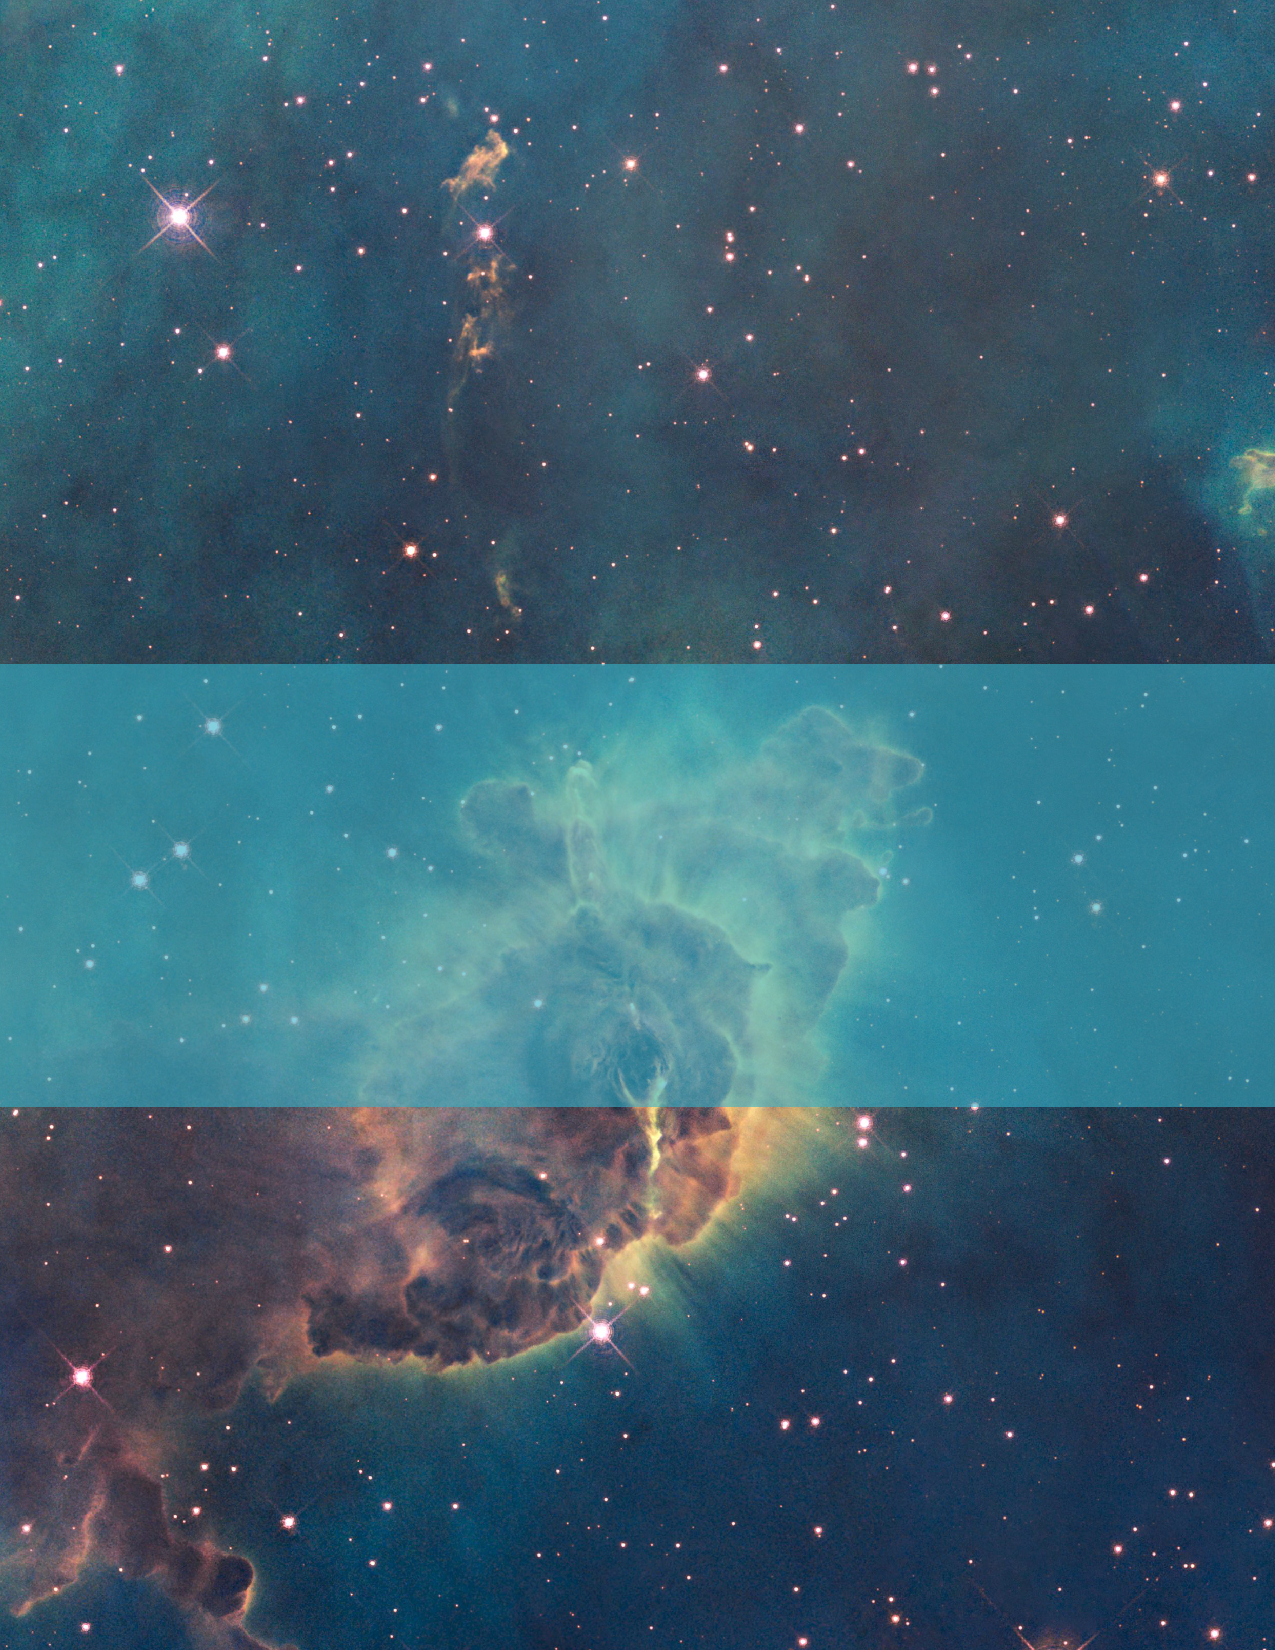
\includegraphics[scale=1.25]{esahubble}}} % Image background
\centering
\vspace*{5cm}
\par\normalfont\fontsize{35}{35}\sffamily\selectfont
\textbf{Astrophysical Fluid Dynamics}\\

\vspace*{1cm}
{\Huge Notes}\par % Author name
\endgroup

%----------------------------------------------------------------------------------------
%	COPYRIGHT PAGE
%----------------------------------------------------------------------------------------

\newpage
~\vfill
\thispagestyle{empty}

%\noindent Copyright \copyright\ 2014 Andrea Hidalgo\\ % Copyright notice

\noindent \textsc{Eliza Diggins, University of California, Berkeley}\\

\noindent \textsc{github.com/eliza-diggins}\\ % URL


%----------------------------------------------------------------------------------------
%	TABLE OF CONTENTS
%----------------------------------------------------------------------------------------

\chapterimage{head1.png} % Table of contents heading image

\pagestyle{empty} % No headers

\tableofcontents % Print the table of contents itself

%\cleardoublepage % Forces the first chapter to start on an odd page so it's on the right

\pagestyle{fancy} % Print headers again

%----------------------------------------------------------------------------------------
%	CHAPTER 1
%----------------------------------------------------------------------------------------
\chapterimage{head2.png} % Chapter heading image
\chapter{Fundamental Concepts}
As it concerns our purposes in these notes, a fluid may be (roughly) defined as
\begin{definition}[Fluid]
A fluid is some spatially distributed material which is able to freely deform. In effect, this distinguishes solids from fluids (gas and liquid). 
\end{definition}
\begin{remark}
    It isn't hard to find instances where this sort of treatment breaks down; however, in astrophysical scenarios we are almost always concerned with material which is distinctively gaseous and therefore do not care to make too much effort in refining the above definition.
\end{remark}

In classical fluid dynamics, the \textbf{incompressibility} of the flow is often introduced early and kept as a core assumption throughout. This is not a valid approximation in most astrophysical scenarios as gas is often compressed. We therefore do not benefit from any of the theory regarding incompressible flow.

\section{Elementary Definitions}
To begin our discussion, we will make some elementary remarks about important definitions and concepts.

\subsection{The Fluid Element}

\textbf{Fluid Dynamics} is, first and foremost, an \textbf{effective (ensemble) theory}, meaning it describes the collective behavior of an enormous number of discrete constituents (particles) using a small set of continuous fields, such as the mass density $\rho$ and velocity field ${\bf u}$. For this coarse-grained description to be valid, we must identify a characteristic length scale $\ell$ satisfying two key conditions:
\vspace{0.25cm}
\begin{enumerate}
    \item \textbf{Sufficiently small:} The scale $\ell$ must be much smaller than the length scales over which any relevant quantity $q$ varies appreciably. In other words, relative variations $\delta q/q$ across $\ell$ should satisfy 
\begin{equation}
    \label{eq:fluid_condition_1}
    \delta q/q \ll 1
\end{equation}
This ensures we can meaningfully associate a well-defined, approximately uniform value of $q$ to each fluid element, neglecting internal fluctuations within that element.
\end{enumerate}

In addition,

\begin{enumerate}
    \setcounter{enumi}{1}
    \item \textbf{Sufficiently statistical:} The scale $\ell$ must be large enough to contain many particles, so that microscopic, particle-level fluctuations are negligible compared to the collective, ensemble behavior. Formally, this requires the particle number density $n$ to satisfy
\begin{equation}
    \label{eq:fluid_conditions_2}
    \ell^3 n \gg 1.
\end{equation}
\end{enumerate}

\vspace{0.25cm}
The above criteria are sufficient to define a \textbf{fluid} in the context of an \textbf{effective field theory}, where the microscopic particle description is replaced by continuous fields. However, even when these conditions are met, a subtle distinction remains concerning the dynamical behavior of the system.

In general, such a fluid may retain some degree of \textbf{phase-space memory}: its present evolution can depend not only on the instantaneous values of the fluid fields, but also on the detailed history of the system's distribution function. In other words, perturbations to the microscopic particle distribution at an earlier time $\delta t$ may still influence the system's current state.

The extent to which this phase-space memory affects the dynamics depends on whether the fluid is \textbf{collisional} or \textbf{collisionless}:
\begin{itemize}
    \item In a \textbf{collisional fluid}, frequent particle interactions drive the system toward local thermodynamic equilibrium on timescales short compared to the macroscopic evolution. In this regime, the fluid fields $\rho$, ${\bf u}$, etc., contain all necessary information, and the system rapidly forgets its microscopic history. The dynamics are thus determined entirely by local field values and their gradients. In order for a fluid to be \textbf{collisional}, we require that the \textbf{mean free path} between interactions satisfy
\begin{equation}
    \label{eq:fluid_condition_collisional}
    \lambda_{\rm mfp} \ll \ell.
\end{equation}
Recalling that
\begin{equation}
    \lambda_{\rm mfp} = \frac{1}{n\sigma} \implies n\sigma \gg \ell^{-1}.
\end{equation}
    
    \item In a \textbf{collisionless fluid}, particle interactions are sufficiently rare or absent that the system does not locally equilibrate. Instead, the evolution retains dependence on the detailed particle distribution function in phase space. In this case, a purely field-based description is incomplete, and additional information about the microscopic state—often encapsulated by the distribution function $f({\bf x}, {\bf p}, t)$—is required.
\end{itemize}

Thus, while the field-theoretic description of fluids is powerful, its completeness depends critically on whether the underlying system rapidly equilibrates (collisional) or preserves phase-space structure over dynamical timescales (collisionless).

\subsection{View of Fluid Dynamics: Eulerian and Lagrangian Perspectives}

Fluid dynamics can be formulated from two mathematically distinct but physically equivalent viewpoints: the \textbf{Eulerian} and the \textbf{Lagrangian} descriptions. These perspectives differ in how they \textbf{label fluid elements} and in what domain the physical fields are defined.

\vspace{0.2cm}
\begin{center}
\textit{
Consider a continuum which, at initial time \( t = 0 \), occupies a reference configuration \( \mathcal{C}_0 \subset \mathbb{R}^3 \). As time progresses, the fluid deforms into new spatial configurations \( \mathcal{C}_t \), flowing and evolving through space. This notion leads us to the rather formal definition of the \textbf{flow map}, which tells us how to go from one deformation space to a later one.
}
\end{center}
\vspace{0.2cm}
\begin{definition}[Flow Map / Configuration Map]
Let \( \mathcal{C}_0 \subset \mathbb{R}^3 \) be the reference configuration describing the fluid position at $t=t_0$. The \textbf{flow map}
\[
\boldsymbol{\varphi}: \mathcal{C}_0 \times \mathbb{R} \to \mathbb{R}^3
\]
is defined by
\[
\boldsymbol{\varphi}(\mathbf{X}, t) = \mathbf{x},
\]
where \( \mathbf{X} \in \mathcal{C}_0 \) is the \textbf{label} of a material particle (its initial position), and \( \boldsymbol{\varphi}(\mathbf{X}, t) \) gives its position in physical space at time \( t \). For each fixed \( t \), the map \( \boldsymbol{\varphi}_t := \boldsymbol{\varphi}(\cdot, t) \) takes the reference configuration to the \textbf{current configuration} \( \mathcal{C}_t = \boldsymbol{\varphi}_t(\mathcal{C}_0) \subset \mathbb{R}^3 \).
\end{definition}
\vspace{0.2cm}

This flow map naturally defines the velocity field:
\[
\mathbf{u}(\mathbf{x}, t) = \left. \frac{\partial \boldsymbol{\varphi}}{\partial t}(\mathbf{X}, t) \right|_{\mathbf{X} = \boldsymbol{\varphi}^{-1}(\mathbf{x}, t)}.
\]

The unfortunate outcome of this picture is that there are \textbf{two equally good ways to look at the world}. We could label every particle based on $\mathcal{C}_0$ and then use $\varphi$ to move forward into $C_t$, or we could label particles based on $C_t$ and go backward with $\varphi^{-1}$. These are both perfectly good ways to look at the world and they are beneficial in different scenarios. Formally,
\vspace{0.5cm}
\begin{definition}[Eulerian Field]
\label{def:Eulerian}
In the \textbf{Eulerian} description, fluid properties are described as functions on the \textbf{current configuration} \( \mathcal{C}_t \subset \mathbb{R}^3 \). That is, a scalar field \( \psi \) (such as pressure, density, etc.) is defined by:
\[
\psi: \mathcal{C}_t \to \mathbb{R}, \quad \mathbf{x} \mapsto \psi(\mathbf{x}, t),
\]
where \( \mathbf{x} \in \mathcal{C}_t \) is a point in space occupied by the fluid at time \( t \), and \( \psi(\mathbf{x}, t) \) gives the value of the field at that location.

If we wish to express this quantity in terms of the \textbf{reference configuration} \( \mathcal{C}_0 \), we must \textbf{pull back} the field along the flow map \( \boldsymbol{\varphi}: \mathcal{C}_0 \times \mathbb{R} \to \mathcal{C}_t \). The associated Lagrangian field is:
\[
\Psi(\mathbf{X}, t) := \psi(\boldsymbol{\varphi}(\mathbf{X}, t), t),
\]
where \( \mathbf{X} \in \mathcal{C}_0 \) labels a material particle.

Conversely, the Eulerian field is the \textbf{pushforward} of the \textbf{Lagrangian field}:
\[
\psi(\mathbf{x}, t) = \Psi(\boldsymbol{\varphi}^{-1}(\mathbf{x}, t), t), \quad \text{for } \mathbf{x} \in \mathcal{C}_t.
\]
\end{definition}
\vspace{0.1cm}
As was hinted about in definition~\ref{def:Eulerian}, the \textbf{Lagrangian view} is effectively the inverse:
\vspace{0.1cm}
\begin{definition}[Lagrangian Field]
\label{def:Lagrangian}
In the \textbf{Lagrangian} description, fluid properties are described as functions on the \textbf{reference configuration} \( \mathcal{C}_0 \subset \mathbb{R}^3 \), which labels material particles by their initial positions. 

Let \( \boldsymbol{\varphi}: \mathcal{C}_0 \times \mathbb{R} \to \mathbb{R}^3 \) be the \textbf{flow map}, such that for each material label \( \mathbf{X} \in \mathcal{C}_0 \), \( \boldsymbol{\varphi}(\mathbf{X}, t) \) gives the spatial position of that particle at time \( t \).

Then, for a physical observable \( \psi: \mathcal{C}_t \to \mathbb{R} \), the corresponding \textbf{Lagrangian field} is defined by the \textbf{pullback} of \( \psi \) along \( \boldsymbol{\varphi} \):
\[
\Psi: \mathcal{C}_0 \times \mathbb{R} \to \mathbb{R}, \qquad \Psi(\mathbf{X}, t) := \psi(\boldsymbol{\varphi}(\mathbf{X}, t), t).
\]

That is, \( \Psi(\mathbf{X}, t) \) gives the value of the field as experienced by the material particle labeled by \( \mathbf{X} \), as it evolves in time.

Conversely, the Eulerian field can be recovered by the \textbf{pushforward}:
\[
\psi(\mathbf{x}, t) = \Psi(\boldsymbol{\varphi}^{-1}(\mathbf{x}, t), t), \quad \text{for } \mathbf{x} \in \mathcal{C}_t.
\]
\end{definition}
\vspace{0.5cm}

\begin{remark}
    In general, \textbf{Eulerian} methods are more powerful for most uses analytically. We are generally more interested in the benefits of having a simple, stationary coordinate system than the benefits of being able to track individual packets of material. There are some exceptions to this however. 

    In computational fluid dynamics, this is dramatically different as both approaches lead to powerful computational methods.
\end{remark}
\vspace{0.5cm}

We can naturally connect the \textbf{Eulerian} and \textbf{Lagrangian} descriptions of fluid dynamics. Consider a flow characterized by a \textbf{velocity field} ${\bf u}({\bf r}, t)$ and a scalar field $\psi({\bf r}, t)$ defined in the Eulerian frame.

Suppose a fluid particle is initially located at position ${\bf r}_0$ at time $t = 0$. After an infinitesimal time interval $\delta t$, the particle moves to
\[
{\bf r}_1 = {\bf r}_0 + {\bf u}({\bf r}_0, 0) \, \delta t.
\]
The change in $\psi$ experienced by the particle along its trajectory—the \textbf{Lagrangian change}—is given by
\[
\delta \psi_{\rm lagrangian} = \psi({\bf r}_1, \delta t) - \psi({\bf r}_0, 0).
\]

Assuming $\psi$ is sufficiently smooth (at least $C^2$ continuous), we expand $\psi$ to first order:
\[
\psi({\bf r}_1, \delta t) \approx \psi({\bf r}_0, 0) + \delta {\bf r} \cdot \nabla \psi + \delta t \, \frac{\partial \psi}{\partial t} + \mathcal{O}(\delta {\bf r}^2, \delta t^2).
\]
Since $\delta {\bf r} = {\bf u} \, \delta t$, this becomes:
\[
\delta \psi_{\rm lagrangian} = {\bf u} \cdot \nabla \psi \, \delta t + \frac{\partial \psi}{\partial t} \, \delta t + \mathcal{O}(\delta t^2).
\]
Dividing both sides by $\delta t$ and taking the limit $\delta t \to 0$, we obtain the \textbf{material derivative} (or \textbf{Lagrangian derivative}):
\begin{equation}
    \label{eq:euler-lagrange-convert}
    \boxed{
    \frac{d \psi_{\rm lagrangian}}{dt} = \frac{D \psi}{D t} = \frac{\partial \psi}{\partial t} + {\bf u} \cdot \nabla \psi.}
\end{equation}

This expression shows how the time rate of change of a field $\psi$ as experienced by a moving fluid element (Lagrangian perspective) relates to the local, fixed-position time derivative and spatial variations in the Eulerian description.
\begin{remark}
    It is important to remember that the \textbf{Lagrangian derivative} is NOT written in the lagrangian frame. Really, we are representing $D/Dt$ in the Eulerian frame as $\partial_t + {\bf u} \cdot \nabla$,  which then reminds us that, formally, we regard ${\bf u}$ as ${\bf u}({\bf x},t) = {\bf u}(\varphi({\bf X},t),t)$ and $\nabla$ as $\nabla_{\bf x}$, not $\nabla_{\bf X}$.
\end{remark}

\section{Structure of the Velocity Field}

An extremely important field present in fluid dynamical flows is the \textbf{velocity field} ${\bf u}$, which describes the instantaneous velocity at a point $(x,t) \in \mathbb{R}^d \times \mathbb{R}$. There are a number of things to be said about this velocity field which are relevant throughout this subject.

\subsection{The Velocity Gradient}

A common construct in fluid kinematics is the \textbf{velocity gradient}, which is a $(1,1)$ tensor field over the domain defined such that
\[
{\bf V}(\omega, X) = \omega\!\left(X({\bf u})\right).
\]
In a particular basis, this is equivalent to
\[
V_\mu^\nu = \nabla_\mu u^\nu,
\]
where $\nabla_\mu$ is the \textbf{covariant derivative}. \rmk{In Cartesian coordinates, this may be taken as the standard gradient.}

\par
Like any rank-2 tensor, the velocity gradient can be decomposed into its symmetric and antisymmetric parts:
\[
V_{\mu}^\nu 
= \tfrac{1}{2}\left(\nabla_\mu u^\nu + \nabla_\nu u^\mu\right) 
+ \tfrac{1}{2}\left(\nabla_\mu u^\nu - \nabla_\nu u^\mu\right) 
= S_{\mu}^\nu + \Omega_\mu^\nu.
\]

\subsubsection*{The Rate of Strain Tensor}

The symmetric component is called the \textbf{rate-of-strain tensor}:
\vspace{0.5cm}
\begin{definition}[Rate-of-Strain Tensor]
The \textbf{rate-of-strain tensor} (or \textbf{strain rate tensor}) is defined by
\[
S_{\mu}^\nu = \tfrac{1}{2}\left(\nabla_\mu u^\nu + \nabla_\nu u^\mu\right).
\]
It encodes both the isotropic \emph{expansion} of fluid elements and the \emph{shear} which distorts their shape without changing volume.
\end{definition}
\vspace{0.5cm}

The trace of $S_{\mu\nu}$ yields the \textbf{expansion scalar}:
\[
\theta = \nabla_\mu u^\mu,
\]
which measures the local volumetric dilation of the flow. Subtracting this isotropic part leaves the \textbf{shear tensor}:
\[
\sigma_{\mu\nu} = S_{\mu\nu} - \tfrac{1}{3}\theta\, g_{\mu\nu},
\]
a symmetric, trace-free object describing pure shape distortion. 

\par
This decomposition is directly relevant for fluid dynamics: in Newtonian fluids the viscous stress tensor is proportional to $S_{\mu\nu}$, with separate coefficients (bulk and shear viscosity) multiplying its trace and trace-free parts. Thus $S_{\mu\nu}$ is the quantity that determines how velocity gradients are converted into internal stresses and, ultimately, into heat through viscous dissipation.

\subsubsection*{The Vorticity Tensor}

The antisymmetric component is called the \textbf{vorticity tensor}:
\vspace{0.5cm}
\begin{definition}[Vorticity Tensor]
\label{def:vorticity}
The \textbf{vorticity tensor} is defined by
\[
\Omega_{\mu}{}^{\nu} = \tfrac{1}{2}\left(\nabla_\mu u^\nu - \nabla_\nu u^\mu\right).
\]
It encodes the local \emph{rotation} of fluid elements, i.e.\ the rigid-body spin of a small fluid parcel.
\end{definition}
\vspace{0.5cm}

In three-dimensional Euclidean space, $\Omega_{\mu\nu}$ corresponds directly to the familiar \textbf{vorticity vector} 
\[
\boldsymbol{\omega} = \nabla \times \mathbf{u},
\]
which provides an intuitive picture of the local axis of rotation of the flow. 

\par
Vorticity is central in the classification of flows. When $\Omega_{\mu\nu} = 0$, the flow is called \textbf{irrotational}, and the velocity can be expressed as the gradient of a scalar potential. This condition underlies many classical results such as Bernoulli’s theorem. Conversely, nonzero vorticity characterizes rotational flows, vortex dynamics, and ultimately turbulence, where the stretching and diffusion of vorticity dominate the behavior of the system.

\subsubsection*{Summary}

Altogether, the velocity gradient admits a canonical decomposition:
\[
\nabla_\mu u_\nu = \sigma_{\mu\nu} + \tfrac{1}{3}\theta\, g_{\mu\nu} + \Omega_{\mu\nu},
\]
into \emph{shear}, \emph{expansion}, and \emph{vorticity}. Each piece has distinct physical significance:
\begin{itemize}
  \item $\theta$ controls local compression or expansion of the fluid.
  \item $\sigma_{\mu\nu}$ governs shape distortion and is directly linked to viscous stresses and dissipation.
  \item $\Omega_{\mu\nu}$ (or $\boldsymbol{\omega}$) measures local rigid-body rotation, with vanishing vorticity defining irrotational flow.
\end{itemize}
This decomposition provides a complete kinematic description of how fluid elements evolve in time.

\begin{bigidea}
The \textbf{velocity gradient} $\nabla_\mu u_\nu$ can always be decomposed into three geometrically and physically distinct parts:
\[
\nabla_\mu u_\nu = \sigma_{\mu\nu} + \tfrac{1}{3}\theta\, g_{\mu\nu} + \Omega_{\mu\nu}.
\]
This canonical splitting encodes the full local behavior of a fluid element:
\begin{itemize}
  \item $\theta$: the \textbf{expansion scalar}, measuring isotropic compression or dilation (volume change).
  \item $\sigma_{\mu\nu}$: the \textbf{shear tensor}, capturing pure shape distortion. It is the driver of viscous stresses and dissipation.
  \item $\Omega_{\mu\nu}$: the \textbf{vorticity tensor}, representing rigid-body rotation of the fluid element. In 3D, this is equivalent to the familiar vorticity vector $\boldsymbol{\omega} = \nabla \times \mathbf{u}$, whose vanishing defines \emph{irrotational flow}.
\end{itemize}
Together, these components form the cornerstone of fluid kinematics: they describe how small parcels of fluid move, deform, and spin, and they connect directly to the physics of viscosity, potential flows, and turbulence.
\end{bigidea}

\chapter{The Fluid Equations}
In this section, we will derive the critical equations of fluid dynamics: the so-called \textbf{Euler Equations}. In effect, these are derived from 3 core principles:

\begin{enumerate}
    \item \textbf{Conservation of Mass}: leads to the \emph{conservation equation}.
    \item \textbf{Conservation of Energy / Momentum}: lead to the Euler equations.
\end{enumerate}

\section{The Continuity Equation}

Consider a fluid with a conserved density field $\psi$ (generally the \textbf{mass density}). In some region $V$, the total amount of the conserved field is
\[
\Psi = \int_V \psi dV.
\]
Now, this may flow in / out of the volume or be created / destroyed within the volume. In some time $\delta t$, we describe the created / destroyed quantity as
\[
\Delta \Psi_{\rm internal} = \int_V \delta \psi dV
\]
Additionally, there is some flow in / out of the surface
\[
\Delta \Psi_{\rm flux} = dt\oint_{\partial V} \psi {\bf u} \cdot d{\bf S}.
\]
If \textbf{no material is created / destroyed}, then
\[
\frac{d\Psi}{dt} = -\oint_{\partial V} \psi \;{\bf u} \cdot d{\bf S} 
\]
By \textbf{divergence theorem},
\[
-\oint_{\partial V} {\bf X} \cdot d{\bf S} = -\int_V \nabla \cdot {\bf X} dV \implies \oint_{\partial V} \psi {\bf u} \cdot d{\bf S} = \int_V \nabla \cdot (\psi {\bf u}) dV.
\]
Therefore,
\[
\frac{d\Psi}{dt} = \int_V \frac{\partial\psi}{\partial t} dV = - \int_V \nabla \cdot (\psi {\bf u}) dV.
\]
In the limit as $V \to 0$, this becomes
\begin{equation}
\label{eq:conservation-equation-eulerian}
\boxed{
\frac{\partial\psi}{\partial t} + \nabla \cdot (\psi {\bf u}) = 0.\;\text{Eulerian.}
}
\end{equation}
\begin{remark}
    In most cases, we are chiefly concerned with the density $\rho$, in which case we have
    \[
    \frac{\partial\rho}{\partial t} + \nabla \cdot (\rho {\bf u}) = 0
    \]
    In the frequent case (in classical fluid dynamics) where $\rho$ is a constant of the flow, you can pull it out; however, this is not generally the case in compressible gas flows.
\end{remark}

To write the above result in \textbf{Lagrangian form}, we need only remember that (equation~\ref{eq:euler-lagrange-convert})
\[
\frac{\partial \psi_{\rm Eulerian}}{\partial t} = \frac{D\psi}{Dt} - {\bf u} \cdot \nabla \psi.
\]
\rmk{Recall that $\nabla \cdot (\rho {\bf u}) = \partial_k (\rho u^k) = \rho \partial_ku^k + u^k \partial_k \rho = \rho \nabla \cdot {\bf u} + {\bf u} \cdot \nabla \rho.$} Thus, substituting into equation~\ref{eq:conservation-equation-eulerian}, we find
\begin{equation}
   \label{eq:conservation-equation-lagrangian}
   \boxed{
    \frac{D\rho}{Dt} + \rho \nabla \cdot {\bf u} = 0.\;\text{Lagrangian.}}
\end{equation}
\begin{remark}
    The intuition here is not as easy to see on inspection. Imagine yourself floating along in the flow. The first term $D\rho/Dt$ describes how the \textbf{comoving density} behaves (the density you feel). Now, what should that intuitively be tied to? Well clearly to the density of the particles around you. They are all also moving with the flow, so as long as the flow lines remain totally parallel we don't get any change in density. If the flow lines converge, then the density will clearly go up as particles get pressed closer. The natural measure of that "convergence" is the \textbf{divergence of the velocity field}.

    Notice that both forms of the equation have their "problem terms." The Eulerian approach requires $\nabla \cdot (\psi{\bf u})$, which may be tricky to evaluate. Meanwhile, the Lagrangian term only requires $\nabla \cdot {\bf u}$ but also requires $D\rho/Dt$.
\end{remark}
\begin{remark}
    Consider the scenario where $D\rho/Dt = 0.$ We see immediately that this requires $\nabla \cdot {\bf u} = 0$, so the fluid is \textbf{solenoidal} (divergenceless). This is a characteristic aspect of \textbf{divergence free flows} or \textbf{incompressible flows}, which occur in many limits.
\end{remark}
\section{Vector Conservation Laws}

Just as we did for the scalar field $\psi$, we might also be interested in the conservation of a vector density field ${\bf \Psi}$ defined on the domain. This is a \textbf{trickier calculation}; however, it has a massive role in the nature of fluid dynamics, especially in the conservation of momentum.

\begin{remark}
    For a \textbf{vector density}, each component of the field must be conserved as in the scalar case; however, flux in / out of the surface in a particular index $i$ may couple with the $j$ component in the adjacent region. This was a consideration which was not necessary in the treatment of the scalar case.
\end{remark}

Consider a region $V$ of the domain with total quantity of $\psi_k$:
\[
\Psi_k = \int_V \psi_k \; dV.
\]
As in the scalar case, changes to $\Psi_k$ may arise from creation/annihilation within $V$ and flux across the boundary $\partial V$. The creation/annihilation is straightforward:
\[
\Delta \Psi_{k,\;{\rm internal}} = \int_V \frac{\partial \psi_k}{\partial t} \; dV.
\]
However, the movement across the membrane is \textbf{not as simple to describe}, since the vector field may not transport identically across all orientations of the membrane, nor in all components. We therefore introduce the \textbf{Flux Tensor} $\Sigma^k_j$, defined such that:
\[
\Delta \Psi_{k,\;{\rm flux}} = \oint_{\partial V} \Sigma^k_j \; dS^j.
\]
\rmk{Note that we have made a sign convention here which needs to be kept track of...}
Here, $dS^j$ is the oriented surface area element in the $j^{\rm th}$ direction, and $\Sigma^k_j$ expresses the flux of the $k^{\rm th}$ component of the conserved vector through surfaces with orientation in the $j^{\rm th}$ direction. The change in the total $\Psi$ in a time $\Delta t$ is thus
\[
\Delta \Psi = \int_V \frac{\partial \psi_k}{\partial t} \; dV + \oint \Sigma_j^k \;dS^j = \int_V \frac{\partial \psi_k}{\partial t} + \partial_j\Sigma_j^k\; dV \Delta t
\]
Now, the LHS provides source terms to the equation and we therefore have that, for some set of sources ${\bf f}$,
\[
\frac{\partial \boldsymbol{\psi}}{\partial t} + \nabla \cdot \boldsymbol{\Sigma} = {\bf f}.
\]
Since $V$ is arbitrary, the integrands must be equal everywhere, leading to the \textbf{general vector conservation law}:
\begin{equation}
\boxed{
\frac{\partial \psi_k}{\partial t} + \partial_j \Sigma^k_j = 0.
}
\end{equation}
In \textbf{vector notation}, this is
\[
\frac{\partial{\bf \Psi}}{\partial t} + \nabla \cdot {\bf \Sigma} = 0,\;\text{Eulerian.}
\]

\subsection{Momentum Conservation}

With the general form of a \textbf{vector conservation law} in hand, we now want to derive the explicit form of the flux tensor $\Sigma$ for the case of momentum conservation. The relevant vector density field is the \textbf{momentum density}:
\[
{\bf p} = \rho {\bf u},
\]
where $\rho$ is the mass density and ${\bf u}$ is the velocity field.

There are \textbf{two distinct physical mechanisms} by which momentum is transported in a fluid:

\begin{enumerate}
    \item \textbf{Advection}: Material crosses the boundary $\partial V$ carrying its momentum with it. The mass flux across a surface with oriented area element $dS^j$ is $\rho u_j \, dS^j$. Since each unit of mass carries momentum ${\bf p}$, the $k^{\rm th}$ component of momentum advected across the surface is:
    \[
    \Delta p^k_{\rm advective} = \rho u^k u_j \, dS^j.
    \]

    \item \textbf{Internal Stresses}: Even without bulk motion, microscopic interactions between particles on either side of the boundary may transfer momentum. These are summarized by the \textbf{stress tensor} $\sigma^k_j$, defined such that the $k^{\rm th}$ component of momentum transferred per unit area per unit time across a surface with normal $\hat{n}^j$ is:
    \[
    \Delta p^k_{\rm stress} = \sigma^k_j \, \hat{n}^j.
    \]
\end{enumerate}

Combining these mechanisms, the total momentum flux tensor takes the form:
\[
\Sigma^k_j = \rho u^k u_j + \sigma^k_j.
\]

The general vector conservation law for momentum density reads:
\[
\frac{\partial p_k}{\partial t} + \partial_j \Sigma^k_j = 0,
\]
or explicitly:
\[
\frac{\partial (\rho u_k)}{\partial t} + \partial_j \left( \rho u_k u^j + \sigma^k_j \right) = 0.
\]

In vector notation, this becomes:
\[
\frac{\partial {\bf p}}{\partial t} + \nabla \cdot ({\bf p} \otimes {\bf u}) + \nabla \cdot \boldsymbol{\sigma} = 0,
\]
where:
\begin{itemize}
    \item ${\bf p} \otimes {\bf u}$ denotes the outer product (dyadic product) of momentum and velocity, producing a rank-2 tensor with components $p^k u_j = \rho u^k u_j$,
    \item $\boldsymbol{\sigma}$ is the stress tensor.
\end{itemize}

This formulation clearly separates:
\begin{itemize}
    \item Momentum transport due to advection (${\bf p} \otimes {\bf u}$),
    \item Momentum exchange due to internal stresses ($\boldsymbol{\sigma}$).
\end{itemize}

In \textbf{some cases}, we may have \textbf{external sources of momentum}, leading us to
\[
\frac{\partial {\bf p}}{\partial t} + \nabla \cdot ({\bf p} \otimes {\bf u}) + \nabla \cdot \boldsymbol{\sigma} = {\bf F}_{\rm ext}.
\]
\begin{remark}
    We also might characterize the entire RHS as a stress tensor:
    \[
    \boldsymbol{\sigma} = \left({\bf p} \otimes {\bf u} + P{\bf I}\right),
    \]
    in which case, we have
    \[
    \frac{\partial {\bf p}}{\partial t} + \nabla \cdot \boldsymbol{\sigma} ={\bf F}_{\rm ext}.
    \]
\end{remark}
\textbf{much more can be done with a bit more work.}

\subsection{The Stress Tensor}

We have, so far, derived the critical equation
\[
\boxed{
\frac{\partial {\bf p}}{\partial t} + \nabla \cdot ({\bf p} \otimes {\bf u}) + \nabla \cdot \boldsymbol{\sigma} = {\bf F}_{\rm ext}.}
\]
for a very general $\boldsymbol{\sigma}$, these equations can be quite difficult to solve; however, we can make quite a bit of progress on physical arguments about the stress tensor. In this section, we'll take some time to explore these behaviors before proceeding.
\vspace{0.25cm}
\begin{theorem}[The stress tensor is symmetric]
\label{thrm:stress-is-symmetric}
Let ${\bf p}$ be the momentum of a particular fluid flow with velocity field ${\bf u}$ and density field $\rho$. Regardless of the nature of the system, the \textbf{stress tensor} $\sigma_{ij}$ is everywhere symmetric.
\end{theorem}
\rmk{In fact, by the same logic, you can show that ANY \textbf{flux tensor} in a momentum conservation law MUST have these properties for the same reason. This makes the flux tensor for momentum special in that it must ALWAYS be symmetric.}
\begin{proof}
The intuition behind this is relatively simple. Consider a small control volume of fluid with negligible size. If the off-diagonal elements of the stress tensor are not symmetric, the internal forces will generate a net torque proportional to the surface area of the control volume. As the size of the volume shrinks to zero, the torque remains finite, implying the possibility of unbounded angular acceleration — contradicting the assumption of local mechanical equilibrium.

We now present the formal derivation based on the conservation of angular momentum.

The total angular momentum of a region $V$ is given by:
\[
L^k = \int_V \epsilon^{kij} x_i \rho u_j \; dV,
\]
where:
\begin{itemize}
    \item $\epsilon^{kij}$ is the Levi-Civita symbol,
    \item $x_i$ is the position vector,
    \item $\rho u_j$ is the $j^{\rm th}$ component of the momentum density.
\end{itemize}

The rate of change of angular momentum is:
\[
\frac{d L^k}{dt} = \int_V \epsilon^{kij} x_i \frac{\partial (\rho u_j)}{\partial t} \; dV.
\]

Applying the momentum conservation equation:
\[
\frac{\partial (\rho u_j)}{\partial t} + \partial_m \Sigma^m_j = 0,
\]
we substitute:
\[
\frac{d L^k}{dt} = - \int_V \epsilon^{kij} x_i \partial_m \Sigma^m_j \; dV.
\]

Using the product rule and the divergence theorem:
\[
\frac{d L^k}{dt} = - \oint_{\partial V} \epsilon^{kij} x_i \Sigma^m_j \; dS_m + \int_V \epsilon^{kij} \Sigma^m_j \delta_{im} \; dV.
\]

The first term represents the torque exerted on the boundary of the region, which may be nonzero due to external forces. The second term simplifies using $\delta_{im}$:
\[
\frac{d L^k}{dt} = - \oint_{\partial V} \epsilon^{kij} x_i \Sigma^m_j \; dS_m + \int_V \epsilon^{kij} \Sigma^i_j \; dV.
\]

In the absence of internal microscopic torques (body couples), conservation of angular momentum requires that the internal torque contribution vanishes identically:
\[
\int_V \epsilon^{kij} \Sigma^i_j \; dV = 0.
\]

Since $V$ is arbitrary, the integrand itself must vanish pointwise:
\[
\epsilon^{kij} \Sigma^i_j = 0.
\]

The Levi-Civita symbol is antisymmetric in $i$ and $j$, implying that the antisymmetric part of $\Sigma^i_j$ must vanish. Explicitly, we can decompose:
\[
\Sigma^i_j = \Sigma^{(ij)} + \Sigma^{[ij]},
\]
where:
\[
\Sigma^{(ij)} = \frac{1}{2} \left( \Sigma^i_j + \Sigma^j_i \right), \quad \Sigma^{[ij]} = \frac{1}{2} \left( \Sigma^i_j - \Sigma^j_i \right).
\]

The expression $\epsilon^{kij} \Sigma^i_j = 0$ requires the antisymmetric part $\Sigma^{[ij]}$ to vanish identically. Therefore, the stress tensor is symmetric:
\[
\boxed{ \Sigma^i_j = \Sigma^j_i }.
\]

In particular, for the internal stress tensor $\sigma^i_j$, this symmetry property holds:
\[
\sigma^i_j = \sigma^j_i.
\]

Thus, the stress tensor is symmetric everywhere, consistent with conservation of angular momentum in the absence of internal body torques.

\end{proof}
\vspace{0.5cm}
Theorem~\ref{thrm:stress-is-symmetric} gives us a few very interesting corollaries:

\begin{corollary}
    For any stress tensor $\sigma_{ij}$, there is a coordinate frame (orthogonal transformation) in which $\sigma$ is \textbf{diagonalized}. In this frame, there are no shear forces and the expansion / contraction of fluid elements is more directly understood.
\end{corollary}

\begin{corollary}
    Any stress tensor may be \textbf{decomposed} into its \textbf{isotropic} and \textbf{deviatoric} components:
    
    \begin{itemize}
        \item The \textbf{isotropic component} is of the form $-p \delta_{ij}$, where $p$ is the \textbf{very familiar quantity of pressure}.
        \item The \textbf{deviatoric component} is effectively everything else: $\tau_{ij}$. It describes the shears and viscous effects.
    \end{itemize}
\end{corollary}

\section{Euler's Equations}

We are now in a position to derive the \textbf{Euler equations} — the fundamental equations governing the motion of an \emph{inviscid} (non-viscous) fluid. These equations follow naturally by simplifying the general momentum conservation law under the assumption that viscous stresses vanish and only isotropic pressure remains.

\vspace{0.25cm}
\subsubsection*{Momentum Conservation in General Form}

Recall the momentum conservation equation:
\[
\frac{\partial {\bf p}}{\partial t} + \nabla \cdot ({\bf p} \otimes {\bf u}) + \nabla \cdot \boldsymbol{\sigma} = {\bf F}_{\rm ext},
\]
where:
\begin{itemize}
    \item ${\bf p} = \rho {\bf u}$ is the momentum density,
    \item $\boldsymbol{\sigma}$ is the internal stress tensor,
    \item ${\bf F}_{\rm ext}$ represents external body forces (e.g., gravity).
\end{itemize}

For an inviscid fluid, there are no shear or viscous stresses. The only internal stress is the isotropic pressure, so:
\[
\sigma_{ij} = -p \delta_{ij},
\]
where:
\begin{itemize}
    \item $p$ is the pressure,
    \item $\delta_{ij}$ is the Kronecker delta.
\end{itemize}

Substituting into the momentum conservation equation:
\[
\frac{\partial (\rho u_k)}{\partial t} + \partial_j \left( \rho u_k u^j \right) + \partial_j \left( -p \delta^k_j \right) = F^k_{\rm ext}.
\]

Simplifying:
\[
\frac{\partial (\rho u_k)}{\partial t} + \partial_j \left( \rho u_k u^j \right) = - \partial_k p + F^k_{\rm ext}.
\]

\subsection*{Expanding with the Continuity Equation}

We can rewrite the time derivative term using the product rule:
\[
\frac{\partial (\rho u_k)}{\partial t} = \rho \frac{\partial u_k}{\partial t} + u_k \frac{\partial \rho}{\partial t},
\]
and similarly expand the divergence term:
\[
\partial_j \left( \rho u_k u^j \right) = \rho u^j \partial_j u_k + u_k \partial_j ( \rho u^j ).
\]

Thus, the momentum equation becomes:
\[
\rho \frac{\partial u_k}{\partial t} + u_k \frac{\partial \rho}{\partial t} + \rho u^j \partial_j u_k + u_k \partial_j ( \rho u^j ) = - \partial_k p + F^k_{\rm ext}.
\]

We now use the continuity equation (conservation of mass):
\[
\frac{\partial \rho}{\partial t} + \nabla \cdot ( \rho {\bf u} ) = 0,
\]
or explicitly:
\[
\frac{\partial \rho}{\partial t} + \partial_j ( \rho u^j ) = 0.
\]

Substituting this into the momentum equation, notice:
\[
u_k \left( \frac{\partial \rho}{\partial t} + \partial_j ( \rho u^j ) \right) = 0.
\]

Therefore, the momentum equation simplifies to:
\[
\rho \left( \frac{\partial u_k}{\partial t} + u^j \partial_j u_k \right) = - \partial_k p + F^k_{\rm ext}.
\]

\subsection*{Lagrangian Form of the Euler Equations}

The left-hand side of the above is the \textbf{material derivative} of $u_k$:
\[
\frac{D u_k}{D t} = \frac{\partial u_k}{\partial t} + u^j \partial_j u_k.
\]

Thus, the \textbf{Lagrangian form} of the Euler equations is:
\begin{equation}
\label{eq:momentum_lagrangian}
\boxed{
\rho \frac{D {\bf u}}{D t} = - \nabla p + {\bf F}_{\rm ext}.
}
\end{equation}

Intuitively, this is the co-moving conservation of momentum equation, which makes a lot of sense on examination of its various terms and in analogy with the familiar form of Newton's 2nd law.

\subsection*{Eulerian Form of the Euler Equations}

Alternatively, from the stationary (Eulerian) perspective, we can simply transform the equation as
\[
\rho \partial_t {\bf u} + \rho {\bf u}\cdot \nabla {\bf u} = - \nabla p + {\bf F}_{\rm ext}.
\]

This is equivalent to 
\[
\frac{\partial {\bf p}}{\partial t} + \nabla \cdot ({\bf p} \otimes {\bf u}) + \nabla \cdot \boldsymbol{\sigma} = {\bf F}_{\rm ext},
\]
after reduction of the stress tensor and inclusion of the conservation of mass.

\begin{remark}
    In the Lagrangian viewpoint, you imagine yourself drifting along with a fluid parcel. You directly experience how the velocity of the parcel changes over time as a result of local pressure gradients and external forces, such as gravity. The material derivative $D{\bf u}/Dt$ captures this physical acceleration of the parcel.
\end{remark}

\subsection*{Summary of the Inviscid Euler Equations}

For an inviscid, compressible fluid with mass density $\rho$, velocity field ${\bf u}$, and pressure $p$, the governing equations are:

\begin{enumerate}
    \item \textbf{Conservation of Mass (Continuity Equation)}:
    \[
    \frac{\partial \rho}{\partial t} + \nabla \cdot ( \rho {\bf u} ) = 0.
    \]

    \item \textbf{Conservation of Momentum (Euler Equations)}:
    \[
    \rho \frac{D {\bf u}}{D t} = - \nabla p + {\bf F}_{\rm ext}.
    \]
\end{enumerate}

These two equations form the foundation of inviscid fluid dynamics. They are generally closed by an \textbf{equation of state} relating pressure $p$ to $\rho$ and potentially other thermodynamic quantities, especially in compressible flows.

\section{Viscosity}
In many astrophysical settings, viscosity can often be neglected. However, when it does become relevant, it plays a crucial role in the dynamics. Intuitively, \textbf{viscous forces} arise from interactions between neighboring fluid elements that are moving at different velocities. These internal forces act to \textbf{resist deformation} and \textbf{dissipate energy} within the fluid.

\vspace{0.25cm}

\subsection{Velocity Gradients and Deformation}
Before discussing viscosity itself, we first need to introduce some ideas about the velocity field. The basic input to viscosity is the \textbf{velocity gradient tensor}:
\[
\nabla_\ell u_k = \frac{\partial u_k}{\partial x_\ell},
\]
which quantifies how the velocity varies in space and therefore how a fluid element is being deformed or rotated. 

As with all rank-2 tensors, the velocity gradient can be uniquely decomposed into symmetric and antisymmetric parts:
\[
\nabla_\ell u_k = 
\underbrace{\tfrac{1}{2}\left(\nabla_\ell u_k + \nabla_k u_\ell\right)}_{\text{Symmetric part}} \;+\;
\underbrace{\tfrac{1}{2}\left(\nabla_\ell u_k - \nabla_k u_\ell\right)}_{\text{Antisymmetric part}}.
\]

Both of these components play important roles in fluid dynamics and have special names.

\begin{definition}[Rate-of-Strain Tensor]
The \textbf{rate-of-strain tensor} is the symmetric part of the velocity gradient:
\[
S_{k\ell} = \tfrac{1}{2}\left(\nabla_\ell u_k + \nabla_k u_\ell\right).
\]
It measures the rate at which a fluid element is stretched, compressed, or sheared. Because $S_{k\ell}$ is symmetric, it can be diagonalized: in an appropriate basis, the eigenvalues correspond to the principal rates of elongation or contraction along orthogonal directions.
\end{definition}

\begin{definition}[Vorticity Tensor]
The \textbf{vorticity tensor} is the antisymmetric part of the velocity gradient:
\[
\Omega_{k\ell} = \tfrac{1}{2}\left(\nabla_\ell u_k - \nabla_k u_\ell\right).
\]
It measures the local rigid-body rotation of a fluid element. In three dimensions, $\Omega_{k\ell}$ is directly related to the vorticity vector
\[
\boldsymbol{\omega} = \nabla \times \mathbf{u}, \qquad
\Omega_{k\ell} = -\tfrac{1}{2}\,\epsilon_{k\ell m}\,\omega_m.
\]
\end{definition}

\noindent
\noindent
Viscous forces depend only on the symmetric rate-of-strain tensor $S_{k\ell}$. 
The antisymmetric part $\Omega_{k\ell}$ corresponds to a rigid-body rotation of the fluid element: such a motion does not change the relative distances between neighboring particles and therefore cannot produce internal friction. 
Formally, any contribution of $\Omega_{k\ell}$ to the stress would imply dissipation under pure rotation, which is unphysical. 
Moreover, the dissipation rate $\Phi = \tau_{ij} \nabla_j u_i$ vanishes for the antisymmetric part since $\tau_{ij}\Omega_{ij}=0$, confirming that only $S_{k\ell}$ contributes to viscous stresses.

\vspace{0.5cm}

\subsection{Constitutive Law for Viscous Stress}
To first order in the gradients, we postulate a linear constitutive law relating viscous stresses to the rate-of-strain tensor:
\[
\tau_{ij} = \mu_{ijkl} \, S_{kl},
\]
where:
\begin{itemize}
    \item $\tau_{ij}$ is the \textbf{viscous stress tensor},
    \item $S_{kl}$ is the symmetric rate-of-strain tensor,
    \item $\mu_{ijkl}$ is the rank-4 \textbf{viscosity tensor}, encoding the proportionality between strain rates and stresses.
\end{itemize}

In full generality, $\mu_{ijkl}$ could contain $3^4=81$ components in three dimensions. Physical symmetries reduce this number dramatically.

\vspace{0.5cm}

\subsection{Constraints on $\mu_{ijkl}$}

\paragraph{1. Stress symmetry.}
Because $\tau_{ij} = \tau_{ji}$, only the part of $\mu_{ijkl}$ symmetric under $i \leftrightarrow j$ contributes. Similarly, since $S_{kl}$ is symmetric, only the part symmetric under $k \leftrightarrow \ell$ is relevant.

\paragraph{2. Isotropy.}
An isotropic fluid must respond identically in all directions. Formally, this means $\mu_{ijkl}$ must remain invariant under any rotation:
\[
\mu_{ijkl} = R_{ip}R_{jq}R_{kr}R_{\ell s}\,\mu_{pqrs}, \qquad \forall R \in SO(3).
\]
The only building blocks of such isotropic tensors are Kronecker deltas. To construct a rank-4 isotropic tensor, we pair indices in all inequivalent ways.

\paragraph{3. Independent delta pairings.}
There are exactly three independent pairings:
\[
\delta_{ij}\delta_{k\ell}, \qquad
\delta_{ik}\delta_{j\ell}, \qquad
\delta_{i\ell}\delta_{jk}.
\]
Thus the most general isotropic form is
\[
\mu_{ijkl} = \alpha \,\delta_{ij}\delta_{k\ell}
+ \beta \,\delta_{ik}\delta_{j\ell}
+ \gamma \,\delta_{i\ell}\delta_{jk},
\]
with scalar coefficients $\alpha,\beta,\gamma$.

\paragraph{4. Reduction.}
Contracting this form with $S_{kl}$ yields
\[
\tau_{ij} = \alpha \,\delta_{ij} S_{kk} + (\beta + \gamma) S_{ij}.
\]
This shows that the viscous stress is determined by only two independent constants:
\[
\tau_{ij} = 2\mu S_{ij} + \lambda \,\delta_{ij} S_{kk},
\]
where $\mu = \beta + \gamma$ is the \textbf{shear viscosity} and $\lambda = \alpha$ is the \textbf{bulk viscosity}.

\subsection{Shear and Bulk Viscosity}

The reduction above shows that all viscous behavior of an isotropic fluid can be described using only two scalar coefficients: the \textbf{shear viscosity} $\mu$ and the \textbf{bulk viscosity} $\lambda$.

\begin{definition}[Shear Viscosity]\label{def:shear-viscosity}
The \textbf{shear viscosity} $\mu$ quantifies the internal resistance of a fluid to \emph{shearing deformations}, i.e.~motions where parallel fluid layers slide past one another at different velocities. It governs the stresses proportional to the traceless, symmetric part of the strain-rate tensor. Everyday examples include the drag experienced when stirring honey or the laminar shear between plates in Couette flow.
\end{definition}

\begin{definition}[Bulk Viscosity]\label{def:bulk-viscosity}
The \textbf{bulk viscosity} $\lambda$ quantifies the fluid's resistance to \emph{volumetric deformations}, i.e.~uniform compression or expansion. It appears as an isotropic stress proportional to $\nabla \cdot \mathbf{u}$. For incompressible flows ($\nabla \cdot \mathbf{u} = 0$), bulk viscosity plays no role. In compressible flows, however—particularly when internal degrees of freedom such as molecular vibrations or rotations are excited—bulk viscosity can strongly affect energy dissipation.
\end{definition}


\subsection{The Navier-Stokes Equations}





\chapter{Gravitation}
\begin{remark}
    This chapter is largely subsumed by more invested literature; particularly the Binney \& Tremmaine, which covers the details of gravitational fields in considerably greater detail. For that reason, most of the exposition of this chapter is skipped and should be reviewed via reference to that text.
\end{remark}

\section{The Virial Theorem}

One element of classical mechanics of extreme importance for fluid dynamics is the \textbf{virial theorem}, which describes the distribution of energy between potential and kinetic energy in a classical system. We will use it for many computations in astrophysical fluid dynamics.

\subsection{Dilation Asymmetry}

The core result of the virial theorem does not really depend on its origin; however, there is some interesting classical physics driving this result which can be interesting. We include this section here to cover this interesting physics; however, it may be skipped without loss of continuity.

Consider a generic classical system subject to a Lagrangian $L$ of the form
\[
L({\bf r}_i,\dot{\bf r}_i) = \frac{1}{2}\sum_i m_i \dot{r}_i^2 - V({\bf r}).
\]
We might consider the behavior of the system under an \textbf{infinitesimal dilation}. Formally, we consider a transformation
\[
{\bf r}_i \to (1+\epsilon){\bf r}_i.
\]
The resulting change in the action integrand will be
\[
\delta L = \sum_i \left( \frac{\partial L}{\partial \mathbf{r}_i} \cdot \delta \mathbf{r}_i + \frac{\partial L}{\partial \dot{\mathbf{r}}_i} \cdot \delta \dot{\mathbf{r}}_i \right)
= \sum_i \left( -\frac{\partial V}{\partial \mathbf{r}_i} \cdot \mathbf{r}_i + m_i \dot{\mathbf{r}}_i \cdot \dot{\mathbf{r}}_i \right) \epsilon
\]

\[
\delta L = \left(2T + \sum_i \mathbf{F}_i \cdot \mathbf{r}_i \right) \epsilon
\]

Now, symmetry only occurs when
\[
2T + \sum_i {\bf F}_i \cdot {\bf r}_i = 0,
\]
which is not a standard occasion. Thus, the infinitesimal dilation is \textbf{not} a symmetry of the Lagrangian unless the above condition is satisfied at every instant in time. For most potentials, this is not generally the case. However, this lack of symmetry is not useless — instead, it gives rise to a physically meaningful quantity whose dynamics encode the failure of dilation symmetry.

To further understand this, consider the quantity
\[
G = \sum_i \mathbf{p}_i \cdot \mathbf{r}_i,
\]
which we interpret as the \textbf{Noether-like charge} associated with dilation. It is not generally conserved, but it plays an important role in encoding the system's behavior under spatial rescaling.

Taking its time derivative:
\[
\frac{dG}{dt} = \sum_i \left( \dot{\mathbf{p}}_i \cdot \mathbf{r}_i + \mathbf{p}_i \cdot \dot{\mathbf{r}}_i \right)
= \sum_i \left( \mathbf{F}_i \cdot \mathbf{r}_i + m_i \dot{\mathbf{r}}_i \cdot \dot{\mathbf{r}}_i \right)
= \sum_i \mathbf{F}_i \cdot \mathbf{r}_i + 2T
\]

This equation explicitly shows how the rate of change of the dilation generator $G$ is governed by the degree to which the forces are not scale-invariant. Thus, in a scale invariant system, $dG/dt = 0$.  Although $G$ is not conserved instantaneously, we may consider its time average for systems in a steady or bounded configuration. Assuming the system does not expand or contract indefinitely, the long-term average of $\frac{dG}{dt}$ vanishes:
\[
\left\langle \frac{dG}{dt} \right\rangle = 0
\quad \Rightarrow \quad
\left\langle 2T + \sum_i \mathbf{F}_i \cdot \mathbf{r}_i \right\rangle = 0.
\]

This is the \textbf{virial theorem}, recovered as the time-averaged failure of dilation symmetry. It shows that, for a system in equilibrium or exhibiting periodic motion, the kinetic energy is balanced by the potential's response to scaling:
\[
\boxed{
\left\langle T \right\rangle = -\frac{1}{2} \left\langle \sum_i \mathbf{F}_i \cdot \mathbf{r}_i \right\rangle
}
\]

\subsection{For Gravitational Systems}
Consider that the above system is actually a set of particles with positions ${\bf r}_i$ which are interacting gravitationally. In such a case, we have
\[
{\bf F}_i = -G\sum_{i\neq j}  \frac{m_im_j}{|{\bf r}_i-{\bf r}_j|^3} ({\bf r}_i-{\bf r}_j).
\]
Thus,
\[
\sum_i {\bf F}_i \cdot {\bf r}_i = -G \sum_{i}\sum_{i \neq j} \frac{m_im_j}{|{\bf r}_i-{\bf r}_j|^3  }({\bf r}_i- {\bf r}_j )\cdot {\bf r}_i.
\]
For a given pair $i,j$, we have terms
\[
- G \frac{m_im_j}{|{\bf r}_i-{\bf r}_j|^3} |{\bf r}_i-{\bf r}_j|^2 = - G \frac{m_im_j}{r_{ij}}.
\]
Thus,
\[
\sum_i {\bf F}_i \cdot {\bf r}_i = V,
\]
where $V$ is the \textbf{gravitational potential}. Thus, we have the relationship that
\[
\boxed{\left<V\right> + 2\left<T\right> = 0.}
\]
where $\left<T\right>$ is the \textbf{total kinetic energy} and $\left<V\right>$ is total \textbf{potential energy}.






\chapter{Thermodynamics}
Thus far, we have derived two equations (the \textbf{Euler Equations}) which involve several fluid variables:

\begin{enumerate}
    \item \textbf{Conservation of Mass (Continuity Equation)}:
    \[
    \frac{\partial \rho}{\partial t} + \nabla \cdot ( \rho {\bf u} ) = 0.
    \]

    \item \textbf{Conservation of Momentum}:
    \[
    \rho \frac{D {\bf u}}{D t} = - \nabla p + {\bf F}_{\rm ext}.
    \]
\end{enumerate}

Assuming the external force field ${\bf F}_{\rm ext}$ is known from the problem setup (e.g., gravity), the system contains \textbf{three primary unknowns}: the mass density $\rho$, the velocity field ${\bf u}$, and the pressure $p$. With only two equations, this system is \textbf{underdetermined}, and we require an additional relation to close it.

\begin{ideabox}
    If the fluid admits a thermodynamic description, we may posit an \textbf{equation of state} (EOS) of the form
    \[
    F(\rho, p, u) = 0,
    \]
    where \( u \) is the internal energy per unit mass. This provides a link between thermodynamic variables but does not by itself close the system. To proceed, we generally take one of the following approaches:

    \begin{enumerate}
        \item \textbf{Include an energy equation}: Add a conservation law for internal energy or entropy to evolve \( u \) dynamically. This is required in fully general, compressible, thermodynamic flows.
        
        \item \textbf{Assume a limiting thermodynamic regime}: Impose a simplification based on physics (e.g., rapid cooling or adiabatic expansion) that reduces the EOS to a barotropic form:
        \[
        p = p(\rho),
        \]
        thereby eliminating \( u \) as an independent variable.
    \end{enumerate}
\end{ideabox}

\begin{remark}
    Above, we assert that the fluid permits a \textbf{thermodynamic description}, which is a common scenario, but not one to be taken for granted. In order for a fluid to be described by equilibrium thermodynamics, we require \textbf{Local Thermodynamic Equilibrium}. Formally, a fluid element with characteristic length scale $\delta L$ must be able to reach a maximum entropy state much more quickly than any dynamical changes can occur.

The ability for a maximum entropy state to be reached is dependent on the interaction scale (\textbf{the mean free path}) between collisions $\lambda_{\rm mfp}$. If $\lambda_{\rm mfp} \ll \delta L$, then \textbf{interactions are localized}, which is a critical element of our thermodynamic assumption. Likewise, if $t_{\rm coll}$ is the mean \textbf{collision time}, then $t_{\rm coll} \ll t_{\rm dyn}$ implies that the system has time to equilibrate much faster than its dynamical timescale.
\end{remark}

In the following sections, we will explore our options for treating these thermodynamically equilibrated systems.

\section{Important Elements of Thermodynamics}

Before we continue with our treatment of equations of state, we will first review a few important elements of thermodynamics. Specifically, there are a few words to be had regarding
the notion of entropy, and of adiabatic processes which is relevant to our continued discussion.

\subsection{Equipartition}

The \textbf{equipartition theorem} states that each quadratic degree of freedom in a system contributes $\tfrac{1}{2}kT$ to the mean energy. For a system of $N$ particles with $f$ quadratic degrees of freedom each, the total internal energy is therefore
\[
U = \frac{f}{2} NkT.
\]

\subsection{Specific Heats and the Adiabatic Index}

The notion of specific heat arises naturally once we combine the first law of thermodynamics with equipartition. The specific heat is defined as the amount of heat required to change the temperature of a system, 
\[
C \equiv \frac{dQ}{dT},
\]
and its value depends on the thermodynamic constraint under which the process occurs. From the first law,
\[
dU = dQ - PdV,
\]
and using the equipartition expression for internal energy, 
\[
dU = \frac{f}{2} Nk \, dT,
\]
we can directly relate changes in heat to changes in temperature.  

If the volume is held fixed, the work term vanishes and one finds
\[
C_V = \left(\frac{dQ}{dT}\right)_V = \frac{f}{2} Nk,
\]
which reflects the fact that all the supplied heat goes into raising the internal energy. On the other hand, if the pressure is held constant, then the system must also do expansion work as the temperature changes. In this case,
\[
\left(\frac{dQ}{dT}\right)_P = \frac{f}{2} Nk + P \frac{dV}{dT}.
\]
Invoking the ideal gas law $PV = NkT$, we find that $P(dV/dT) = Nk$, and thus
\[
C_P = \left(\frac{f}{2} + 1\right) Nk.
\]

The ratio of these two heat capacities defines the \textbf{adiabatic index}, 
\[
\gamma \equiv \frac{C_P}{C_V} = 1 + \frac{2}{f}.
\]
This simple relation shows how $\gamma$ is determined entirely by the number of quadratic degrees of freedom of the particles. For a monatomic ideal gas with $f=3$, we obtain $\gamma = 5/3$, while for a diatomic gas at moderate temperatures with $f=5$, we have $\gamma = 7/5$. The adiabatic index is of central importance in fluid dynamics, since it governs the speed of sound in an ideal gas and dictates the relation between pressure and density during adiabatic processes.

\subsection{Entropy in a Fluid}

In a formal sense, the \textbf{Sackur–Tetrode equation} gives the entropy of an ideal gas; however, this form is often unwieldy in fluid dynamics, since it encodes the full quantum–statistical information. Instead, we can work more gently from the thermodynamic identities.

Starting from the first law per unit mass,
\[
du = T\,ds - P\,d\!\left(\frac{1}{\rho}\right) 
    = T\,ds - \frac{P}{\rho^2} d\rho,
\]
we obtain
\[
ds = \frac{1}{T}\left(du + \frac{P}{\rho^2} d\rho\right).
\]

For an ideal gas with $f$ quadratic degrees of freedom,
\[
u = c_v T, \qquad du = c_v\,dT,
\]
where the specific heat at constant volume is
\[
c_v = \frac{f}{2}\,\frac{k}{\mu m_p}.
\]

Thus,
\[
ds = \frac{1}{T}\left(c_v\,dT + \frac{P}{\rho^2} d\rho\right).
\]

Using the ideal gas law,
\[
P = \frac{\rho kT}{\mu m_p} = \rho R T,
\]
with $R = k/(\mu m_p)$, we have
\[
\frac{dP}{P} = \frac{dT}{T} + \frac{d\rho}{\rho}.
\]
Substituting for $dT/T$ gives
\[
ds = c_v\!\left(\frac{dP}{P} - \frac{d\rho}{\rho}\right) + R\frac{d\rho}{\rho}.
\]

Collecting terms,
\[
ds = c_v \frac{dP}{P} - (c_v+R)\frac{d\rho}{\rho} 
    = c_v \frac{dP}{P} - c_p \frac{d\rho}{\rho},
\]
where $c_p = c_v+R$ and $\gamma = c_p/c_v$. Integration then yields
\begin{equation}
\label{eq:specific_entropy}
\boxed{
    s = c_v \ln\!\left(\frac{P}{\rho^\gamma}\right) + \text{const}.
    }
\end{equation}

\begin{bigidea}
We should therefore \textbf{recognize} that the combination
\[
\frac{P}{\rho^\gamma} \;\;\propto\;\; e^{s/c_v}
\]
serves as a practical \textbf{entropy proxy}. In fact, when an equation of state is written in polytropic form,
\[
P = K \rho^\gamma,
\]
the constant $K$ is directly related to the entropy, with $K \propto e^{s/c_v}$.
\end{bigidea}


\subsection{Isentropic Processes}

An important special case in fluid dynamics is the \textbf{isentropic process}, in which the entropy remains constant. Since for an ideal gas we have
\[
s = c_v \ln\!\left(\frac{P}{\rho^\gamma}\right) + \text{const},
\]
holding $s$ fixed implies that the combination $P/\rho^\gamma$ must also remain constant. Thus, in an isentropic transformation, the pressure and density are related by the \textbf{polytropic equation of state}
\[
P = K \rho^\gamma,
\]
where the constant $K$ encodes the entropy of the system. In other words, isentropic processes are exactly those in which the polytropic constant does not change.

The relevance of this result is considerable. In the absence of shocks or dissipation, adiabatic flows in gases are also isentropic flows, and so the condition $P \propto \rho^\gamma$ holds along streamlines. This relation underpins many results in fluid dynamics: it sets the speed of sound in an ideal gas,
\[
c_s = \sqrt{\frac{\gamma P}{\rho}},
\]
it determines the pressure–density relation inside stars and polytropic models of stellar structure, and it is the key assumption in many treatments of compressible flow, including shock tubes, nozzle flows, and astrophysical accretion. In short, the isentropic assumption allows the fluid equations to be closed with a simple but powerful equation of state, tying thermodynamic structure directly to dynamical behavior.

\subsection{Thermodynamic Potentials}

A key theme in thermodynamics is the pairing of \textbf{extensive variables}, which scale with system size, and their conjugate \textbf{intensive variables}, which are independent of system size. Energy is always expressed in terms of these conjugate pairs, for example
\[
dU = T\,dS - P\,dV + \mu\, dN,
\]
where $(S,V,N)$ are extensives and $(T,-P,\mu)$ are their conjugates. The extensives can be thought of as the natural ``coordinates'' of the system, while the intensives measure how the energy changes when those coordinates are varied.

\medskip
There are four \textbf{standard thermodynamic potentials}, each adapted to different natural variables. Their definitions and uses are summarized below:

\begin{center}
\begin{tabular}{c|c|c}
Potential & Natural Variables & Definition \\
\hline
Internal Energy $U$ & $(S,V,N)$ & $U(S,V,N)$ \\
Helmholtz Free Energy $F$ & $(T,V,N)$ & $F = U - TS$ \\
Enthalpy $H$ & $(S,P,N)$ & $H = U + PV$ \\
Gibbs Free Energy $G$ & $(T,P,N)$ & $G = U - TS + PV$ \\
\end{tabular}
\end{center}

Each potential is related to the others by a Legendre transform, which swaps an extensive variable for its conjugate intensive one. In this sense, choosing a potential is much like choosing a different coordinate chart for the thermodynamic state space.

\medskip
Among these, \textbf{enthalpy} plays a particularly important role in fluid dynamics. Because many flows and reactions occur at constant pressure rather than constant volume, it is convenient to use $H(S,P,N)$, whose differential is
\[
dH = T\,dS + V\,dP + \mu\, dN.
\]
This form makes pressure, rather than volume, the natural variable, which aligns well with practical conditions such as atmospheric pressure in laboratory or astrophysical systems. As we will see later, enthalpy appears naturally in conservation laws and in the description of compressible flows.
Now, by the first law of thermodynamics,
\[
du = Tds - P d\frac{1}{\rho} \implies \boxed{dh = Tds + \frac{1}{\rho} dP}.
\]
\textbf{Why is this helpful?} It is helpful because, in \textbf{barotropic equations of state}, where $h(p)$ is a function of the pressure (or density) only, we have 
\[
dh = \frac{1}{\rho} dP.
\]
\rmk{Formally, the $Tds$ doesn't go away, but we are constrained to take a path respecting the EOS, which means that we have entropy path independence.} As such, instead of
\[
\frac{D{\bf u}}{Dt} = - \frac{\nabla P}{\rho}, \text{we have}, \frac{D{\bf u}}{Dt} = - \nabla h.
\]
Thus, \textbf{$h$ has a particular use as a potential of the fluid in the Euler equations}.



\section{Equations of State}

Formally, we \textbf{define} an equation of state such that
\vspace{0.25cm}
\begin{definition}[Equation of State]
    Given some set of \textbf{complete thermodynamic variables} (i.e. variables which span the phase space) $(X_1,X_2,\ldots)$, an \textbf{equation of state} is a relationship between these thermodynamic variables of the form
    \begin{equation}
        \label{eq:general_eos}
        F(X_1,\ldots,X_n) = 0.
    \end{equation}
    In general, we commonly see equations of state for $(p, \rho, T)$ or $(p,\rho,u)$.
\end{definition}
\vspace{0.25cm}
There are a number of common equations of state which are relevant for representing different physics. The most well known of these is the \textbf{ideal gas equation of state}:
\vspace{0.25cm}
\begin{definition}[Ideal Gas]
An \textbf{ideal gas} is a theoretical gas composed of a large number of identical, point-like particles that interact only via elastic collisions and do not exert long-range forces on one another. The behavior of an ideal gas is governed by the \textbf{ideal gas law}:
\[
pV = Nk_B T,
\]
where:
\begin{itemize}
    \item $p$ is the pressure of the gas,
    \item $V$ is the volume it occupies,
    \item $N$ is the total number of particles,
    \item $k_B$ is the Boltzmann constant,
    \item $T$ is the absolute temperature of the gas.
\end{itemize}
\end{definition}
\vspace{0.25cm}
In astrophysical cases, we usually end up using
\[
n = \frac{N}{V} = \frac{\rho}{m_p\mu},
\]
where $\mu$ is the \textbf{mean particulate weight} of a given particle species in the gas. In this form, we have
\begin{equation}
    \label{eq:ideal_gas}
    \boxed{
    p = \frac{\rho k T}{m_p\mu} \sim \omega \rho T.
    }
\end{equation}
\begin{remark}
    While most astrophysical fluids are well approximated by the ideal gas formalism, there are some fluids which require a more robust treatment. These result from a number of characteristic limits on the ideal gas that are worth being familiar with:
\begin{enumerate}
    \item \textbf{High Temperatures:} In very high temperature scenarios, the kinetic energy of the particles leads to speeds at a significant fraction the speed of light and therefore requires relativistic treatment. This formally occurs when $kT \simeq mc^2$ and the energy stored in the mass is similar to the kinetic energy. In these cases, relativistic equations of state are required (i.e. $p = \rho c^2/3$ for ultra-relativistic gasses).
    \item \textbf{Strong Coupling:} In some cases, electromagnetic interactions occur over longer ranges and induce non-ideal behavior. This then becomes the realm of plasma physics (in most cases). We generally see this in stellar interiors, but it is becoming more relevant in many of the diffuse astrophysical plasmas we consider.
\end{enumerate}
\end{remark}

\subsection{Isothermal Equations of State}

Let's return to the issue of the temperature. In general, we need a prescription for how the temperature behaves in the fluid using some sort of equation for \textbf{energy transport}, which can often be quite difficult. In some cases, we might invoke an approximate rule for the temperature which is founded in a thermodynamic assumption. The resulting EOS is called a \textbf{barotropic equation of state} and there are generally two cases that get considered.

In an \textbf{isothermal} gas, the temperature is held \textbf{fixed} throughout the evolution of the system. As a result, the equation of state reduces to a linear relation between pressure and density:
\[
p = \frac{\rho k_B T}{\mu m_p} = K \rho,
\]
where:
\begin{itemize}
    \item \( k_B \) is Boltzmann's constant,
    \item \( \mu \) is the mean molecular weight,
    \item \( m_p \) is the proton mass,
    \item \( T \) is the (constant) temperature,
    \item \( K = \frac{k_B T}{\mu m_p} \) is a constant of proportionality.
\end{itemize}

This linear relation between pressure and density effectively \textbf{closes} the fluid equations without requiring an additional energy or entropy equation.

\vspace{0.3em}
The \textbf{isothermal approximation} is valid when each fluid element maintains approximately the same temperature over its evolution. Physically, this requires that any thermal energy gained (due to compression, shocks, or other dynamical processes) is quickly radiated or otherwise dissipated before the temperature can change appreciably.

\begin{remark}
    In a typical dynamical time interval \( \delta t \), a fluid element may undergo motion, compression, shocks, or other interactions that introduce thermal energy — these are the \textbf{dynamical processes}. Simultaneously, the fluid may also lose energy through radiation, turbulent dissipation, conduction, or viscosity — these are the \textbf{cooling processes}. The isothermal approximation is justified when the cooling timescale \( t_{\rm cool} \) is much shorter than the dynamical timescale \( t_{\rm dyn} \), i.e.,
    \[
    t_{\rm cool} \ll t_{\rm dyn}.
    \]
    In this regime, any heating is rapidly counteracted by efficient cooling, and the temperature remains effectively constant in time along the path of a fluid element.
\end{remark}

Note that this condition applies \textit{locally} along the trajectories of individual fluid parcels; it does not require the temperature to be globally uniform throughout the fluid domain. Therefore, isothermal models may still allow for slow or large-scale spatial variation in temperature, provided the temperature is approximately constant \textit{along} each fluid element's motion.

The following are classic cases where these approximations can be applied:

\begin{enumerate}
    \item \textbf{Molecular Cloud Cores (Pre-Stellar Collapse)}\\
    In the early stages of star formation, molecular clouds are cold (\( T \sim 10 \) K) and radiate efficiently via dust and molecular line emission (e.g., CO, C\textsc{ii}). The cooling time is much shorter than the free-fall time, making the temperature nearly constant during collapse. Hence, isothermal models are often used to study fragmentation, gravitational instability (e.g., Jeans analysis), and early core dynamics.

    \item \textbf{Thin Accretion Disks (Vertical Structure)}\\
    In geometrically thin disks (e.g., around stars or black holes), the vertical thermal timescale is much shorter than the radial viscous timescale. This allows for rapid radiative relaxation in the vertical direction, justifying a locally isothermal assumption (\( T = T(r) \), constant in \( z \)) when analyzing hydrostatic balance and vertical disk structure.

    \item \textbf{Self-Gravitating Isothermal Spheres (e.g., Bonnor–Ebert Spheres)}\\
    These models describe equilibrium structures of self-gravitating gas in thermal contact with a surrounding reservoir. The assumption of an externally regulated or thermostatted temperature yields simple equilibrium equations and captures the onset of gravitational instability in pressure-confined clouds.

    \item \textbf{Idealized Jeans Instability Calculations}\\
    In linear perturbation theory, the isothermal EOS simplifies the analysis of gravitational collapse. It removes complications from entropy or energy evolution, focusing purely on the balance between self-gravity and thermal pressure.

    \item \textbf{Numerical Simulations with Rapid Cooling}\\
    In some hydrodynamical simulations (e.g., cosmological structure formation, protoplanetary disks), the gas is assumed to cool instantaneously or follow a prescribed temperature profile. This justifies an isothermal approximation when detailed radiative transfer or energy evolution is computationally prohibitive.

    \item \textbf{Planetary Atmospheres (Isothermal Layers)}\\
    Upper layers of planetary atmospheres, where radiative equilibrium is maintained with a surrounding radiation field, can often be modeled as isothermal. This is especially useful in analytic modeling of scale heights and hydrostatic profiles.

\end{enumerate}

\subsection{Adiabatic Equations of State}

Consider an ideal gas which undergoes processes quickly enough that no heat is able to enter or leave the fluid element. In such a scenario, we have the \textbf{ideal gas equation of state}
\[
p = \frac{\rho kT}{m_p\mu},
\]
and we have also the \textbf{first law of thermodynamics} (in terms of quantities per unit mass), which takes the form
\[
\delta \tilde{U} = - p d\tilde{V} = \frac{p}{\rho^2} d\rho
\]
in the absence of heat transfer. \rmk{We use $\tilde{\cdot}$ to denote quantities per unit mass.} By \textbf{equipartition}, we also have
\[
\tilde{U} = \frac{f}{2} \frac{kT}{m_p\mu} \implies \delta \tilde{U} = \frac{f}{2} \frac{kdT}{m_p \mu}.
\]
If we equate these two statements, we have
\[
\frac{p}{\rho^2} d\rho = \frac{f}{2} \frac{k dT}{m_p\mu}.
\]
Utilizing the equation of state,
\[
\frac{m_p \mu}{k} \left[\frac{dp}{\rho} - \frac{p}{\rho^2} d\rho \right]= dT \implies \frac{p}{\rho^2} d\rho =\frac{f}{2}\left[\frac{dp}{\rho} - \frac{p}{\rho^2} d\rho\right].
\]
We therefore may write the differential equation as
\[
\frac{f+2}{f} \frac{d\rho}{\rho} = \frac{dp}{p} \implies p \propto \rho^{\gamma},
\]
where $\gamma = (f+2)/f$ is the \textbf{adiabatic index}. This \textbf{polytropic relation} between pressure and density closes the system of fluid equations without requiring a separate temperature or entropy evolution law, provided the process remains adiabatic.

\vspace{0.3em}
The \textbf{adiabatic approximation} is valid when fluid elements evolve on timescales short enough that there is negligible radiative energy exchange or dissipation. In particular, the entropy of each parcel remains constant:
\[
\frac{ds}{dt} = 0.
\]
This assumption holds in dynamically evolving systems where thermal transport processes are slow compared to bulk motion — such as in rapidly collapsing, expanding, or oscillating fluids.

\begin{remark}
    In a dynamical time interval \( \delta t \), a fluid parcel may be compressed or expanded, doing work and changing its internal energy. If this happens faster than energy can be transported via radiation, conduction, or viscosity, then the evolution is \textbf{adiabatic}. Additionally, if shocks or turbulence are weak or absent, the process remains \textbf{isentropic}, meaning that the fluid retains constant entropy. This regime is described by the adiabatic (isentropic) equation of state:
    \[
    p \propto \rho^\gamma.
    \]
\end{remark}

Note that \( K \) can vary from one fluid element to another if entropy varies, but in isentropic flow, \( K \) is constant along fluid paths. Therefore, this EOS captures compressional heating and expansion cooling, unlike the isothermal case.

The following are classic contexts where the isentropic approximation is applied:

\begin{enumerate}
    \item \textbf{Stellar Interiors (Convective Regions)}\\
    In regions of efficient convection, heat is transported by fluid motion much faster than by radiation. The rising and sinking fluid parcels experience nearly adiabatic processes, justifying an isentropic EOS in local models of stellar interiors.

    \item \textbf{Adiabatic Collapse in Star Formation}\\
    During later stages of protostellar collapse, the central regions of molecular clouds become optically thick, preventing efficient cooling. Compressional heating dominates, and the gas heats adiabatically. This is critical in setting the first hydrostatic core conditions.

    \item \textbf{Idealized Hydrodynamics and Sound Waves}\\
    Many textbook problems (e.g., wave propagation, Riemann problems, acoustic oscillations) assume isentropic flow to simplify the analysis and isolate compressibility effects without heat exchange.

    \item \textbf{Neutrino-decoupled Core Collapse Supernovae (Early Phase)}\\
    In the early, adiabatically collapsing phase of a supernova core (prior to shock breakout or neutrino trapping), entropy remains approximately constant within shells. Isentropic models capture the stiffening of the EOS due to compression.

    \item \textbf{Polytropic Models of Stars and Planets}\\
    Many equilibrium models for stars and planets use polytropic equations of state with fixed \( \gamma \) to approximate pressure support against gravity, especially when entropy gradients are weak.

    \item \textbf{Ballistic or Rarefied Flows (e.g., Outflows, Ejecta)}\\
    In expanding flows where radiative losses are negligible (e.g., outer supernova ejecta, stellar winds in the adiabatic zone), entropy is conserved and the flow is well-described by an isentropic EOS.
\end{enumerate}

\subsection{Polytropic Equations of State}

A wide class of simple closures for the equation of state take the form
\[
p = K \rho^{\Gamma},
\]
for some constant $K$ and exponent $\Gamma$. Special cases of this relation include
\begin{itemize}
    \item $\Gamma = 1$: the \textbf{isothermal} form, $p \propto \rho$, which matches the pressure--density relation of an ideal gas at constant temperature,
    \item $\Gamma = \gamma$: the \textbf{adiabatic} or \textbf{isentropic} form, corresponding to an ideal gas with constant entropy.
\end{itemize}

More generally, we may use this as a \textbf{phenomenological equation of state} even when the underlying microphysics is unknown. Suppose the true EOS has some complicated form $F(p,\rho,u)=0$; we then approximate it by a polytropic relation of the above type. In this case, the thermodynamic state is entirely specified by $\rho$, so the specific internal energy $u$ is a function of density alone. From the first law,
\[
du = \frac{p}{\rho^2}\, d\rho 
= \frac{K}{\rho^2}\rho^\Gamma d\rho 
= K \rho^{\Gamma-2}\, d\rho,
\]
which integrates to
\[
u(\rho) = \frac{K}{\Gamma - 1}\,\rho^{\Gamma - 1} + \text{const}, \qquad (\Gamma \neq 1).
\]
Similarly, the specific enthalpy $h = u + \tfrac{p}{\rho}$ is
\[
h(\rho) = \frac{\Gamma}{\Gamma - 1} K \rho^{\Gamma - 1}.
\]

\begin{remark}
It is important to emphasize that adopting $p = K \rho^{\Gamma}$ as a closure relation does not, by itself, imply anything about the microphysics. 
\begin{itemize}
    \item If $\Gamma = 1$, this does not mean the fluid is \emph{physically isothermal}; it only means that the $p$--$\rho$ relation coincides with that of an ideal gas at constant temperature. 
    \item If $\Gamma = \gamma$, it does not prove the system is \emph{truly isentropic}; it only reproduces the form expected of an adiabatic ideal gas. 
\end{itemize}
In all cases, the polytropic EOS is best understood as a barotropic closure: $p = p(\rho)$. This assumption eliminates entropy as an independent thermodynamic variable, and so necessarily sacrifices information about the detailed microphysics of the fluid.
\end{remark}

\subsection{Summary}

Before moving on, it is worth taking stock of what has been accomplished by the use of \textbf{barotropic equations of state}. We have identified two cases which are determined on the basis of the relevant time scales:
\begin{enumerate}
    \item $(t_{\rm cool} \gg t_{\rm dyn})$: We have efficient cooling which outweighs the influence of any dynamical effects. Therefore, we can treate the fluid as \textbf{isothermal}.
    \item $(t_{\rm dyn} \ll t_{\rm cool})$: We have dynamical changes (pressure changes) which influence the fluid on time scales which are far too short for effective heat transfer. Therefore, we can use the \textbf{adiabatic approximation}.
\end{enumerate}

As such, we see that our two barotropic approximations are really two sides of a scale balancing cooling and dynamical effects. We can therefore address any problem in astrophysical fluid dynamics by first examining what processes are dominant: cooling or dynamics.

\section{The Energy Equation}

So far in this chapter of the notes, we've discussed only the details of \textbf{phenomenological equations of state}, where we can reduce the thermodynamic phase space to a single variable (generally $\rho$). What if we have a general equation of state, which (critically), does \textbf{not provide closure}? In this scenario, we need to be considerably more concrete about our treatment and instead introduce an entire equation describing the energy transport. In this section, we'll treat the details of this approach and introduce the last of our critical equations: the \textbf{Energy Equation}.

\subsection{The Internal Energy}

Consider a single fluid element in a fluid. It is subject to the first law of thermodynamics, which requires that the energy per unit mass behave as
\[
d\epsilon = dq + \frac{P}{\rho^2} d\rho,
\]
where $dq$ is the \textbf{heating per unit mass}, and the second term is the work done by the system. Because we are working in the \textbf{Lagrangian Frame}, we may describe the change of $\epsilon$ with time as
\begin{equation}
\label{eq:lagrangian_internal_energy}
    \boxed{
    \frac{D\epsilon}{Dt} = \frac{P}{\rho^2} \frac{D\rho}{Dt} -\dot{q}_{\rm cool},
    }
\end{equation}
where now $\dot{q}_{\rm cool}$ is the rate at which energy \textbf{leaves the fluid} due to cooling. This is effectively the \textbf{first law of thermodynamics} as applied to a single fluid element.

\subsection{Total Energy}

Consider the \textbf{total energy density}
\[
\mathcal{E} = \rho\left(\frac{1}{2} u^2 + \Phi + \epsilon\right).
\]
The resulting time derivative is going to be
\[
\frac{D\mathcal{E}}{Dt} = \frac{D}{Dt}\left(\rho\left[\frac{1}{2}u^2 + \Phi + \epsilon\right]\right).
\]
Applying the product rule yields
\[
\frac{D\mathcal{E}}{Dt} = \frac{\mathcal{E}}{\rho} \frac{D\rho}{Dt} + \rho \left({\bf u} \cdot \frac{D{\bf u}}{Dt} + \frac{D\Phi}{Dt} + \frac{D\epsilon}{Dt}\right).
\]
Now, we can exploit several instances of known quantities in order to manipulate this to our designs. Most usefully, we will use the \textbf{continuity equation} and the \textbf{Euler equation} to get rid of some extraneous variables:
\[
\frac{D\mathcal{E}}{Dt} = \frac{\mathcal{E}}{\rho} \underbrace{\frac{D\rho}{Dt}}_{\text{continuity}} + \rho \left({\bf u} \cdot \underbrace{\frac{D{\bf u}}{Dt}}_{\text{Euler}} + \frac{D\Phi}{Dt} + \frac{D\epsilon}{Dt}\right).
\]
From this, we see that
\[
\frac{D\mathcal{E}}{Dt} = - \mathcal{E}\; \nabla \cdot {\bf u} + \rho\left({\bf u} \cdot \left[- \frac{\nabla P}{\rho} - \nabla \Phi\right] + \frac{D\Phi}{Dt} + \frac{D\epsilon}{Dt}\right)
\]

Substituting for the Euler equation, the continuity equation, and expanding the gravitational derivative, we obtain
\begin{align}
\frac{D\mathcal{E}}{Dt} 
&= - \mathcal{E}\,\nabla\cdot{\bf u} 
- {\bf u}\cdot\nabla P 
- \rho\,{\bf u}\cdot\nabla \Phi 
+ \rho \left(\frac{\partial \Phi}{\partial t} + {\bf u}\cdot\nabla \Phi \right) 
+ \rho \frac{D\epsilon}{Dt} \\
&= - \mathcal{E}\,\nabla\cdot{\bf u} - {\bf u}\cdot\nabla P 
+ \rho \frac{\partial \Phi}{\partial t} + \rho \frac{D\epsilon}{Dt}.
\end{align}

Now, invoking the first law of thermodynamics in the Lagrangian frame [Eq.~\eqref{eq:lagrangian_internal_energy}],
\[
\rho \frac{D\epsilon}{Dt} = \frac{P}{\rho} \frac{D\rho}{Dt} - \rho \dot{q}_{\rm cool} 
= - P \nabla \cdot {\bf u} - \rho \dot{q}_{\rm cool},
\]
where we used the continuity equation in the final step.

Thus the total energy equation becomes
\begin{equation}
\frac{D\mathcal{E}}{Dt} 
= - \mathcal{E}\,\nabla\cdot{\bf u} 
- {\bf u}\cdot\nabla P 
- P \nabla\cdot{\bf u} 
+ \rho \frac{\partial \Phi}{\partial t} 
- \rho \dot{q}_{\rm cool}.
\end{equation}

Notice that the two pressure terms can be combined:
\[
-{\bf u}\cdot\nabla P - P \nabla\cdot{\bf u} = - \nabla\cdot(P {\bf u}),
\]
so the Lagrangian form simplifies to
\begin{equation}
\label{eq:lagrangian_energy}
\boxed{
\frac{D\mathcal{E}}{Dt} + \mathcal{E}\,\nabla\cdot{\bf u} 
+ \nabla\cdot(P{\bf u})
= \rho \frac{\partial \Phi}{\partial t} - \rho \dot{q}_{\rm cool}.}
\end{equation}

\subsection{Eulerian Conservation Form}

By converting the Lagrangian energy equation into Eulerian form, we obtain
\begin{equation}
\label{eq:eulerian_energy}
\boxed{
\frac{\partial \mathcal{E}}{\partial t} 
+ \nabla \cdot \left[ \left(\mathcal{E} + P\right) {\bf u} \right] 
= \rho \frac{\partial \Phi}{\partial t} - \rho \dot{q}_{\rm cool}.
}
\end{equation}
This is the Eulerian conservation-law form of the total energy equation,
with flux
\[
{\bf F}_{\mathcal{E}} = \left(\mathcal{E}+P\right){\bf u}
= \rho\left(\tfrac{1}{2}u^2 + \Phi + h\right){\bf u},
\]
where $h = \epsilon + P/\rho$ is the specific enthalpy. 

\medskip

In the absence of time-dependent gravitational fields and cooling, the
conservation law reduces to
\[
\frac{\partial \mathcal{E}}{\partial t} 
+ \nabla \cdot \left[\rho\left(\tfrac{1}{2}u^2 + \Phi + h\right){\bf u}\right] = 0,
\]
which shows that the quantity
\[
B = \tfrac{1}{2}u^2 + \Phi + h
\]
acts as an \textbf{energy potential}. This is exactly the
\textbf{Bernoulli function}, familiar from Bernoulli’s theorem. 

\begin{remark}
One can therefore view the Eulerian energy equation as nothing more than
the local conservation of Bernoulli’s function: energy is transported in
the flow via the flux of $B$. This provides a useful mnemonic: the entire
equation can be remembered as a generalization of Bernoulli’s theorem to
time-dependent, compressible flows with sources and sinks.
\end{remark}





\section{Energy Transport}

We have now achieved the primary goal of this section: \textbf{deriving all 3 fundamental equations} of fluid dynamics.

\begin{tcolorbox}[colback=blue!3!white, colframe=blue!50!black, title={Summary of Ideal Fluid Equations}]
\textbf{1. Continuity Equation (Mass Conservation)}  
\begin{align*}
\text{Lagrangian:} \quad & \frac{D\rho}{Dt} = -\rho \nabla \cdot {\bf u} \\
\text{Eulerian:} \quad & \frac{\partial \rho}{\partial t} + \nabla \cdot (\rho {\bf u}) = 0
\end{align*}

\vspace{0.5em}
\textbf{2. Momentum Equation (Euler's Equation)}  
\begin{align*}
\text{Lagrangian:} \quad & \rho \frac{D{\bf u}}{Dt} = -\nabla p + \rho {\bf f}_{\rm ext} \\
\text{Eulerian:} \quad & \frac{\partial {\bf u}}{\partial t} + ({\bf u} \cdot \nabla) {\bf u} = -\frac{1}{\rho} \nabla p + {\bf f}_{\rm ext}
\end{align*}

\vspace{0.5em}
\textbf{3. Energy Equation (Total Energy Conservation)}  
\begin{align*}
\text{Lagrangian:} \quad & \frac{D\mathcal{E}}{Dt} + \mathcal{E}\,\nabla\cdot{\bf u} 
+ \nabla\cdot(P{\bf u})
= \rho \frac{\partial \Phi}{\partial t} - \rho \dot{q}_{\rm cool} \\
\text{Eulerian:} \quad & \frac{\partial E}{\partial t} + \nabla \cdot \left[(E + p) {\bf u} \right] = \rho \frac{\partial \phi}{\partial t} - \rho \dot{q}_{\rm cool}
\end{align*}
\end{tcolorbox}

We are still left with a serious quandry: \textbf{what is $\dot{q}_{\rm cool}$?} That is the question that we will address in this section.

\subsection{Cosmic Ray Heating}

Cosmic rays are \textbf{ultra-relativistic} particles (primarily protons and heavier nuclei) produced in high-energy astrophysical processes such as supernova shocks or active galactic nuclei. They propagate throughout the interstellar medium (ISM), often with energies far exceeding \( 1\, \mathrm{MeV} \), and can penetrate deep into shielded regions such as molecular clouds where UV photons cannot reach.

When a cosmic ray collides with a \textbf{neutral hydrogen atom}, it can ionize the atom, producing a free electron with substantial kinetic energy. This high-energy \textbf{secondary electron} subsequently interacts with the surrounding medium and deposits energy through several possible channels:

\begin{itemize}
    \item \textbf{Secondary Ionization}: The energetic electron may ionize additional atoms or molecules (especially in mostly neutral environments).
    \item \textbf{Excitation}: It may excite atoms or molecules, which subsequently de-excite and emit photons (often lost from the system).
    \item \textbf{Elastic (Coulomb) Collisions}: It may scatter off ambient electrons and ions, transferring energy to thermal motion—this constitutes \textbf{heating}.
    \item \textbf{Bremsstrahlung Radiation}: Emission from electron deceleration, typically a subdominant cooling channel in cold gas.
\end{itemize}

In practice, rather than track all these processes in detail, we parameterize the effect by assuming that each \textbf{primary ionization} event deposits a mean thermal energy \( \Delta E_{\rm heat} \) into the gas. The total \textbf{volumetric heating rate} is then given by:
\[
\Gamma_{\rm CR} = n_{\rm H} \, \zeta_{\rm CR} \, \Delta E_{\rm heat}
\]
where:
\begin{itemize}
    \item \( n_{\rm H} \): Number density of hydrogen atoms [cm\(^{-3}\)],
    \item \( \zeta_{\rm CR} \): Cosmic ray ionization rate per H atom [s\(^{-1}\)],
    \item \( \Delta E_{\rm heat} \): Mean thermal energy deposited per ionization [erg] (typically \( \sim 10\text{–}20 \, \mathrm{eV} \)).
\end{itemize}

This expression captures the essential thermal impact of cosmic rays in dense or UV-shielded astrophysical environments, where they often dominate over radiative heating sources.

\begin{ideabox}
    Note that these scale with the density \textbf{linearly}, so they are generally sub-dominant processes in most scenarios.
\end{ideabox}

\subsection{Thermal Conduction}

Thermal conduction is the process by which heat energy is transferred through a medium due to random microscopic motion of particles — primarily electrons in ionized gas and atoms or molecules in neutral gas. It is \textbf{fundamentally driven by temperature gradients}: heat flows from hot regions to cold ones, acting to equilibrate temperature differences.
\vspace{0.5cm}
\begin{proposition}[Fourier's Law of Conduction]
To formalize this flux due to temperature gradients, we introduce \textbf{Fourier's Law of Conduction}: 

The conductive heat flux \( \mathbf{F}_{\rm cond} \) (energy per unit area per unit time) is proportional to the negative gradient of temperature:
\[
\mathbf{F}_{\rm cond} = -\kappa \nabla T.
\]
Here, \( \kappa \) has units of erg cm\(^{-1}\) s\(^{-1}\) K\(^{-1} \), and the negative sign reflects the fact that heat flows from higher to lower temperature.
\end{proposition}
\vspace{0.5cm}
We may use this to derive a \textbf{diffusion equation} for the transfer of heat. Consider a fluid element in a volume $V$ with density $\rho$ and temperature $T$. Now, the \textbf{total heat flux} due to conduction into the volume element is
\[
\delta E = \int_{\partial V} -\kappa \nabla T \cdot d{\bf S} = -\kappa \int_V \nabla^2T dV
\]
by \textbf{divergence theorem}. Now, that energy will increase the temperature by a factor determined by the \textbf{specific heat at constant volume} $c_v$. Thus, $\rho c_v \delta T =  \delta E$. Thus,
\begin{equation}
    \label{eq:heat_equation}
    \boxed{
    \frac{\partial T}{\partial t} = \frac{\kappa}{\rho c_v} \nabla^2 T = \chi \nabla^2 T,
    }
\end{equation}
where $\chi$ is the \textbf{thermal diffusivity}. 

\subsubsection{Relevance in Astrophysics}

In any system, thermal conduction is bound to play a role; however, the impact created will vary significantly. Note that $\chi$ has units $\left[\chi\right] = \left[L\right]^2 \left[T\right]^{-1}$, which means that the \textbf{conduction timescale} for a system with a particular \textbf{length scale} $L$ is
\[
t_{\rm cond} = \frac{L^2}{\chi} = \frac{\rho c_v}{\kappa} L^2.
\]
\begin{remark}
    Note that $t_{\rm cond} \sim \rho$ , which means that \textbf{denser fluids are LESS efficient conductors}. This is a counterintuitive statement; clearly we think that interactions occur more frequently in denser environments. The resolution is that, while \textbf{interactions are more frequent}, there is more mass to heat and scattering prevents the conduction from occurring over large spatial scales. This is why conduction is so important in the intracluster medium of galaxy clusters which are extremely diffuse.
\end{remark}

\subsubsection{Magnetic Influence}
One of the critical elements of the above derivation is that the \textbf{thermal diffusivity} is \textbf{isotropic} (always the same in all directions). For charged ions in \textbf{magnetic fields}, this assumption breaks down and has a dramatic influence on conduction. Because the magnetic field lines dictate the direction of the particle stream, conduction perpendicular to the field lines will be significantly reduced while it will be enhanced in the direction of the field lines.

\subsection{Convection}
Convection occurs as a fluid instability, which cases marginally hotter fluid elements to rise relative to cooler ones and relatively cooler ones to sink under specific circumstances. This can create thermal transfer on scales larger than the conduction scale.

\subsection{Free-Free Emission (Bremsstrahlung)}

\textbf{Free-free emission}, or \textbf{thermal bremsstrahlung}, arises when free electrons are decelerated or deflected in the Coulomb fields of ions. This acceleration leads to the emission of radiation, even though the electron remains unbound before and after the interaction. The process is especially important in ionized plasmas where temperatures are high and densities moderate to large.

The approximate volumetric emissivity (energy loss per unit volume per unit time) is:
\[
\Lambda_{\rm ff} \approx 1.42 \times 10^{-40} \, Z^2 \, T^{1/2} \, g_{\rm ff}(T) \, n_e \, n_p \;\; \text{[erg cm}^{-3}\text{ s}^{-1}\text{]},
\]
where:
\begin{itemize}
    \item \( Z \): Charge number of the ion (typically \( Z = 1 \) for hydrogen),
    \item \( T \): Temperature of the gas [K],
    \item \( n_e \): Electron number density [cm\(^{-3}\)],
    \item \( n_p \): Proton (or ion) number density [cm\(^{-3}\)],
    \item \( g_{\rm ff}(T) \): Gaunt factor (dimensionless correction factor, weakly dependent on temperature, usually \( \sim 1 \text{–} 1.5 \)).
\end{itemize}

\textbf{Key Properties:}
\begin{itemize}
    \item Emissivity increases with \( T^{1/2} \), and especially with \( n_e n_p \sim \rho^2 \), so it is significant in hot, dense plasmas.
    \item Dominant in X-ray emission from the intracluster medium, stellar coronae, and hot winds.
    \item Spectral shape is broadband and roughly flat until the exponential drop at high frequencies due to the Maxwell-Boltzmann tail.
\end{itemize}


\subsection{Recombination Emission (Free-Bound Radiation)}

\textbf{Recombination radiation} occurs when a free electron is captured by a positive ion, transitioning to a bound state. The excess energy (kinetic + potential) is radiated away as a photon. The process dominates in regions of partial ionization (e.g., H\textsc{ii} regions, nebulae).

The volumetric energy loss rate is given by:
\[
\Lambda_{\rm fb} \approx n_e \, n_p \, kT \, \beta(H^0, T) \;\; \text{[erg cm}^{-3}\text{ s}^{-1}\text{]},
\]
where:
\begin{itemize}
    \item \( \beta(H^0, T) \): A temperature-dependent recombination coefficient for hydrogen [cm\(^3\) s\(^{-1}\)], representing the rate at which energy is released per recombination,
    \item Other symbols as previously defined.
\end{itemize}

\textbf{Notes:}
\begin{itemize}
    \item The recombination coefficient \( \beta \) is related to the case-A or case-B recombination rate \( \alpha(T) \), which depends on whether ionizing photons are reabsorbed or escape.
    \item This emission often appears in emission lines (e.g., Balmer series) and contributes to the continuum at UV/optical wavelengths.
\end{itemize}

\subsection{Collisional Excitation}

\textbf{Collisional excitation} refers to the process where electrons collide with atoms or ions and excite their electrons to higher energy levels. The atom subsequently decays back to a lower energy state, emitting a photon. This is an important cooling process in ionized or partially ionized gases, particularly at lower temperatures (\( T \sim 10^4 \, \text{K} \)).

The approximate energy loss rate per unit volume is:
\[
\Lambda_{\rm cx} \approx n_{\rm ion} \, n_e \, \chi \, \frac{8.6 \times 10^{-12}}{\sqrt{T}} \, \omega \, e^{-\chi/kT} \;\; \text{[erg cm}^{-3}\text{ s}^{-1}\text{]},
\]
where:
\begin{itemize}
    \item \( n_{\rm ion} \): Number density of the relevant ion or atom,
    \item \( \chi \): Excitation energy of the transition [erg or eV],
    \item \( \omega \): A dimensionless factor depending on the collisional cross section (often includes line multiplicity, quantum corrections, etc.),
    \item \( e^{-\chi/kT} \): Boltzmann factor capturing the energy threshold for excitation.
\end{itemize}

\textbf{Important Points:}
\begin{itemize}
    \item Strong temperature sensitivity due to the exponential Boltzmann suppression at low \( T \).
    \item Dominates in warm, partially ionized regions (e.g., H\textsc{ii} regions, planetary nebulae).
    \item Leads to strong line cooling (e.g., [O\textsc{iii}], [N\textsc{ii}], [C\textsc{ii}] lines).
\end{itemize}

\subsection{The form of $\dot{Q}_{\rm cool}$}
For many of the mechanisms described above, $\Lambda \sim \rho^2$, which means that the cooling per unit mass is $\dot{Q}_{\rm cool} \sim \rho$. In other cases, we have seen that $\dot{Q}_{\rm cool} \sim C$. In order to incorporate most of these mechanisms heuristically, we let
\[
\dot{Q}_{\rm cool} = A\rho T^\alpha - H.
\]

\chapter{Hydrostatic Equilibrium}
The simplest case in astrophysical fluid dynamics is that of \textbf{hydrostatic equilibrium}, where all of the fields are \textbf{static} and the system's forces are in \textbf{equilibrium}. In this scenario, the \textbf{continuity equation} is trivial, and the \textbf{Euler Equation} reduces to the form
\[
\frac{\nabla p}{\rho} = -\nabla \Phi.
\]
In this section, we'll go through a few classic examples of this.

\section{The Isothermal Slab}

One of the classic problems in hydrostatic equilibrium is the \textbf{isothermal slab}: an infinite, plane-parallel atmosphere in a uniform gravitational field. This toy model illustrates the key balance between pressure gradients and gravity in a simple geometry and has wide applications ranging from stellar atmospheres to thin galactic disks.

We consider a static system where the density profile \( \rho(z) \) depends only on the vertical coordinate \( z \), with symmetry about the midplane \( z = 0 \). The fluid is in hydrostatic equilibrium, and thus the Euler equation becomes:
\[
\frac{dP}{dz} = - \rho \frac{d\Phi}{dz}.
\]

Assuming the gas is \textbf{isothermal} with temperature \( T \), the pressure and density are related by:
\[
P = \frac{k_B T}{\mu m_p} \rho \equiv \alpha \rho,
\]
where \( \alpha \equiv \frac{k_B T}{\mu m_p} \) is a constant. Substituting this into the Euler equation gives:
\[
\alpha \frac{d\rho}{dz} = -\rho \frac{d\Phi}{dz} \quad \Rightarrow \quad \alpha \frac{d\log \rho}{dz} = -\frac{d\Phi}{dz}.
\]
Integrating, we obtain:
\[
\alpha \log \left( \frac{\rho(z)}{\rho_0} \right) = -\left[ \Phi(z) - \Phi_0 \right],
\]
or equivalently:
\[
\boxed{
\rho(z) = \rho_0 \exp\left[-\frac{\Phi(z) - \Phi_0}{\alpha}\right].
}
\]

To find \( \Phi(z) \), we now turn to the \textbf{Poisson equation} in one dimension:
\[
\frac{d^2 \Phi}{dz^2} = 4\pi G \rho(z).
\]
Substituting the expression for \( \rho(z) \) from above, we get:
\[
\frac{d^2 \Phi}{dz^2} = 4\pi G \rho_0 \exp\left[-\frac{\Phi(z) - \Phi_0}{\alpha}\right].
\]

Letting \( \psi(z) = \Phi(z) - \Phi_0 \), this becomes a nonlinear second-order ODE:
\[
\frac{d^2 \psi}{dz^2} = 4\pi G \rho_0 e^{-\psi/\alpha}.
\]

This equation has a well-known analytic solution. Solving and transforming back, we obtain the final result:

\begin{tcolorbox}[colback=blue!5!white,colframe=blue!75!black,title=Isothermal Slab Solution]
The gravitational potential and density profiles in an isothermal slab are given by:
\begin{equation}
    \label{eq:isothermal_slab}
\rho(z) = \rho_0 \, \mathrm{sech}^2 \left( \frac{z}{H} \right), \quad
\Phi(z) - \Phi_0 = 2\alpha \log \cosh\left(\frac{z}{H}\right),
\end{equation}
where the scale height is
\[
\boxed{
H = \sqrt{\frac{\alpha}{2\pi G \rho_0}}.
}
\]
\end{tcolorbox}

This solution describes a self-gravitating, plane-parallel atmosphere in thermal equilibrium, where pressure support exactly balances the slab’s self-gravity.

\subsection{Isothermal Slabs as Disks}

Astrophysical disks that are much thinner than their radius — such as \textbf{accretion disks} or \textbf{galactic disks} — are often well-described (in the vertical direction) by the isothermal slab approximation. The key requirements are:
\begin{itemize}
    \item The disk is \textbf{geometrically thin} ($H \ll R$),
    \item Vertical columns of gas cool efficiently and are approximately \textbf{isothermal},
    \item The pressure and density are related by a \textbf{barotropic equation of state} of the form \( P = \alpha \rho \), with constant \( \alpha \propto T \).
\end{itemize}

In many cases, the dominant gravitational potential is not sourced by the disk itself but by a \textbf{central body} (e.g., star, black hole) or external galactic potential. We must therefore consider a general potential \( \Phi(r,z) \), which varies in both the radial and vertical directions.

For a thin disk, we assume that most of the gravitational variation with height occurs close to the midplane. Thus, we expand the gravitational potential as a Taylor series in $z$:
\[
\Phi(r,z) = \Phi(r,0) + \left.\frac{\partial \Phi}{\partial z}\right|_{z=0} z + \frac{1}{2} \left.\frac{\partial^2 \Phi}{\partial z^2}\right|_{z=0} z^2 + \mathcal{O}(z^3).
\]
However, for disks symmetric about the midplane ($z = 0$), the odd derivatives vanish, so the linear term is absent:
\[
\Phi(r,z) = \Phi(r,0) + \frac{1}{2} z^2 \left.\frac{\partial^2 \Phi}{\partial z^2}\right|_{z=0} + \mathcal{O}(z^4).
\]
Now consider vertical hydrostatic equilibrium:
\[
\frac{dP}{dz} = -\rho \frac{d\Phi}{dz}.
\]
Using the isothermal assumption \( P = \alpha \rho \), we obtain:
\[
\alpha \frac{d\rho}{dz} = -\rho \frac{d\Phi}{dz}.
\]
Dividing both sides by \( \rho \) and integrating:
\[
\alpha \frac{d \log \rho}{dz} = -\frac{d\Phi}{dz} \implies \alpha \log \left( \frac{\rho}{\rho_0} \right) = -\left[ \Phi(r,z) - \Phi(r,0) \right].
\]
Substituting the second-order potential expansion:
\[
\alpha \log \left( \frac{\rho}{\rho_0} \right) = -\frac{1}{2} z^2 \left.\frac{\partial^2 \Phi}{\partial z^2} \right|_{z=0},
\]
which gives the vertical density profile:
\[
\boxed{
\rho(z) = \rho_0 \exp\left( - \frac{z^2}{2H^2} \right),
}
\quad \text{where} \quad H(r) = \sqrt{ \frac{\alpha}{ \left. \frac{\partial^2 \Phi}{\partial z^2} \right|_{z=0} } }.
\]

This is a \textbf{Gaussian density profile}, and $H(r)$ defines the local \textbf{scale height} of the disk. Since \( \alpha \propto T \), the scale height depends on both the local temperature and the curvature of the gravitational potential in the vertical direction.

\subsection{Other Uses of the Isothermal Slab Approximation}

The isothermal slab model is widely used in astrophysics to describe vertically stratified systems where thermal equilibrium and efficient cooling make the isothermal assumption valid. Below are several classic and practical use cases:

\begin{enumerate}
    \item \textbf{Stellar Atmospheres} \\
    In models of stellar atmospheres, particularly for stars with extended or radiative envelopes, the temperature gradient can be small over certain vertical layers. In these regimes, the atmosphere may be approximated as locally isothermal, simplifying analytic estimates of pressure and density stratification.

    \item \textbf{Molecular Cloud Cores and Sheets} \\
    In flattened molecular cloud cores or planar sheets within larger clouds, the vertical structure can be modeled as an isothermal slab during the early, quasi-static phases of evolution. Efficient cooling from dust and molecular lines keeps the temperature uniform, and the slab model aids in assessing gravitational stability.

    \item \textbf{Self-Gravitating Midplanes of Disks} \\
    When the disk’s own gravity becomes significant, the vertical profile may resemble a self-gravitating slab. This leads to solutions such as the classic Spitzer $\mathrm{sech}^2$ profile. Such models are used to explore fragmentation thresholds, disk midplane pressure, and star formation in dense disk environments.

    \item \textbf{Numerical Subgrid Models} \\
    In simulations where vertical resolution is limited (e.g., 2D simulations of disks), the vertical structure is often modeled as an isothermal slab. This assumption enables closure of the hydrodynamic equations without explicitly evolving the vertical temperature or density profile.

    \item \textbf{Photoionized Regions} \\
    In some HII regions or photoionized slabs, the temperature may be regulated by the balance of photoheating and line cooling. If this balance is efficient and uniform, the slab can be modeled as isothermal for purposes of calculating recombination rates, emission line profiles, and radiation transfer.
\end{enumerate}

\section{Stellar Polytropes}

Stellar polytropes are a classical model for the structure of a star which is not rotating and therefore maintains spherical symmetry. Because these are relatively easy to derive and interact with, they are ubiquitous in the literature, particularly in the context of dynamical modeling. In this section, we'll talk about the relevant physics and derive the core equations.
\par
In this scenario, we once again consider the Euler equation in the form
\[
\frac{\nabla P}{\rho} = -\nabla \Phi.
\]
There is rather a nice feature of these objects: They are \textbf{physically barotropic}. Note that $\Phi$ is a \textit{monotonically increasing function of radius}. As such, (because $\rho > 0$), $\nabla P < 0$, so $P$ must be \textit{monotonically decreasing with radius.} We therefore stumble onto a nice property:
\begin{center}
    The \textbf{level surfaces} of $\Phi$, $P$, and $\rho$ coincide. Furthermore, because $P$ and $\Phi$ are monotonic, we can write $P(\Phi)$ and $\rho(\Phi)$.
\end{center}
\par
From this statement, we can immediately recognize that
\[
\rho = - \frac{\partial P}{\partial \Phi},
\]
and that we we have a \textbf{barotropic equation of state}: $P(\rho)$. Here's the problem, we don't actually know what $P(\rho)$ is going to be... We will therefore choose a \textbf{parameterization}.
\vspace{0.5cm}
\begin{proposition}
    Consider the scenario where $P(\rho)$ is a \textbf{polytrope} of the form
    \[
    P = K \rho^{1+1/n}
    \]
    for some \textbf{polytropic index $n$.}
\end{proposition}
\vspace{0.5cm}
As we will see, this leads us directly to the famous \textbf{Lane-Emden equation}, which is used in many scenarios to study the structures of stars.

\subsection{The Lane-Emden Equation}

We may begin by substituting the equation of state into the \textbf{Euler Equation} (equation~\ref{eq:conservation-equation-lagrangian}) to obtain
\[
- \nabla \Phi = \frac{K}{\rho} \nabla \rho^{1+1/n} = (n+1)K \nabla \rho^{1/n}.
\]
\rmk{This manipulation to put $\rho$ back on the inside is a little tricky and worth reviewing.} Integrating this equation between some $(\Phi_0,\rho_0)$ and some $(\Phi_1,\rho_1)$, we find
\begin{equation}
    \Phi_1 - \Phi_0 = (n+1)K \left(\rho_{0}^{1/n} - \rho_1^{1/n}\right)
\end{equation}
We will find it convenient to introduce the points $(\Phi_C,\rho_C)$ corresponding to the \textbf{center of the star} and 
$(\Phi_T,0)$, corresponding to the \textbf{edge (truncation radius)} of the star. This allows us to express $\rho(\Phi)$ as 
\[
\rho(\Phi) = \left(\frac{\Phi_T-\Phi}{(n+1)K}\right)^n.
\]
\par
We have effectively \textbf{eliminated the pressure}, we now wish to \textbf{eliminate $\Phi$} to obtain a single ODE which can be integrated. To do so, we use the \textbf{Poisson Equation}:
\[
\nabla^2 \Phi = \frac{1}{r^2} \partial_r \left(r^2\partial_r \Phi\right) = 4\pi G \rho = 4\pi G\underbrace{\left(\frac{\Phi_0-\Phi}{(n+1)K}\right)^n}_{\rho}
\]
This is now a \textbf{single-variable ODE} which we could naively integrate the solve our problem; however, it is worthwhile to attempt to remove any dimensional dependence from the problem. This is of particular use when studying the mathematics of solutions.
\par
To eliminate the units of the \textbf{potential}, we can introduce the scale-free potential
\[
\Theta(r) = \frac{\Phi_T-\Phi}{\Phi_T-\Phi_C}.
\]
\rmk{The idea here is that $\Theta$ goes from $0$ at the \textbf{truncation point} to $1$ at the center and doesn't have any units.} In these units, the density also becomes
\begin{equation}
\label{eq:LE-density}
\boxed{
\rho = \rho_C \Theta^n,\;\rho_C = \left(\frac{\Phi_T-\Phi_C}{(n+1)K}\right)^n
}
\end{equation}
where $\rho_C$ is the \textbf{central density}, which is general a free parameter of a given model.
\par
We'd also like to get rid of the length scale of the problem: $r$. To do so, we need to define a scale radius $\alpha$, which is conveniently
\begin{equation}
    \label{eq:LE-length}
    \boxed{
    \xi = \left(\frac{4\pi G \rho_C}{\Phi_T-\Phi_C}\right)^{1/2} r = \alpha r.
    }
\end{equation}
In these units, the \textbf{Lane-Emden Equation} finally reveals itself:
\begin{equation}
    \label{eq:Lane-Emden}
    \boxed{
    \frac{1}{\xi^2} \partial_\xi \left(\xi^2 \partial_\xi \Theta\right) = - \Theta^n.
    }
\end{equation}
\begin{remark}
    It is worth recognizing that, at this stage, knowledge of $\Theta(\xi)$ can then be inverted to find $\rho$, and to find $r$, and then to reconstruct $\Phi(r)$, etc. The benefit is that all of the physical scaling is gone from the Lane-Emden equation, now its just math.
\end{remark}
\begin{figure}[ht!]
    \centering
    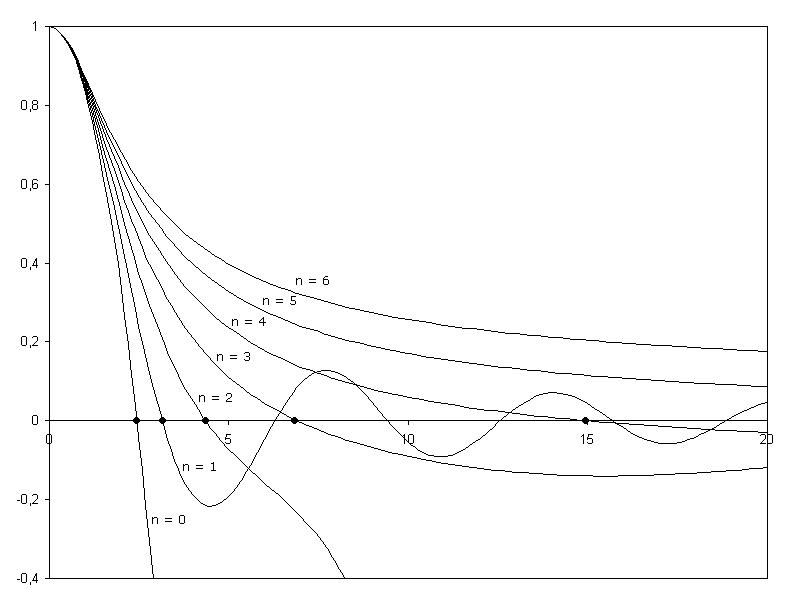
\includegraphics[width=0.75\linewidth]{Pictures/figures/Lane-emden.jpeg}
    \caption{Solutions to the Lane-Emden equation subject to the boundary conditions discussed in this section. Note the appearance of zeros in the solutions, which are representative of the truncation radius.}
    \label{fig:lane-emden}
\end{figure}
\subsection{General Properties of the Lane-Emden Equation}

It is worthwhile to study some of the very basic details of the Lane-Emden equation (equation~\ref{eq:Lane-Emden}) in order to get a feel for the sorts of solutions that arise from this problem. In general, one \textbf{needs to numerically integrate} the Lane-Emden (LE) equation in order to find solutions; however, special exceptions to this behavior exist for \framebox{$n = 0, 1, 5$.} We will study these solutions below in more detail.
\par
Before discussing solutions, we first need to discuss the \textbf{boundary conditions} for the LE equation. We are interested in solutions of the LE equation on domains characterized by the a specific \textbf{truncation radius (surface radius)} $r_T$: $D = [0,r_T] \subset \mathbb{R}$. Corresponding to this, we have $\xi \in [0,\xi_T]$; however, we \textbf{don't actually know $\xi_T$.} Instead, we recognize that, at $\xi = \xi_T$, we require that $\Theta = 0$ corresponding to \textbf{zero-density}. Thus, \framebox{$\xi_T$ is the \textbf{first zero} of the solution.}
\par
At $\xi = 0$, we need 
\[
\rho = \rho_C \Theta^n = \rho_C \implies \Theta(\xi = 0) = 1.
\]
Likewise, because $\Theta$ is a \textbf{scale-free potential}, 
\[
\frac{d\Theta}{d\xi} \propto \frac{d\Phi}{dr} = 0\;\text{by Gauss' Law.}
\]
Thus, we are interested in solving the following \textbf{Boundary Value Problem (BVP):}
\begin{equation}
\boxed{
    \frac{1}{\xi^2}\partial_\xi\left(\xi^2 \partial_\xi \Theta\right)  - \Theta^n = 0\;\; \text{where}\;\;\xi \in [0, \xi_T],\; \Theta(0) = 1,\; \Theta'(0) = 0.}
\end{equation}

We will now discuss specific solutions which are analytically known.

\subsubsection{The $n=0$ Solution}

For $n=0$, the LE equation takes the form
\begin{equation}
    \partial_\xi \left(\xi^2 \partial_\xi \Theta\right) = - \xi^2,
\end{equation}
which can be integrated once in the form
\[
\int \frac{\partial}{\partial \xi}\left(\xi^2 \frac{\partial \Theta}{\partial \xi}\right) \;d\xi = \xi^2 \frac{\partial \Theta}{\partial \xi} = - \frac{1}{3}\xi^3 + C_0.
\]
Integrating again yields
\[
\frac{\partial \Theta}{\partial \xi} =-\frac{1}{3} \xi + C_0\xi^{-2} \implies \Theta = -\frac{1}{6}\xi^2 - \frac{C_0}{\xi} + C_1.
\]
In order to \textbf{avoid asymptotic behavior} as $\xi \to 0$, we need $C_0 = 0$. Likewise, at $\xi = 0$, we need $C_1 = 1$ to match our boundary conditions. Therefore,
the solution is
\begin{equation}
\label{eq:solution_n1_le}
    \boxed{
    \Theta(\xi) = 1 - \frac{1}{6}\xi^2.
    }
\end{equation}
\par
The boundary occurs at the first $\Theta = 0$, which occurs at $\xi_T = \sqrt{6}$. 

\subsubsection{The $n=1$ Solution}

For the $n=1$ case, we have 
\[
\frac{1}{\xi^2} \frac{\partial }{\partial \xi}\left(\xi^2 \frac{\partial \Theta}{\partial \xi}\right) = \frac{\partial^2 \Theta}{\partial \xi^2} + \frac{2}{\xi} \frac{\partial \Theta}{\partial \xi} + \Theta = 0.
\]
We solve this by \textbf{power-law methods}: consider a solution
\[
\Theta(\xi) = \sum_{n=0}^\infty \alpha_n \xi^n,
\]
then
\[
\sum_{n=0}^\infty (n+2)(n+1) \alpha_{n+2} \xi^{n} \;+ \sum_{n=0}^\infty 2(n+2) \alpha_{n+2} \xi^n + \sum_{n=0}^\infty \alpha_n \xi^n = 0.
\]
Equating terms, we find
\[
(n+2)(n+3) \alpha_{n+2} + \alpha_n = 0 \implies \alpha_{n+2} = \frac{\alpha_n}{(n+2)(n+3)}.
\]
If we start from some $\alpha_0$, then
\[
\alpha_{2k} = \frac{(-1)^k}{(2k +1)!}\alpha_0.
\]
We could do the same for the odd elements, but we recognize that $\alpha_1 = 0$ by our boundary conditions. A quick look at a Taylor-Series table shows that this power law corresponds to 
\[
\Theta(\xi) \sim \alpha_0 \frac{\sin \xi}{\xi}.
\]
To maintain the boundary condition, we have
\begin{equation}
    \Theta(\xi) = \frac{\sin \xi}{\xi}.
\end{equation}
Clearly, in this case, \framebox{$\xi_T = \pi$.}
\begin{remark}
    This is actually even easier with the substitution $\chi = \Theta \xi$, in which case the equation takes the form
    \[
    \frac{d^2\chi}{d\xi^2} = - \chi^n/\xi^{n-1}.
    \]
    which is a simple second order ODE.
\end{remark}

\subsubsection{The $n=5$ Solution}

We start from the Lane Emden equation:
\begin{equation}
    \frac{1}{\xi^{2}} \frac{d}{d\xi} \left(\xi^{2} \frac{d\theta}{d\xi}\right) + \theta^{5} = 0.
\end{equation}

Rewriting for the derivative $\tfrac{d\theta}{d\xi}$ produces
\begin{equation}
    \frac{d\theta}{d\xi} 
    = \frac{1}{2}\left(1+\frac{\xi^{2}}{3}\right)^{3/2} \cdot \frac{2\xi}{3}
    = \frac{\xi}{3}\left(1+\frac{\xi^{2}}{3}\right)^{-3/2}.
\end{equation}

Differentiating again with respect to $\xi$ leads to
\begin{equation}
    \theta^{5}
    = \frac{\xi^{2}}{\left(1+\frac{\xi^{2}}{3}\right)^{3/2}}
    + \frac{3\xi^{2}}{9\left(1+\frac{\xi^{2}}{3}\right)^{5/2}}
    = \frac{9}{9\left(1+\frac{\xi^{2}}{3}\right)^{5/2}}.
\end{equation}

This reduces to
\begin{equation}
    \theta^{5} = \frac{1}{\left(1+\frac{\xi^{2}}{3}\right)^{5/2}}.
\end{equation}

Therefore, the Lane--Emden equation has the analytic solution
\begin{equation}
    \theta(\xi) = \frac{1}{\sqrt{1+\xi^{2}/3}}, \qquad n=5.
\end{equation}

This solution corresponds to a configuration of finite mass but infinite radial extent. 

\subsection{Scaling Relations of the Lane-Emden Equation}

We \textbf{cannot generally solve} the Lane-Emden equation; however, we can derive various scaling relationships between the relevant quantities in the equations. This is useful as it can tell us (\textbf{for fixed $n$}) how certain properties scale with one another. The core of this idea is that \textit{regardless of scaling}, $\Theta_n(\xi)$ is a \textbf{fixed function for each index}. As such, different physical solutions for the same $n$ are forced to have similar properties.
\par
Assume that we have, by numerical integration or otherwise, obtained a solution $\Theta(\xi)$ for a particular index $n$. we know that $\xi$ and $\Theta$ are defined (see equation~\ref{eq:LE-length} and \eqref{eq:LE-density}) such that
\[
    \xi = \left(\frac{4\pi G \rho_C}{\Phi_T-\Phi_C}\right)^{1/2} r = \alpha r,
\]
and
\[
\rho = \rho_C \Theta^n,\;\rho_C = \left(\frac{\Phi_T-\Phi_C}{(n+1)K}\right)^n.
\]
Substituting the expression for $\rho_C$ into $\alpha$, we find that
\begin{equation}
    \boxed{
    \xi = \left(\frac{4\pi G \rho_C^{1-(1/n)}}{K(n+1)}\right)^{1/2}r,
    }
\end{equation}
which gives us an exact scaling on the \textbf{maximum radius} in terms of the \textbf{core density}:
\begin{equation}
    \label{eq:LE-scaling-radius}
    R_{\rm max} = \alpha \xi_{T} \propto \rho_C^{(n-1)/2n}.
\end{equation}
\par
We may also then ask about the scaling of the total mass with the core density and the radius. Clearly, if 
\[
\rho \sim \rho_C \Theta^n, \implies M = 4\pi \rho_C \alpha^{-3} \int_0^{\xi_T}\;d\xi \;\Theta^n \xi^2 \propto \rho_C \alpha^{-3}. 
\]
Since $\alpha \sim \rho_C^{(n-1)/2n}$, we know that
\[
M \sim \rho_C \rho_C^{-3(n-1)/2n} = \rho_c^{(3-n)/2n}
\]
Comparing this to the scaling for $R$, we have
\[
M \sim R^{(3-n)/(1-n)}.
\]

\subsection{Bonnor-Ebert Spheres}

When \( n = \infty \), we obtain the \textbf{isothermal equation of state}, 
\[
P = K \rho,
\]
which implies
\[
K \nabla \log \rho = \nabla \Phi \quad \Rightarrow \quad \rho = \rho_0 \exp\left(-\frac{\Phi - \Phi_0}{K}\right).
\]
Substituting this relation into the Poisson equation,
\[
\nabla^2 \Phi = 4\pi G \rho,
\]
we obtain:
\[
\nabla^2 \Phi = 4\pi G \rho_0 \exp\left(-\frac{\Phi - \Phi_0}{K}\right).
\]
Now, define a dimensionless potential:
\[
\psi \equiv \frac{\Phi - \Phi_0}{K}, \quad \text{so that} \quad \rho = \rho_0 e^{-\psi}.
\]
Then the equation becomes:
\[
\nabla^2 \psi = \frac{4\pi G \rho_0}{K} e^{-\psi}.
\]

To nondimensionalize, define a radial coordinate:
\[
\xi \equiv \frac{r}{r_0}, \quad \text{with} \quad r_0^2 = \frac{K}{4\pi G \rho_0}.
\]
Then the Laplacian in spherical symmetry becomes:
\[
\frac{1}{r^2} \frac{d}{dr} \left( r^2 \frac{d\psi}{dr} \right)
= \frac{1}{r_0^2 \xi^2} \frac{d}{d\xi} \left( \xi^2 \frac{d\psi}{d\xi} \right).
\]
Thus, the final form of the \textbf{isothermal Lane–Emden equation} is:
\[
\boxed{
\frac{1}{\xi^2} \frac{d}{d\xi} \left( \xi^2 \frac{d\psi}{d\xi} \right) = e^{-\psi}.
}
\]
This is the equation that governs the structure of the \textbf{isothermal sphere}. 

\subsubsection{Bonnor-Ebert Spheres}

Assume a power-law behavior for the density at large \( \xi \),
\[
\rho(\xi) \propto \xi^{-n} \quad \Rightarrow \quad \psi(\xi) = n \log \xi + \text{const}.
\]

Then compute derivatives:
\[
\frac{d\psi}{d\xi} = \frac{n}{\xi}, \qquad \frac{d^2\psi}{d\xi^2} = -\frac{n}{\xi^2}.
\]

Substitute into the left-hand side of the equation:
\[
\frac{d^2\psi}{d\xi^2} + \frac{2}{\xi} \frac{d\psi}{d\xi} = -\frac{n}{\xi^2} + \frac{2n}{\xi^2} = \frac{n}{\xi^2}.
\]

On the right-hand side:
\[
e^{-\psi} = e^{-n \log \xi + \text{const}} = C \cdot \xi^{-n}.
\]
To be consistent, both sides must scale the same way, so:
\[
\frac{n}{\xi^2} \propto \xi^{-n} \quad \Rightarrow \quad n = 2.
\]

\begin{tcolorbox}[colback=blue!5!white, colframe=blue!75!black, title=Asymptotic Form]
At large radii, the solution to the isothermal Lane-Emden equation behaves as:
\[
\boxed{
\rho(\xi) \propto \xi^{-2}, \qquad \psi(\xi) \sim 2 \log \xi + \text{const}.
}
\]
This is the familiar result for the singular isothermal sphere.
\end{tcolorbox}

Here's the problem: \textbf{this means the mass is infinite}. So what happens if we instead force the system to truncate at a particular radius $r_t$? In that case, we need to introduce an \textbf{external pressure source} in order to make up for the missing gravitational mass. Since $P = K \rho$, we can simply say that
\[
P_{\rm ext} = K \rho(r_T).
\]
\subsubsection{Stability of Bonnor–Ebert Spheres}

A natural question is: \textbf{what happens when we perturb the truncation radius $r_T$ slightly}? For instance, a small compression of the sphere might result from infalling material, a shock, or some internal perturbation. The key diagnostic is the response of the required external pressure $P_{\rm ext}$. If $P_{\rm ext}$ increases to oppose the compression, the configuration is stable; if $P_{\rm ext}$ decreases, the configuration is unstable and the collapse may run away.

We consider a family of truncated isothermal spheres with central density $\rho_c$, truncated at radius $r_T$, and held in equilibrium by an external pressure $P_{\rm ext}$. From the isothermal Lane–Emden solution, we define:

\begin{itemize}
    \item The dimensionless radius: $\xi = r / R_0$, where $R_0^2 = \alpha / (4\pi G \rho_c)$,
    \item The dimensionless potential: $\psi(\xi)$ such that $\rho(\xi) = \rho_c e^{-\psi(\xi)}$,
    \item The \textbf{mass function} (not the actual mass!):
    \[
    m(\xi) = \xi^2 \frac{d\psi}{d\xi}.
    \]
\end{itemize}

Then, the pressure at the outer boundary is
\[
P_{\rm ext} = K\rho(\xi_T) = K\rho_c e^{-\psi(\xi_T)}.
\]

We now vary $\xi_T$ slightly and track the behavior of $P_{\rm ext}$. Taking the derivative:
\[
\frac{dP_{\rm ext}}{d\xi_T} = - K \rho_c e^{-\psi(\xi_T)} \frac{d\psi}{d\xi_T}.
\]
This shows that the sign of $dP_{\rm ext}/d\xi_T$ \textbf{depends entirely on the slope $d\psi/d\xi_T$ at the boundary.}

From the Lane–Emden equation:
\[
\frac{1}{\xi^2} \frac{d}{d\xi}\left( \xi^2 \frac{d\psi}{d\xi} \right) = e^{-\psi},
\]
we can numerically solve for $\psi(\xi)$ and its derivatives. One then computes $dP_{\rm ext}/d\xi_T$ and finds that:

\begin{itemize}
    \item For $\xi_T < \xi_{\rm crit} \approx 6.451$, the derivative is negative: compressing the sphere increases $P_{\rm ext}$, which resists the compression. This implies \textbf{stability}.
    \item For $\xi_T > \xi_{\rm crit}$, the derivative is positive: compressing the sphere decreases $P_{\rm ext}$, which fails to resist collapse. This implies \textbf{instability}.
\end{itemize}

Thus, the function $P_{\rm ext}(\xi_T)$ reaches a minimum at $\xi_T = \xi_{\rm crit}$. Beyond this point, the configuration cannot remain in equilibrium without fine-tuned external support. Thus, the Bonnor–Ebert sphere provides a natural \textbf{threshold model for gravitational collapse}.

\begin{tcolorbox}[colback=red!5!white, colframe=red!75!black, title=Bonnor–Ebert Stability Criterion]
A Bonnor–Ebert sphere is:
\begin{itemize}
    \item \textbf{Stable} if $\xi_T < \xi_{\rm crit} \approx 6.451$,
    \item \textbf{Unstable} if $\xi_T > \xi_{\rm crit}$.
\end{itemize}
The instability corresponds to collapse under self-gravity once external pressure support becomes insufficient.
\end{tcolorbox}

\subsection{Implications of Polytropic Models and Bonnor–Ebert Spheres}

Polytropic models provide a powerful, unifying framework for understanding the structure of self-gravitating astrophysical objects under hydrostatic equilibrium. The simplicity of the polytropic equation of state,
\[
P = K \rho^{1 + 1/n},
\]
permits analytic and semi-analytic solutions to otherwise intractable stellar structure problems. Their implications span a wide range of astrophysical scenarios:

\begin{enumerate}
    \item \textbf{Unified Treatment of Stellar Interiors} \\
    Many types of stars — from low-mass dwarfs to massive stars — are approximately modeled by different polytropic indices. For example:
    \begin{itemize}
        \item Fully convective stars $\rightarrow$ $n \approx 1.5$,
        \item Degenerate cores or white dwarfs $\rightarrow$ $n \approx 1.5$ (non-relativistic) or $n = 3$ (ultrarelativistic),
        \item Radiation-pressure dominated massive stars $\rightarrow$ $n \rightarrow 3$.
    \end{itemize}
    This enables comparison across different evolutionary stages and mass regimes.

    \item \textbf{Insights into Stellar Stability and Limits} \\
    The solutions to the Lane–Emden equation for various $n$ reveal key stability properties. For instance, polytropes with $n < 5$ have finite radius and mass, while those with $n \geq 5$ are unbounded. This connects directly to phenomena like the Chandrasekhar mass limit and the onset of instability in massive stars.

    \item \textbf{Analytic Scaling Relations} \\
    Polytropes yield closed-form scaling laws for core pressure, density, temperature, and radius as functions of mass and composition. These relations are essential for interpreting observations and for initializing stellar evolution models.

    \item \textbf{Bonnor–Ebert Spheres as Collapse Thresholds} \\
    The isothermal limit ($n = \infty$) leads to the Bonnor–Ebert sphere: a pressure-confined, self-gravitating equilibrium solution. This model provides a physically motivated criterion for gravitational instability in interstellar gas:
    \begin{itemize}
        \item For $\xi_T < \xi_{\rm crit} \approx 6.451$, the configuration is stable.
        \item For $\xi_T > \xi_{\rm crit}$, small perturbations lead to runaway collapse.
    \end{itemize}
    Observed molecular cloud cores that match the radial density profiles of Bonnor–Ebert spheres can be diagnosed as collapsing or stable depending on their dimensionless radius.

    \item \textbf{Connection to Star Formation} \\
    Bonnor–Ebert spheres offer one of the few analytic, observationally testable models for the initial stages of star formation. They predict the critical conditions — mass, temperature, external pressure — under which a prestellar core transitions from quasi-static equilibrium to gravitational collapse.

    \item \textbf{Bridge Between Microphysics and Macrophysics} \\
    Polytropic models illustrate how microphysical assumptions (e.g., ideal gas law, radiation pressure, degeneracy) manifest as macroscopic structure. The mapping from $n$ to physical processes connects thermodynamics, radiative transport, and hydrodynamics in a compact formalism.

\end{enumerate}

\section{The Intracluster Medium}

Galaxy clusters are composed of several mass components, approximately partitioned as:
\begin{itemize}
    \item \textbf{Dark Matter} — $\sim 85\%$
    \item \textbf{Hot Ionized Gas (Intracluster Medium)} — $\sim 14\%$
    \item \textbf{Stars in Galaxies} — $\sim 1\%$
\end{itemize}

The \textbf{intracluster medium (ICM)} is a hot ($T \sim 10^7$–$10^8$ K), diffuse plasma that emits strongly in the X-ray band via thermal bremsstrahlung and line emission. The X-ray surface brightness and spectral information allow observers to reconstruct the projected temperature and density profiles of the gas.

\subsection{Hydrostatic Equilibrium in the ICM}

For a galaxy cluster in approximate \textbf{hydrostatic equilibrium}, the pressure gradient in the ICM must balance the gravitational force from the total mass:
\[
\frac{dP}{dr} = -\rho_g(r) \frac{d\Phi}{dr},
\]
where:
\begin{itemize}
    \item $P(r)$ is the gas pressure,
    \item $\rho_g(r)$ is the gas density,
    \item $\Phi(r)$ is the total gravitational potential sourced by all mass components: dark matter, stars, and gas.
\end{itemize}

The pressure of the gas is related to its density and temperature by the ideal gas law:
\[
P(r) = \frac{k_B}{\mu m_p} \rho_g(r) T(r) \equiv K \rho_g(r) T(r),
\]
where:
\begin{itemize}
    \item $k_B$ is Boltzmann’s constant,
    \item $m_p$ is the proton mass,
    \item $\mu$ is the mean molecular weight (typically $\mu \approx 0.6$),
    \item $T(r)$ is the radial temperature profile.
\end{itemize}

\subsection{General Expression for the Dynamical Mass}

Applying the product rule and dividing by $\rho_g$, the hydrostatic balance becomes:
\[
\frac{1}{\rho_g} \frac{dP}{dr} = K \frac{dT}{dr} + K T \frac{d\log \rho_g}{dr} = -\frac{d\Phi}{dr}.
\]
The gravitational acceleration is related to the total enclosed mass $M_{\rm dyn}(<r)$ via:
\[
\frac{d\Phi}{dr} = \frac{G M_{\rm dyn}(<r)}{r^2}.
\]
Combining these gives:
\[
K \left( \frac{dT}{dr} + T \frac{d\log \rho_g}{dr} \right) = -\frac{G M_{\rm dyn}(<r)}{r^2}.
\]
Dividing both sides by $K$ and rearranging, we find the key relation for the enclosed dynamical mass:
\begin{tcolorbox}[colback=blue!5!white, colframe=blue!75!black, title=Hydrostatic Mass Equation for the ICM]
\begin{equation}
\boxed{
M_{\rm dyn}(<r) = -\frac{r^2}{G} \frac{k_B T(r)}{\mu m_p} \left[ \frac{d\log T}{dr} + \frac{d\log \rho_g}{dr} \right].
}
\end{equation}
\end{tcolorbox}

This expression allows observers to estimate the total (mostly dark) mass of a cluster using observed profiles of $T(r)$ and $\rho_g(r)$ under the assumption of hydrostatic equilibrium. It is widely used in X-ray and SZ studies of galaxy clusters.

\subsection{Limitations and Caveats}

\begin{itemize}
    \item The ICM is \textbf{not truly isothermal}; real temperature profiles typically decline at large radii.
    \item Non-thermal pressure support (e.g., turbulence, magnetic fields, cosmic rays) can cause hydrostatic mass estimates to \textbf{underestimate} the true mass.
    \item This method assumes \textbf{spherical symmetry} and \textbf{equilibrium}, which may be violated in merging or dynamically active clusters.
\end{itemize}


\chapter{Sound Waves}
In this section, we'll discuss the propogation of waves in fluids. In many ways, this is reminiscent of the exercise as it is typically introduced in thermodynamics; however, we will instead formally derive the relevant wave equations and show how the behaviors differ in different scenarios.

This section will primarily utilize \textbf{first-order perturbation theory} to explore what happens when we perturb a fluid dynamic system from equilibrium. These perturbations can generate a number of very fascinating phenomena, which, which coupled with various other forces, generate a whole host of wave types relevant in astrophysics:
\vspace{0.5cm}
\begin{table}[h!]
\centering
\caption{Common fluid waves in astrophysical contexts.}
\begin{tabular}{l p{5cm} p{5cm}}
\hline
\textbf{Wave Type} & \textbf{Cause / Restoring Force} & \textbf{Astrophysical Relevance} \\
\hline
Sound waves & Pressure gradients (compressibility of gas) & Transport of information and energy; stability of stellar interiors; shocks in ISM and IGM. \\
Gravity waves (internal) & Buoyancy in stably stratified media & Mixing and transport in stellar interiors; oscillations in neutron stars; atmospheric waves in planets. \\
Surface gravity waves & Gravity acting at fluid interfaces & Oscillations on stellar surfaces; accretion disk boundaries; star–planet interactions. \\
Inertial waves & Coriolis force due to rotation & Differential rotation and turbulence in stars and planets; angular momentum transport in disks. \\
Magnetosonic waves & Combination of pressure gradients and magnetic tension & Propagation of perturbations in magnetized plasmas; shocks in solar wind; structure of jets. \\
Alfvén waves & Magnetic tension alone & Energy transport in magnetized plasmas; coronal heating; particle acceleration in solar and stellar winds. \\
Kelvin–Helmholtz waves & Shear across a fluid interface & Mixing in stellar winds and jets; interface instabilities in accretion flows. \\
\hline
\end{tabular}
\end{table}
\vspace{0.5cm}

\section{Elements of Perturbation Theory}

The method of perturbations provides a systematic way to study the response of a fluid system to \textbf{small deviations from equilibrium}.  Rather than attempting to solve the full nonlinear fluid equations, we expand the relevant quantities in small deviations from a known background solution.  
Depending on the nature of the perturbation, the system may exhibit one of two broad behaviors:
\vspace{0.25cm}
\begin{itemize}
    \item \textbf{Oscillatory response:} the perturbation remains bounded and typically corresponds to wave–like motion or stable oscillations.
    \item \textbf{Instability:} the perturbation grows with time, often leading to a qualitative change in the system (e.g. turbulence, collapse, or fragmentation).
\end{itemize}
\vspace{0.25cm}
Formally, we introduce a small parameter $\epsilon \ll 1$ that measures the size of the perturbation relative to the background.  
If $\psi(x,t)$ is a known equilibrium solution, we expand the perturbed solution as
\[
\psi'(x,t) = \psi(x,t) + \epsilon \psi_1(x,t) + \epsilon^2 \psi_2(x,t) + \cdots.
\]
Substituting into the governing PDE and collecting terms of equal order in $\epsilon$ yields a hierarchy of equations.  
At first order, the \textbf{governing equation is linear in $\psi_1$, justifying the term \emph{linear perturbation theory}.}


\subsection{Fluid Perturbations}

As we have discussed in chapter~\ref{ch:1}, there are two perspectives on fluid dynamics: the \textbf{Lagrangian} and the \textbf{Eulerian} frameworks. Just as we can describe any \textbf{fluid field} $\psi$ in either it's Lagrangian form or its Eulerian form, we can likewise describe perturbations in a field in either an Eulerian formalism or a Lagrangian formalism. As we will see throughout this section, the distinction can be extremely important depending on what sort of problem you seek to solve.
\par
Recall from definitions~\ref{def:Eulerian} and~\ref{def:Lagrangian} that a physical quantity \( \psi \) (e.g., density, pressure, velocity) may be expressed as either
\[
\begin{aligned}
    \textbf{Eulerian:} \quad & \psi_{\rm Euler}(\mathbf{x}, t) := \psi_{\rm Lagrangian}(\boldsymbol{\varphi}^{-1}({\bf x},t),t), \\
    \textbf{Lagrangian:} \quad & \psi_{\rm Lagrangian}(\mathbf{X}, t) := \psi_{\rm Euler}(\boldsymbol{\varphi}(\mathbf{X}, t), t),
\end{aligned}
\]
where \( \mathbf{X} \in \mathcal{C}_0 \) is the material label of a fluid particle (i.e., its position in the reference configuration), and \( \boldsymbol{\varphi} \) is the \textbf{flow map} that gives the current position \( \mathbf{x} \in \mathcal{C}_t \) of that particle at time \( t \).
\par
Let us now consider a fluid in equilibrium $(\rho_0,P_0, {\bf u}_0)$. We may introduce a perturbation to these fields in a physical sense; however, just as the underlying fields may be described in either framework, so too can the perturbations:
\vspace{0.5cm}
\begin{definition}[Eulerian perturbation]
Let \( \psi(\mathbf{x},t) \) be a fluid field (e.g., density, pressure, velocity) and let \( \psi_0(\mathbf{x}) \) denote its equilibrium value at the same spatial point.  The \textbf{Eulerian perturbation} is defined by
\[
\delta \psi(\mathbf{x},t) := \psi(\mathbf{x},t) - \psi_0(\mathbf{x}).
\]
That is, the Eulerian perturbation measures the instantaneous departure of the field 
from equilibrium at a fixed position in space.
\par
This is, perhaps, the more intuitive of the two: you imagine performing the same fluid flow experiment side by side with marginally different initial conditions. You then measure the perturbation as the \textbf{different between the flows at a given point}.
\end{definition}
\vspace{0.5cm}
\begin{definition}[Lagrangian perturbation]
Let \( \mathbf{X} \) denote the material label of a fluid element in the reference configuration, and let \( \boldsymbol{\varphi}(\mathbf{X},t) \) be the associated flow map that gives the current position \( \mathbf{x} = \boldsymbol{\varphi}(\mathbf{X},t) \).The Lagrangian perturbation of a field is defined as
\[
\Delta \psi(\mathbf{X},t) := \psi(\boldsymbol{\varphi}(\mathbf{X},t),t) - \psi_0(\mathbf{X}).
\]
That is, the Lagrangian perturbation measures the departure of the field experienced by a moving fluid element relative to its equilibrium value.
\par
This is the more difficult quantity to measure. We imagine again running two near identical fluid experiments and labeling the same fluid element in each of the experiments based on the initial configuration. When we run the experiments, the \textbf{Lagrangian Perturbation} measures the difference between the \textbf{two different fluid elements}.
\end{definition}
\vspace{0.5cm}
As such, we really need to assess what we are trying to describe / measure in our computations. The Eulerian perturbation is perhaps easier to measure, but it suffers from the fact that a particular fluid element in one experiment will not generally end up in the same place later on as it does in a second experiment. This is the realm of the Lagrangian perturbation, which is really concerned with the differing experiences of the particles in a given fluid element.

\subsubsection*{Converting Between Frames}

Let's look now at the connection between Eulerian and Lagrangian perturbations. We imagine two fluid experiments: in one, we have a quasi-stable equilibrium described by fluid fields $(\rho_0,P_0,{\bf u}_0).$ In the other, we have the same system subjected to a perturbation:
\[
(\rho_0,P_0,{\bf u}_0) \to (\rho_0 + \delta \rho,P_0+\delta P, {\bf u}_0 + \delta {\bf u}).
\]
\par
In the \textbf{unperturbed flow}, a particular fluid element ${\bf X}$ (Lagrangian frame) will move through space as determined by the \textbf{flow map} $\boldsymbol{\varphi}({\bf X},t)$. We can describe how far that fluid element has gone by
\[
\boldsymbol{\xi}({\bf X},t) = \boldsymbol{\varphi}({\bf X},t) - \boldsymbol{\varphi}({\bf X},0) = \boldsymbol{\varphi}({\bf X},t) - {\bf X}.
\]
This is the so-called \textbf{displacement field}: it tells us how far away a particular fluid element is from its starting position. Let's consider the perturbed flow. Clearly there will be a slightly different flow map $\boldsymbol{\vartheta}$ and subsequently a slightly different displacement field $\boldsymbol{\varrho}$ such that
\[
\boldsymbol{\varrho}({\bf X},t) = \boldsymbol{\vartheta}({\bf X},t) - {\bf X}.
\]
Let's now ask the following question: \textbf{what are the perturbations we measure?} Consider a field $\psi$ of the flow. For a particular position in space and time $({\bf X},t)$, the \textbf{Eulerian perturbation} will be
\[
\delta \psi({\bf x},t) = \psi({\bf x},t) - \psi_0({\bf x},t).
\]
What happens to the \textbf{Lagrangian Perturbation}? Well that is
\[
\Delta \psi({\bf X},t) = \underbrace{\psi(\boldsymbol{\vartheta}({\bf X},t),t)}_{\text{New field @ new location}} - \underbrace{\psi_0(\boldsymbol{\varphi}({\bf X},t),t)}_{\text{Old field @ old location}}.
\]
We can make the relation between $\delta\psi$ and $\Delta\psi$ precise by Taylor-expanding the perturbed flow about the unperturbed one.  Write
\[
\boldsymbol{\vartheta}({\bf X},t) = \boldsymbol{\varphi}({\bf X},t) 
+ \boldsymbol{\eta}({\bf X},t),
\]
where 
\[
\boldsymbol{\eta}({\bf X},t) := \boldsymbol{\varrho}({\bf X},t) - \boldsymbol{\xi}({\bf X},t)
\]
is the \emph{perturbative displacement}: the difference between the two trajectories for the same material element ${\bf X}$.

Substituting into the Lagrangian perturbation,
\[
\Delta \psi({\bf X},t) 
= \psi(\boldsymbol{\varphi}({\bf X},t) + \boldsymbol{\eta}({\bf X},t),t)
- \psi_0(\boldsymbol{\varphi}({\bf X},t),t).
\]

Now expand the first term about $\boldsymbol{\varphi}({\bf X},t)$:
\[
\psi(\boldsymbol{\varphi}+\boldsymbol{\eta},t)
= \psi(\boldsymbol{\varphi},t) 
+ \boldsymbol{\eta}\cdot\nabla\psi(\boldsymbol{\varphi},t) 
+ \mathcal{O}(|\boldsymbol{\eta}|^2).
\]

Hence,
\[
\Delta \psi({\bf X},t) 
= \underbrace{\big[\psi(\boldsymbol{\varphi},t)-\psi_0(\boldsymbol{\varphi},t)\big]}_{\delta\psi(\boldsymbol{\varphi},t)}
+ \boldsymbol{\eta}\cdot\nabla \psi_0(\boldsymbol{\varphi},t)
+ \mathcal{O}(|\boldsymbol{\eta}|^2).
\]

To first order, we therefore obtain the fundamental relation
\begin{equation}
    \label{eq:convert_perturbs}
    \boxed{ \ \Delta \psi = \delta \psi + \boldsymbol{\eta}\cdot\nabla\psi_0 \ }.
\end{equation}
\begin{remark}
    For those well versed in differential geometry, this is precisely the \textbf{Lie Derivative}. Additionally, we should mention that for a static background $\boldsymbol{\eta} = \boldsymbol{\varrho}$.
\end{remark}

\begin{bigidea}
There are two ways to compare perturbed and unperturbed flows:

\begin{itemize}
    \item In the \textbf{Eulerian frame}, we stay at the same point in space 
    and measure how the field changes there:
    \[
    \delta \psi(\mathbf{x},t) = \psi(\mathbf{x},t) - \psi_0(\mathbf{x},t).
    \]

    \item In the \textbf{Lagrangian frame}, we follow a given fluid element along its trajectory 
    and compare what it experiences in the perturbed vs.\ unperturbed flow:
    \[
    \Delta \psi(\mathbf{X},t) = \psi(\boldsymbol{\vartheta}(\mathbf{X},t),t) 
    - \psi_0(\boldsymbol{\varphi}(\mathbf{X},t),t).
    \]
\end{itemize}

The key difference is thus:  
\emph{Eulerian perturbations compare fields at the same location,  while Lagrangian perturbations compare fields along the same material element’s path.}

\[
\boxed{\;\Delta \psi \;=\; \delta \psi \;+\; \boldsymbol{\eta}\cdot\nabla \psi_0 \;}
\]

Here $\boldsymbol{\eta}$ is the perturbative displacement (the difference between the perturbed and unperturbed trajectories).  
This conversion formula is the workhorse for translating between the two perspectives.
\end{bigidea}

\section{The General Approach}

Fluids possess two key physical properties: they can \emph{transmit momentum} through internal stresses, and they can \emph{oscillate about an equilibrium configuration} when displaced. These features make them natural hosts for a wide variety of wave phenomena. In fluid dynamics, the systematic study of such phenomena is most effectively carried out using \textbf{first-order perturbation theory}, in which small deviations from an established equilibrium state are introduced and their subsequent evolution is analyzed.

\subsection*{The Equilibrium Configuration}

The first step in any perturbative analysis is to specify the equilibrium state of the system. In the present context, this corresponds to a hydrostatic configuration in which the velocity field vanishes, ${\bf u} = 0$, and the pressure and density take prescribed background forms, $p = p_0({\bf x})$ and $\rho = \rho_0({\bf x})$. All subsequent perturbations will be defined relative to this reference state.

\begin{remark}
    As we will see, the spatial structure of the equilibrium configuration can strongly influence both the types of waves that can exist and the manner in which they propagate through the medium.
\end{remark}

\subsection*{The Perturbation}

With the equilibrium configuration specified, we are able to introduce a perturbation to that original configuration. One can choose to either view that perturbation in the Lagrangian framework or the Eulerian one (\rmk{it is important to remember that ANY perturbation is BOTH Eulerian and Lagrangian depending on how you choose to view it}). For need of a choice, we'll use the \textbf{Eulerian} ($\delta$) perturbation here, but as will be explored below, the relevant equations may be derived from either framework. Thus, our perturbed fields introduce a new \textbf{initial boundary value problem (IBVP)} with initial conditions
\begin{equation}
    \begin{aligned}
        \rho({\bf x},0) &= \rho_0({\bf x},0) + \delta \rho({\bf x},0)\\
        P({\bf x},0) &= P_0({\bf x},0) + \delta P({\bf x},0)\\
       {\bf u}({\bf x},0) &= \delta {\bf u}({\bf x},0).
    \end{aligned}
\end{equation}
Of course, introducing this perturbation will also change the flow map $\boldsymbol{\varphi}$ from the Lagrangian framework and the corresponding displacement fields.
\par
Our goal now is to determine the equations of motion for the flow in terms of the first order perturbations and solve them using linearization.

\subsection{The Linearized Fluid Equations}

As is the standard approach in all forms of perturbation theory, we now consider what happens to the \textbf{continuity equation} and the \textbf{Euler equation} under the assumption of linear perturbation. Let's look first at the continuity equation:
\[
\frac{\partial \rho}{\partial t} + \nabla \cdot (\rho{\bf u}) = 0.
\]
Letting $\rho \mapsto \rho_0 + \delta \rho$, etc. we have
\[
\underbrace{\frac{\partial \rho_0}{\partial t}}_{\text{0 by HSE}} + \frac{\partial \delta \rho}{\partial t} + \nabla \cdot \left(\rho_0\delta{\bf u}+ \underbrace{\delta \rho \delta {\bf u}}_{\text{2nd order}}\right) = 0,
\]
which takes the linearized form
\begin{equation}
    \label{eq:linear_continuity_euler}
    \boxed{
    \frac{\partial \delta \rho}{\partial t} + \nabla \cdot(\rho_0 {\bf \delta u}) = 0.
    }
\end{equation}
In the \textbf{Lagrangian} approach, inserting our perturbation (\rmk{In the LAGRANGIAN form}),
\[
\frac{D(\rho_0 + \Delta \rho)}{Dt} + (\rho_0 + \Delta \rho) \nabla \cdot {\bf u{}} = 0 .
\]
Keeping \textbf{only first order terms} and recognizing that ${\bf u} = \partial_t \boldsymbol{\xi}$,
\begin{equation}
    \label{eq:linear_continuity_lagrangian}
    \boxed{
    \frac{D\Delta \rho}{Dt} + \rho_0 \nabla \cdot \partial_t \boldsymbol{\xi} = 0.
    }
\end{equation}
\par
We now look at the \textbf{Euler Equation}. Assuming the situation to be inviscid, we have
\[
\rho \frac{\partial {\bf u}}{\partial t} + \rho {\bf u} \cdot \nabla {\bf u} = -\nabla P+ \rho{\bf f}_{\rm ext}.
\]
In the context of our perturbative expansion, we can eliminate higher order terms to find
\[
\rho_0 \frac{\partial \delta {\bf u}}{\partial t} = \underbrace{-\nabla P_0 + \rho_0{\bf f}_{\rm ext}}_{\text{=0 by HSE}} - \nabla \delta P + \delta \rho {\bf f}_{\rm ext}.
\]
Thus, the \textbf{linearized Euler's Equation} is
\begin{equation}
    \label{eq:euler_linearized_eulerian}
    \boxed{
    \frac{\partial \delta {\bf u}}{\partial t} = - \frac{\nabla \delta P}{\rho_0} + \frac{\delta \rho}{\rho_0} {\bf f}_{\rm ext}.}
\end{equation}
In the Lagrangian framework,
\[
\frac{D\Delta {\bf u}}{Dt} = \frac{1}{\rho_0} \left[\Delta \rho {\bf f}_{\rm ext} - \nabla \Delta P\right].
\]
Notably, remember that ${\bf u} = \Delta {\bf u} = \partial_t \boldsymbol{\xi}$. Additionally, $\partial_t \boldsymbol{\xi} \sim D_t\boldsymbol{\xi}$ to first order. Thus,
\begin{equation}
\label{eq:euler_linearized_lagrangian}
\boxed{
\frac{\partial^2 \boldsymbol{\xi}}{\partial t^2} = \frac{1}{\rho_0} \left[\Delta \rho {\bf f}_{\rm ext} - \nabla \Delta P \right]}
\end{equation}
With these, we now have the fully linearized equations for our fluid flow problems.

\subsection{The Wave Equation}

We now derive the wave equation for small perturbations of a barotropic fluid,  working in the Lagrangian formalism introduced above and then in the Eulerian formalism.

\subsubsection*{The Lagrangian Wave Equation}

Starting from the linearized Euler and continuity equations in Lagrangian form, 
the structure of a wave equation quickly emerges. Taking the divergence of the 
linearized Euler equation gives
\[
\nabla \cdot \left(\rho_0 \frac{\partial^2 \boldsymbol{\xi}}{\partial t^2}\right) 
= \rho_0 \nabla\cdot\left(\frac{\partial^2\boldsymbol{\xi}}{\partial t^2}\right) 
+ \frac{\partial^2\boldsymbol{\xi}}{\partial t^2} \cdot \nabla \rho_0
= - \nabla^2 \Delta p + \nabla \cdot (\Delta \rho\, {\bf f}_{\rm ext}).
\]
Meanwhile, taking the material derivative of the linearized continuity equation yields
\[
\frac{\partial ^2 \Delta \rho}{\partial t^2} 
+ \rho_0 \nabla \cdot \frac{\partial ^2\boldsymbol{\xi}}{\partial t^2} = 0.
\]
Combining these two results eliminates the divergence of $\partial_t^2 \boldsymbol{\xi}$:
\[
\frac{\partial^2 \Delta \rho}{\partial t^2} 
- \nabla^2 \Delta p 
+ \nabla \cdot (\Delta \rho\, {\bf f}_{\rm ext})
= \frac{\partial^2 \boldsymbol{\xi}}{\partial t^2} \cdot \nabla \rho_0.
\]
\textbf{For a barotropic fluid}, $p=p(\rho)$, so that
\[
dp = \frac{\partial p}{\partial \rho}\, d\rho,
\]
and therefore
\[
\Delta p = c_s^2\, \Delta \rho, \qquad
c_s^2 \equiv \frac{\partial p}{\partial \rho}.
\]
Substituting, the equation becomes
\[
\frac{\partial^2 \Delta \rho}{\partial t^2}
- \nabla^2 \!\left(c_s^2\, \Delta \rho\right)
= \frac{\partial^2 \boldsymbol{\xi}}{\partial t^2} \cdot \nabla \rho_0
- \nabla \cdot (\Delta \rho\, {\bf f}_{\rm ext}).
\]

Finally, using the Euler equation in Lagrangian form,
\[
\frac{D^2 \boldsymbol{\xi}}{Dt^2}
= \partial_t^2 \boldsymbol{\xi}
= -\frac{\nabla \Delta p}{\rho_0}
+ \frac{\Delta \rho}{\rho_0}\, {\bf f}_{\rm ext},
\]
we may write the full wave equation as
\begin{equation}
    \label{eq:lagrangian_wave_equation}
    \boxed{
    \underbrace{\frac{\partial^2 \Delta \rho}{\partial t^2} 
    - \nabla^2 \!\left(c_s^2 \Delta \rho\right)}_{\text{Classical wave operator}}
    =
    \underbrace{- \frac{\nabla \rho_0}{\rho_0} \cdot 
    \Big[\nabla \!\left(c_s^2 \Delta \rho\right) 
    - \Delta \rho\, {\bf f}_{\rm ext} \Big]}_{\text{Background coupling}}
    \;-\;
    \underbrace{\nabla \cdot \!\left(\Delta \rho\, {\bf f}_{\rm ext}\right)}_{\text{Buoyancy/external forcing}}
    }
\end{equation}
\subsubsection*{The Eulerian Wave Equation}

We can obtain an analogous wave equation directly in the Eulerian framework. Starting from the linearized continuity equation \eqref{eq:linear_continuity_euler},
\[
\frac{\partial \delta \rho}{\partial t} + \nabla \cdot \big(\rho_0 \delta \mathbf{u}\big) = 0,
\]
and the linearized Euler equation \eqref{eq:euler_linearized_eulerian},
\[
\frac{\partial \delta \mathbf{u}}{\partial t} = - \frac{\nabla \delta p}{\rho_0} 
+ \frac{\delta \rho}{\rho_0}\, \mathbf{f}_{\rm ext},
\]
we may eliminate $\delta \mathbf{u}$ to obtain a closed equation for $\delta \rho$. Taking another time derivative of the continuity equation, one finds that
\[
\frac{\partial^2 \delta \rho}{\partial t^2}
+ \nabla \cdot \!\left( \rho_0 \frac{\partial \delta \mathbf{u}}{\partial t} \right) = 0.
\]
Substituting for $\partial_t \delta \mathbf{u}$ in the Euler equation gives
\[
\frac{\partial^2 \delta \rho}{\partial t^2}
+ \nabla \cdot \!\left( - \nabla \delta p + \delta \rho\, \mathbf{f}_{\rm ext} \right) = 0.
\]
For a barotropic equation of state, 
\[
\delta p = c_s^2 \delta \rho, 
\qquad 
c_s^2 \equiv \frac{\partial p}{\partial \rho}.
\]
Hence,
\[
\frac{\partial^2 \delta \rho}{\partial t^2}
- \nabla^2 \!\left(c_s^2 \delta \rho\right)
+ \nabla \cdot \!\left( \delta \rho\, \mathbf{f}_{\rm ext} \right) = 0.
\]

\begin{equation}
\label{eq:eulerian_wave_equation}
\boxed{
\underbrace{\frac{\partial^2 \delta \rho}{\partial t^2} 
- \nabla^2 \!\left(c_s^2 \delta \rho\right)}_{\text{Classical wave operator}}
\;+\;
\underbrace{\nabla \cdot \!\left( \delta \rho\, \mathbf{f}_{\rm ext} \right)}_{\text{Buoyancy/external forcing}}
= 0
}
\end{equation}

\subsubsection{The Wave Equation: Qualitatively}

Both the Lagrangian \eqref{eq:lagrangian_wave_equation} and Eulerian 
\eqref{eq:eulerian_wave_equation} formulations describe the same underlying physics: 
the oscillatory response of a compressible fluid to small perturbations.  
However, the way in which background structure and external forcing appear in the 
equations differs, and this difference shapes how we interpret the dynamics.
\par
In the Lagrangian description, we follow individual fluid elements through time.  
The central variable is the \emph{displacement field} $\boldsymbol{\xi}$, and the 
resulting wave equation for the density perturbation is
\[
\frac{\partial^2 \Delta \rho}{\partial t^2} 
- \nabla^2 \!\left(c_s^2 \Delta \rho\right)
= - \frac{\nabla \rho_0}{\rho_0} \cdot 
\Big[\nabla \!\left(c_s^2 \Delta \rho\right) - \Delta \rho\, {\bf f}_{\rm ext}\Big]
- \nabla \cdot \!\left(\Delta \rho\, {\bf f}_{\rm ext}\right).
\]
The left-hand side looks like a classical wave operator (time derivatives opposed by a pressure-gradient restoring force). The right-hand side, however, makes \textbf{explicit} the ways in which spatial gradients in the background ($\nabla \rho_0$) and external forces (${\bf f}_{\rm ext}$) couple to the oscillations.  T\textbf{his makes the Lagrangian framework particularly transparent for studying buoyancy, stratification, and oscillation modes in stars and planets.}
\par
In the Eulerian description, we monitor perturbations at fixed spatial points.  
The governing equation for the density perturbation takes the simpler form
\[
\frac{\partial^2 \delta \rho}{\partial t^2}
- \nabla^2 \!\left(c_s^2 \delta \rho\right)
+ \nabla \cdot \!\left( \delta \rho\, \mathbf{f}_{\rm ext} \right) = 0.
\]
Here the background gradient terms do not appear explicitly.  
Instead, the effects of stratification and equilibrium structure are 
\emph{hidden inside} the relationship between Eulerian and Lagrangian perturbations:
\[
\Delta \rho = \delta \rho + \boldsymbol{\xi}\cdot\nabla \rho_0.
\]
This makes the Eulerian equation more compact and directly suited for numerical 
simulation, but less explicit about the underlying physical couplings.

\begin{bigidea}
\begin{itemize}
    \item \textbf{Lagrangian form (follows fluid elements):}
    \[
    \frac{\partial^2 \Delta \rho}{\partial t^2} 
    - \nabla^2 \!\left(c_s^2 \Delta \rho\right)
    = - \frac{\nabla \rho_0}{\rho_0} \cdot 
    \Big[\nabla \!\left(c_s^2 \Delta \rho\right) - \Delta \rho\, {\bf f}_{\rm ext}\Big]
    - \nabla \cdot \!\left(\Delta \rho\, {\bf f}_{\rm ext}\right).
    \]

    \item \textbf{Eulerian form (follows spatial points):}
    \[
    \frac{\partial^2 \delta \rho}{\partial t^2}
    - \nabla^2 \!\left(c_s^2 \delta \rho\right)
    + \nabla \cdot \!\left( \delta \rho\, \mathbf{f}_{\rm ext} \right) = 0.
    \]
\end{itemize}

They are related by the conversion formula
\[
\Delta \rho = \delta \rho + \boldsymbol{\xi}\cdot\nabla \rho_0,
\]
which bridges the two perspectives.
\end{bigidea}

\section{The Speed of Sound}

In the discussion above, we introduced the sound speed $c_s$ as the derivative
\[
c_s^2 = \frac{\partial p}{\partial \rho},
\]
which acts as the effective restoring force for compressional perturbations.  
However, in practice, there are multiple definitions of the sound speed depending
on the thermodynamic assumptions we adopt.  Most commonly, we distinguish between
the \textbf{isothermal sound speed} and the \textbf{adiabatic sound speed}.

\subsection*{The Isothermal Sound Speed}

For an ideal gas under strictly isothermal conditions (temperature held fixed), 
the sound speed is
\begin{equation}
    c_{\rm iso} = \sqrt{\frac{k_B T}{\mu m_p}},
\end{equation}
where $k_B$ is the Boltzmann constant, $T$ is the temperature, $\mu$ is the mean
molecular weight, and $m_p$ is the proton mass.  
This form is appropriate when heat exchange with the surroundings is highly efficient,
so that perturbations occur at effectively constant temperature.

\subsection*{The Adiabatic Sound Speed}

By contrast, when heat exchange is inefficient and perturbations evolve at constant
entropy, the relevant speed is the \emph{adiabatic} sound speed:
\begin{equation}
    c_{\rm ad} = \sqrt{\frac{\gamma k_B T}{\mu m_p}}
    = \sqrt{\frac{\gamma P}{\rho}},
\end{equation}
where $\gamma$ is the adiabatic index of the gas.  
Here the restoring force is stronger because compression not only increases the
density but also heats the gas, producing a larger pressure response.

\subsection*{Choosing the Correct Sound Speed}

The distinction between $c_{\rm iso}$ and $c_{\rm ad}$ reflects the 
\textbf{efficiency of thermal exchange relative to the oscillation timescale}.
In the rapid-exchange (isothermal) limit, the fluid remains at constant temperature,
while in the slow-exchange (adiabatic) limit, the fluid retains its entropy.  
In astrophysical applications one must take care: e.g., sound waves in stellar
interiors are typically adiabatic, while waves in interstellar gas clouds
may be closer to isothermal, depending on cooling timescales.

\begin{bigidea}
\begin{itemize}
    \item \textbf{Isothermal:} 
    \[
    c_{\rm iso} = \sqrt{\frac{k_B T}{\mu m_p}},
    \]
    valid when heat exchange is rapid.

    \item \textbf{Adiabatic:}
    \[
    c_{\rm ad} = \sqrt{\frac{\gamma k_B T}{\mu m_p}} 
    = \sqrt{\frac{\gamma P}{\rho}},
    \]
    valid when heat exchange is negligible.
\end{itemize}
\end{bigidea}


\section{Free Waves in Uniform Media}

The uniform medium is the simplest setting in which to study fluid waves.  Here both the equilibrium density $\rho_0$ and pressure $p_0$ are spatially constant, and we neglect any external forces. In this case, the wave equation 
reduces to the particularly transparent form
\[
\partial_t^2 \Delta \rho - c_s^2 \nabla^2 \Delta \rho = 0,
\]
which is nothing other than the \textbf{classical wave equation}.  A natural way to solve such an equation is to consider plane-wave disturbances, 
\[
\Delta \rho(\mathbf{x},t) = \Delta \rho_0 \, 
\exp\!\left(i\,[\mathbf{k}\cdot\mathbf{x} - \omega t]\right).
\]
Substituting this ansatz gives the \textbf{dispersion relation}
\[
\omega^2 = c_s^2 |\mathbf{k}|^2.
\]
The immediate consequences are striking:
\begin{itemize}
    \item The \textbf{wave speed} is exactly $c_s$, the adiabatic sound speed.
    \item The \textbf{phase velocity} and \textbf{group velocity} are both $c_s$.
    \item The wave is therefore \textbf{non-dispersive}: all Fourier components 
    propagate without distortion.
\end{itemize}

\subsection*{Relationships Between Fields}
Because $p=p(\rho)$ for a barotropic fluid, the pressure and density perturbations are in phase:
\[
\Delta p = c_s^2 \Delta \rho.
\]
Likewise, from the linearized continuity equation
\[
\frac{\partial \delta \rho}{\partial t} 
+ \rho_0 \nabla\cdot \delta \mathbf{u} = 0,
\]
the plane-wave form yields
\[
\mathbf{k}\cdot \delta \mathbf{u} = \frac{\omega}{\rho_0}\, \delta \rho.
\]
This tells us that the velocity perturbation is \textbf{parallel to the wavevector $\mathbf{k}$}: sound waves in fluids are inherently \textbf{longitudinal waves}.
\par
This uniform case provides a baseline for understanding real astrophysical 
contexts. In stellar interiors, for instance, acoustic waves probe 
temperature and density profiles; in the interstellar medium, sound waves 
mediate the propagation of turbulence and shocks. Of course, true astrophysical 
environments are rarely uniform: stratification, gravity, rotation, and magnetic 
fields all enrich the dynamics and lead to new wave families. But the uniform, 
barotropic sound wave remains the essential prototype.

\begin{bigidea}
\textbf{Acoustic plane waves in a uniform medium.}

For a plane wave with wavevector $\mathbf{k}$ and frequency $\omega = c_s |\mathbf{k}|$,
the first-order perturbations take the explicit form
\[
\begin{aligned}
\Delta \rho(\mathbf{x},t) &= \Delta \rho_0 \, e^{i(\mathbf{k}\cdot\mathbf{x}-\omega t)}, \\
\Delta p(\mathbf{x},t)   &= c_s^2 \Delta \rho_0 \, e^{i(\mathbf{k}\cdot\mathbf{x}-\omega t)}, \\
\delta \mathbf{u}(\mathbf{x},t) &= 
\frac{\omega}{\rho_0 |\mathbf{k}|^2}\, \mathbf{k}\,\Delta \rho_0 \,
e^{i(\mathbf{k}\cdot\mathbf{x}-\omega t)}.
\end{aligned}
\]
\begin{itemize}
    \item Density and pressure oscillations are \emph{in phase}.
    \item The velocity perturbation points \emph{along the wavevector}: the wave is 
    longitudinal.
    \item All fields oscillate coherently and propagate at the sound speed $c_s$.
\end{itemize}
\end{bigidea}

\section{Waves in Stratified Media}

As we have discussed in previous chapters, most astrophysical fluids are not uniform media, but are instead \textbf{stratified}. The most famous of these is, of course, the material making up a star. In these systems, the \textbf{background coupling} of the wave leads to interesting behaviors which are worthy of considerably theoretical investment. In this section, we'll discuss the details of these sorts of waves.

\subsection{Surface Waves (Water Waves)}

We consider small-amplitude waves on an \textbf{incompressible, inviscid, irrotational fluid} of constant density $\rho_0$, with a flat bed at $z=-H$ and a free surface $z=\eta(x,t)$ exposed to quiescent air of pressure $P_{\rm atm}$. Gravity acts as ${\bf f}_{\rm ext}=-g\,\hat{\bf z}$. In this scenario, we will see a few critical physical principles at play: first off, we will see how the incompressibility assumption leads to interesting mathematical structure. We will also, for the first time, see some of the complications which arise at boundaries between flows.

\subsubsection*{Equilibrium Configuration}
As in \textbf{most wave problems}, we presume a hydrostatic ambient environment with pressure balanced against the force of gravity. The \textbf{Euler Equation} is
\[
\frac{\nabla P_0}{\rho_0} = -g\;\hat{\bf z}.
\]
As such,
\begin{equation}
\boxed{
\nabla P_0 = -\rho_0 g \hat{\bf z}
\;\;\Rightarrow\;\;
P_0(z) = P_{\rm atm} - \rho_0 g z,
\qquad P_0(0)=P_{\rm atm}.}
\end{equation}
\rmk{It is worthwhile to remember (as it will arise later) that this solution is actually valid for \textbf{any} $z$ so long as there is fluid at that point. We \textbf{have not assumed anything about the surface} in doing this computation.}

\subsubsection{Perturbative Analysis}
As usual we now proceed by introducing the perturbations. We have \textbf{incompressibility}, so we cannot perturb the density. We therefore perturb just $P$ ($P_0 \to P_0 + \delta P$), and ${\bf u}\;({\bf u} = \delta {\bf u})$. Incompressibility and irrotationality imply the existence of potential flow mediated by a potential $\psi$.
\begin{equation}
\nabla\cdot \delta{\bf u}=0,
\qquad
\nabla\times \delta{\bf u}=0
\;\;\Rightarrow\;\;
\delta{\bf u}=\nabla \psi,
\qquad
\nabla^2 \psi = 0
\quad \text{in } -H<z<0.
\label{eq:Laplace}
\end{equation}
We have therefore our differential equation; however, we \textbf{need to enforce sufficient boundary conditions} to ensure that our problem is well posed. We have two boundaries: the bottom of the flow and the top of the flow. The impermeable bed enforces the bottom boundary condition
\begin{equation}
\partial_z \psi(x,-H,t)=0.
\label{eq:bottomBC}
\end{equation}

Across the interface at the top of the fluid, the jump in traction balances any surface stresses:
\begin{equation}
\bigl(\boldsymbol{\sigma}^{\rm fluid}-\boldsymbol{\sigma}^{\rm air}\bigr)\cdot{\bf n}
= \nabla_s\cdot\boldsymbol{\tau}_s.
\end{equation}
\rmk{The argument for this is that the boundary has infinitesmal mass, which means that there cannot be a net force on it which is not accounted for internally.} \textbf{For inviscid media with no surface tension} ($\boldsymbol{\tau}_s=\mathbf{0}$) and isotropic stress $\boldsymbol{\sigma}=-P\,\mathbf{I}$,
\begin{equation}
\bigl(-P_{\rm fluid}+P_{\rm air}\bigr)\,{\bf n}=\mathbf{0}
\;\;\Rightarrow\;\;
P_{\rm fluid}=P_{\rm air}
\quad \text{at } z=\eta(x,t).
\end{equation}
Our conclusion is therefore that the \textbf{pressure is continuous at the boundary}. This has implications for what the pressure does at $z=0$, which is now \textit{not necessarily at the surface.} To first order, we recognize that the \textbf{unperturbed} pressure at $\eta$ was
\[
P_0(x,z) = P_{\rm atm} - \rho_0 g z \implies P_0(x,\eta) = P_{\rm atm}-\rho_0 g \eta.
\]
Now, in the \textbf{perturbed scenario}, we have $P(x,\eta) = P_{\rm atm}$, so we recognize that our perturbation must be
\[
\delta P = \rho_0 g\eta.
\]
\begin{remark}
A subtle point arises here: in equilibrium the fluid only occupies $-H \leq z \leq 0$, so it might seem questionable to evaluate the background hydrostatic profile $P_0(z)$ at $z=\eta>0$, where no fluid existed initially. The correct interpretation is as follows. The boundary condition always requires
\[
P(x,\eta,t) = P_{\rm atm},
\]
at the \emph{actual} perturbed free surface. Writing $P = P_0 + \delta P$ and expanding the analytic background profile $P_0(z)$ about $z=0$, we have
\[
P_0(\eta) \approx P_0(0) + \eta \,\partial_z P_0(0).
\]
This expansion should not be understood as asserting that the equilibrium fluid extended into $z>0$; rather, it is a linearization of the boundary condition about the reference surface $z=0$, using the known gradient of the hydrostatic state. In this way the pressure perturbation at $z=0$ is tied directly to the surface displacement, without requiring any physical continuation of the equilibrium fluid above $z=0$.
\end{remark}
From the linearized Euler equation for potential flow (equivalently, the linear unsteady Bernoulli relation),
\begin{equation}
\frac{\partial \nabla \phi}{\partial t} = - \frac{\nabla P}{\rho_0} \implies \delta P = -\rho_0\,\partial_t \psi,
\end{equation}
so our condition becomes the \emph{dynamic free-surface condition}
\begin{equation}
\partial_t \psi(x,0,t) = g\,\eta(x,t).
\label{eq:dynBC}
\end{equation}
\par
We have a final boundary condition to enforce with regard to the surface. The free surface $z=\eta(x,t)$ is a \emph{material surface}: each parcel of fluid that lies on the interface at some time must remain on the interface as it moves. Physically, this just says that the interface cannot detach from the fluid or slip past it—the surface velocity is exactly the fluid velocity at that location. \rmk{This is an \textbf{assertion}, not a god given fact. The idea is that we should not allow a particle of fluid to advect across the boundary because this could create pockets of fluid or other issues. Instead we require that a particle on the surface always stays on the surface.}
Mathematically, if we define the surface function 
\[
F(x,z,t) := z - \eta(x,t),
\]
then the condition that fluid parcels remain on the surface is expressed by the vanishing of its material derivative, \rmk{since its advected with the flow}
\[
\frac{DF}{Dt} = \partial_t F + \delta{\bf u}\cdot\nabla F = 0.
\]
Since $\nabla F = \hat{\bf z} - \partial_x\eta\; \hat{\bf x}$, this yields the exact kinematic boundary condition
\begin{equation}
\partial_t \eta = \delta{\bf u}_{\rm z} - \delta{\bf u}_x \cdot \nabla_x \eta,
\end{equation}
For small-amplitude waves, the surface slopes are small ($|\nabla_\parallel \eta|\ll 1$), so the nonlinear advection term may be neglected. The kinematic boundary condition then linearizes to
\begin{equation}
\partial_t \eta(x,t) = \delta {\bf u}_z= \partial_z \psi(x,0,t),
\label{eq:kinBC}
\end{equation}
where we used $\delta{\bf u} = \nabla\psi$. 

\subsubsection*{Structure of Waves}
Let's summarize our findings so far. We determined that these surface waves \framebox{satisfy Laplace's Equation}, and that they are subjected to three different boundary conditions:
\begin{enumerate}
    \item \textbf{Impermeability at the bottom}: Leads to $\partial_z \psi(x,-H) = 0$.
    \item \textbf{Surface Forces}: Lead to the condition that $\partial_t \psi(x,0,t) = g\,\eta(x,t).$
    \item \textbf{Material Surface}: Requires that $\partial_z \psi(x,0,t) = \partial_t\eta$.
\end{enumerate}

We now look to find a valid solution. Seeking $x$–propagating normal modes, take
\begin{equation}
\psi(x,z,t) = A\,\cosh\!\bigl(k(z+H)\bigr)\,e^{i(kx-\omega t)},
\qquad
\eta(x,t)=\eta_0\,e^{i(kx-\omega t)}.
\label{eq:ansatz}
\end{equation}
This satisfies \eqref{eq:Laplace} and \eqref{eq:bottomBC}. \rmk{The really thorough approach is to perform separation of variables, identify the exponential and sinusoidal components, and then proceed from there; however, this is what you would find.} Apply the surface boundary conditions:

\paragraph{Kinematic BC \eqref{eq:kinBC}.}
\begin{equation}
-i\omega \eta_0 = \partial_z \psi|_{z=0}
= A k \sinh(kH)
\;\;\Rightarrow\;\;
A = -\,\frac{i\omega}{k\,\sinh(kH)}\,\eta_0.
\label{eq:A_from_kin}
\end{equation}

\paragraph{Dynamic BC \eqref{eq:dynBC}.}
\begin{equation}
\partial_t \psi|_{z=0} = -i\omega\,A\cosh(kH) = g\,\eta_0.
\label{eq:dyn_use}
\end{equation}
Insert \eqref{eq:A_from_kin} into \eqref{eq:dyn_use}:
\begin{equation}
-i\omega \left(-\,\frac{i\omega}{k\,\sinh(kH)}\,\eta_0\right)\cosh(kH)=g\,\eta_0
\;\;\Rightarrow\;\;
\frac{\omega^2}{k}\,\coth(kH)=g.
\end{equation}
Therefore, the \emph{gravity-wave dispersion relation} at finite depth is
\begin{equation}
\boxed{\;\omega^2 = g k\,\tanh(kH)\;.}
\end{equation}
\subsubsection{The Dispersion Relation}

We have derived that small–amplitude surface gravity waves on a fluid of finite depth obey the dispersion relation
\[
\omega^2 = g k \tanh(kH).
\]
This compact formula encodes a great deal of physical information. In particular, it bridges smoothly between \textbf{the two limiting regimes of \emph{deep water} and \emph{shallow water}}, while providing corrections in the intermediate case. Let us examine these limits carefully.

\paragraph{Deep–water limit ($kH \gg 1$).}
For very short–wavelength waves relative to the depth of the fluid, the bottom plays essentially no role. In this limit
\[
\tanh(kH) \;\to\; 1,
\]
so the dispersion reduces to
\begin{equation}
\omega^2 \;=\; g k.
\label{eq:disp_deep}
\end{equation}
The phase speed $c_{\rm ph} = \omega/k$ and group speed $c_{\rm g} = d\omega/dk$ are therefore
\[
c_{\rm ph} = \sqrt{\frac{g}{k}},
\qquad
c_{\rm g} = \tfrac{1}{2}\,c_{\rm ph}.
\]
Thus, in deep water, \textbf{longer waves travel faster, and wave packets disperse strongly because the group speed is only half of the phase speed.} This is why in the ocean swell patterns tend to sort themselves by wavelength: long swells outrun the shorter ripples.

\paragraph{Shallow–water limit ($kH \ll 1$).}
For very long–wavelength waves compared to the depth, the hyperbolic tangent can be approximated by
\[
\tanh(kH) \;\approx\; kH.
\]
The dispersion then becomes
\begin{equation}
\omega^2 \;\approx\; gH\,k^2.
\label{eq:disp_shallow}
\end{equation}
In this case the phase and group speeds are
\[
c_{\rm ph} = \sqrt{gH}, \qquad c_{\rm g} = \sqrt{gH}.
\]
That is, both speeds are independent of wavelength: \textbf{shallow–water gravity waves are \emph{non–dispersive}.} All wavelengths travel at the same speed, determined only by the depth of the fluid.

\paragraph{Intermediate regime.}
Between these extremes ($kH \sim 1$), the full dispersion relation
\[
\omega^2 = gk\,\tanh(kH)
\]
must be used. In this case the waves are only partially dispersive: shorter wavelengths feel the influence of the bottom less strongly, while longer wavelengths are more affected. The phase speed interpolates smoothly between $\sqrt{g/k}$ in deep water and $\sqrt{gH}$ in shallow water. It is often convenient to summarize the behavior by expanding the hyperbolic tangent. For small but finite $kH$,
\[
\tanh(kH) \;\approx\; kH - \tfrac{1}{3}(kH)^3 + \cdots,
\]
so that
\[
\omega^2 \;\approx\; gH\,k^2 \left[ 1 - \tfrac{1}{3}(kH)^2 + \cdots \right].
\]
This provides the leading–order dispersive correction to the shallow–water limit.

\subsection{Surface Tension and Capillary Waves}

In surface waves with very short wavelengths, the effect of \textbf{surface tension} becomes significant. 
Physically, surface tension arises from the cohesive molecular forces within the liquid being stronger than those across the liquid--air boundary. Molecules at the interface are therefore pulled inward, giving the free surface an effective ``membrane tension'' that resists deformations.

\begin{definition}[Surface Tension]
The \emph{surface tension} $\gamma$ is defined as the energy per unit area required to create new surface,
\[
\gamma = \frac{dE}{dA},
\]
with units of N/m (force per unit length) or J/m$^2$ (energy per unit area). 
For isotropic interfaces, $\gamma$ is a constant independent of direction along the surface. In a more general scenario, we introduce the so-called \textbf{surface stress tensor} defined as
\[
\boldsymbol{\tau}_s = \gamma \, \mathbf{I}_s,
\]
for an isotropic interface where $I_s$ is the projection onto the tangent plane: $I_s = I - {\bf n} \otimes {\bf n}$.
\end{definition}

This definition highlights that surface tension acts as a \textbf{restoring mechanism} for perturbations of the surface: deforming the interface increases its area, which costs energy. 
\par
The more formal way to incorporate surface tension into the equations of motion is through a \emph{surface stress tensor} $\boldsymbol{\tau}_s$. The general traction balance across the interface is
\begin{equation}
\bigl(\boldsymbol{\sigma}^{\rm fluid} - \boldsymbol{\sigma}^{\rm air}\bigr)\cdot \mathbf{n} 
= \nabla_s \cdot \boldsymbol{\tau}_s,
\label{eq:general_surface_balance}
\end{equation}
where $\nabla_s$ denotes the surface divergence operator intrinsic to the interface. Taking the surface divergence yields
\[
\nabla_s \cdot \boldsymbol{\tau}_s = -\gamma\,\kappa\,\mathbf{n},
\]
where $\kappa$ is the \emph{mean curvature} of the surface. This reproduces the celebrated \emph{Laplace--Young condition}:
\begin{equation}
P_{\rm fluid} - P_{\rm air} = \gamma \,\kappa.
\label{eq:laplace_young}
\end{equation}

\begin{remark}
This relation shows directly how the \textbf{curvature couples to surface tension}. The intuitive reason is that deforming a curved interface changes its area linearly in proportion to the mean curvature, so the variational derivative of the surface energy produces a restoring force proportional to $\kappa$. Flat interfaces ($\kappa=0$) therefore feel no capillary restoring force, while highly curved interfaces resist deformation strongly.
\end{remark}

\subsubsection*{Linearized Form for Water Waves}

For small-amplitude water waves with free surface $z=\eta(x,t)$, the mean curvature may be expanded to leading order as
\[
\kappa \;\approx\; -\partial_{xx}\eta,
\]
so that the \textbf{Laplace--Young} pressure jump becomes
\begin{equation}
P_{\rm fluid} - P_{\rm air} = -\gamma \,\partial_{xx}\eta.
\end{equation}
In terms of the perturbation pressure, this modifies our earlier condition at $z=0$ to
\begin{equation}
\delta P|_{z=0} = -\rho_0 g \,\eta + \gamma\,\partial_{xx}\eta.
\end{equation}

Recalling that $\delta P = -\rho_0 \partial_t \psi$, the dynamic boundary condition becomes
\begin{equation}
\partial_t \psi(x,0,t) = g\,\eta(x,t) - \frac{\gamma}{\rho_0}\,\partial_{xx}\eta(x,t).
\label{eq:dynBC_capillary}
\end{equation}

\subsubsection*{Dispersion Relation with Capillarity}

With the same ansatz \eqref{eq:ansatz} for $\psi$ and $\eta$, the boundary conditions yield the modified boundary equation that
\begin{equation}
-i\omega \left(-\,\frac{i\omega}{k\,\sinh(kH)}\,\eta_0\right)\cosh(kH)=g\,\eta_0 + \frac{\gamma}{\rho_0} k^2\eta_0
\;\;\Rightarrow\;\;
\frac{\omega^2}{k}\,\coth(kH)=g + \frac{\gamma}{\rho_0}k^2.
\end{equation}

\begin{equation}
\boxed{\;\omega^2 = \Bigl(gk + \frac{\gamma}{\rho_0}\,k^3\Bigr)\,\tanh(kH).\;}
\end{equation}

\begin{itemize}
    \item The $gk$ term corresponds to the restoring effect of gravity.
    \item The $(\gamma/\rho_0)\,k^3$ term corresponds to the restoring effect of surface tension.
\end{itemize}
\par
Clearly in the \textbf{long wavelength extreme}, this reduces the precisely the same behavior that we encountered in the previous section. If instead we go to the short wavelength regime, then we find
\[
\omega^2 \sim k^3 \tanh(kH) \approx \frac{\gamma H}{\rho_0} k^4.
\]
Our takeaway is that $\omega \sim k^2$ means that $v_{\rm phase} \sim k$ and $v_{\rm group} \sim 2k$ means that we have a dispersive medium.

\begin{remark}
For long waves ($k\to 0$), gravity dominates, and we recover the gravity-wave dispersion relation. 
For very short waves ($k\to\infty$), the capillary term dominates, and the waves are called \emph{capillary waves}. 
The crossover occurs at the \emph{capillary length}
\[
\ell_c = \sqrt{\frac{\gamma}{\rho_0 g}},
\]
where the gravity and surface tension contributions are comparable.
\end{remark}


\subsection{Internal Gravity Waves (Isothermal)}

\subsubsection*{Equilibrium Configuration}

Consider an \textbf{isothermal atmosphere} with $p(\rho) = K\rho$ under a constant downward acceleration $\mathbf{g} = - g \, \hat{\mathbf{z}}$. \rmk{One could work out analogous conditions for an adiabatic (or even more generally polytropic) atmosphere}. Hydrostatic equilibrium implies that
\[
0 = -\frac{\nabla p}{\rho} - g \, \hat{\mathbf{z}}.
\]
Recognizing that $\nabla p = c_s^2 \nabla \rho$, we have 
\[
c_s^2\; d\log \rho = - g \;dz \implies \rho_0(z) = \rho_{S} \exp(-z/z_s),
\]
where $z_s$ is the \textbf{scale height} $z_s = c_s^2/g$. Likewise, the pressure field is related to $\rho$ simply by the equation of state. We have therefore established a fully consistent background fluid solution. We are now ready to introduce perturbation.
\subsubsection*{Perturbative Analysis}

We will solve this particular equation in the \textbf{Lagrangian framework} as it is the most expressive of the underlying physics. Consider a set of perturbations $(\Delta \rho, \Delta P, \Delta {\bf u})$. In the vertical direction in which the external force is relevant, we have two linearized equations:
\begin{equation}
    \begin{aligned}
        \frac{\partial \Delta \rho}{\partial t} + \frac{\partial (\rho_0 \Delta u)}{\partial z} = \frac{\partial \Delta \rho}{\partial t} +\rho_0 \frac{\partial \Delta u}{\partial z} - \frac{\rho_0}{z_s} \Delta u = 0.\\
        \frac{\partial^2 \xi}{\partial t^2} = -\frac{1}{\rho_0} \left[c_s^2\frac{\partial \Delta \rho}{\partial z} + g\Delta \rho\right].
    \end{aligned}
\end{equation}
If we take an additional time derivative in the first equation and an additional spatial derivative of the second equation, we find
\[
\begin{aligned}
    \frac{\partial^2 \Delta \rho}{\partial t^2} -\frac{\rho_0}{z_s} \frac{\partial^2 \xi}{\partial t^2} + \rho_0 \frac{\partial^3 \xi}{\partial z \partial t^2}= 0\\
    \rho_0\frac{\partial^3 \xi}{\partial z \partial t^2} = -\frac{1}{z_s} \left[c_s^2 \frac{\partial \Delta \rho}{\partial z} + g\Delta \rho\right] - \left[c_s^2 \frac{\partial ^2 \Delta \rho}{\partial z^2} + g \frac{\partial \Delta \rho}{\partial z}\right] = 0 
\end{aligned}
\]
Combining these two expressions, we find
\[
\frac{\rho_0}{z_s} \frac{\partial^2 \xi}{\partial t^2} - \frac{\partial ^2 \Delta \rho}{\partial t^2}= -\frac{1}{z_s} \left[c_s^2 \frac{\partial \Delta \rho}{\partial z} + g\Delta \rho\right] - \left[c_s^2 \frac{\partial ^2 \Delta \rho}{\partial z^2} + g \frac{\partial \Delta \rho}{\partial z}\right] 
\]
We now need to simplify. First off, 
\[
\frac{\rho_0}{z_s} \partial_t^2\xi = - \frac{1}{z_s} \left[c_s^2\partial_z\Delta \rho + g\Delta \rho\right],
\]
so
\begin{equation}
\label{eq:stratified_wave_equation}
\boxed{
   \underbrace{ \frac{\partial^2 \Delta \rho}{\partial t^2} - c_s^2\frac{\partial \Delta \rho}{\partial z^2}}_{\text{Classical Wave}} -\underbrace{g\frac{\partial \Delta \rho}{\partial z}}_{\text{Buoyancy}} = 0
    }
\end{equation}
As such, we see a slightly modified wave appear which has this additional coupling term that seems somewhat interesting. As always, we consider plane wave solutions, which then yield a \textbf{dispersion relation} of the form
\begin{equation}
    k^2 - \frac{g}{c_s^2}ki - \frac{\omega^2}{c_s^2} = 0
\end{equation}
Since $k$ dictates the spatial behavior of the wave, we can solve for $k$ in terms of $\omega$ using the quadratic formula:
\[
\boxed{
k = \frac{i}{2z_s} \pm \sqrt{\frac{\omega^2}{c_s^2} -\frac{1}{2z_s^2}}
}
\]
Now, remember that the \textbf{real part of $k$} determines the \textbf{periods of oscillations} while the \textbf{imaginary part of $k$} corresponds to exponentially increasing / decreasing solutions. Thus, we can break this into the imaginary part
\[
\kappa = \frac{1}{2z_s},
\]
and the real component
\[
k = \sqrt{\frac{\omega^2}{c_s^2} - \frac{1}{4z_s^2}}.
\]
Our solutions are then of the form
\begin{equation}
    \boxed{
    \Delta \rho(z,t) \;=\; A\, e^{-z/2z_s} 
    \exp\!\left[i(kz - \omega t)\right]
    }
\end{equation}
where $A$ is a (complex) amplitude set by initial conditions. \rmk{Notice that this mimics our expectation in that we see the exponential cutoff behavior that was also present in the structure of the atmosphere itself. Thus, we may propagate waves, but they are always bound in the envelope described by that exponential form.}
\par
Another very interesting feature of this  solution comes from the real component of $k$. We notice that this is \textbf{not always a real number}, which means that there are \textbf{some scenarios with no oscillatory behavior}!
\vspace{0.5cm}
\begin{definition}[Acoustic cutoff frequency]
From the expression for $k$, we see that oscillatory (propagating) solutions exist only if
\[
\omega^2 > \omega_c^2 \equiv \frac{c_s^2}{4 z_s^2}.
\]
This $\omega_c$ is called the \textbf{acoustic cutoff frequency}.
Frequencies below $\omega_c$ correspond to evanescent modes that decay exponentially with height, while frequencies above $\omega_c$ propagate as traveling waves.
\end{definition}
\begin{conceptbox}
    The idea here is that we might create a pressure perturbation on the surface of a planet and create waves. Those waves propagate "infinitely" as plane waves in the directions perpendicular to stratification; however, they are attenuated as they move vertically. This attenuation is \textbf{frequency dependent}.
\end{conceptbox}

\subsubsection*{The Eulerian Perturbation Field}

To connect with \emph{observable} quantities, we must convert from the Lagrangian to the Eulerian perturbations. Recall the relation
\[
\delta \rho = \Delta \rho - \xi_z \frac{\rho_0}{z_s},
\qquad 
\delta P = c_s^2 \, \delta \rho,
\]
and that $\Delta u_z = \partial_t \xi_z = -i\omega \xi_z$.

\vspace{0.25cm}
\noindent
We may compute $\xi_z$ by integrating the continuity equation,
\[
\partial_t \Delta \rho + \rho_0 \, \partial_z \partial_t \xi_z = 0
\quad\Rightarrow\quad
\partial_z \xi_z = \frac{\Delta \rho}{\rho_0}.
\]
Integrating with $\Delta \rho \propto e^{-z/2z_s} e^{i(kz - \omega t)}$ gives
\[
\xi_z(z,t) = \frac{A}{\rho_S}\, 
\frac{e^{z/z_s}}{ik - 1/(2z_s)}
\; e^{-z/2z_s}\, e^{i(kz - \omega t)}.
\]

\vspace{0.5cm}
\noindent
Thus, the \textbf{Eulerian perturbation fields} are:
\begin{equation}
\boxed{
\begin{aligned}
\delta \rho(z,t) &= A\, e^{-z/2z_s} e^{i(kz - \omega t)}
\left(1 - \frac{1}{z_s\!\left(ik - \tfrac{1}{2z_s}\right)}\right), \\
\delta P(z,t) &= c_s^2 \, \delta \rho(z,t), \\
\delta u_z(z,t) &= -i\omega \, \xi_z(z,t).
\end{aligned}
}
\end{equation}

\vspace{0.25cm}
\begin{remark}
The Eulerian perturbations share the same oscillatory–exponential structure as the Lagrangian ones, but with an amplitude and phase shift determined by the stratification scale $z_s$ and the wavenumber $k$.  
These are the fields one would \emph{observe} at fixed spatial locations in a stratified atmosphere.
\end{remark}

\subsection{Internal Gravity Waves (Adiabatic)}

Like the internal gravity waves we discussed above, the same sort of phenomenology can occur in a somewhat richer sense in the context of \textbf{adiabatic perturbations}. We will explore this scenario in this section.

\subsubsection*{The Equilibrium Configuration}

We now consider a general fluid in hydrostatic balance under gravity:
\[
\frac{\partial P_0}{\partial z} = - g \rho_0.
\]
Unlike the isothermal case treated earlier, we do \emph{not} assume any special equation of state for the background. Instead, $P_0(z)$ and $\rho_0(z)$ may arise from any process (e.g.\ radiative equilibrium, convection, polytropic stratification). The background stratification may therefore differ from what an adiabatic relation alone would prescribe.

\subsubsection*{The Perturbative Analysis}

The crucial assumption is that the \emph{perturbations themselves are adiabatic}, even if the background is not. That is, when a fluid element is displaced, it evolves without exchanging heat with its surroundings. Formally, if the density of a fluid element is perturbed, the pressure change must be adiabatic, so
\[
P_0 + \Delta P = P_0 + \left(\frac{\partial P}{\partial \rho}\right)_{s} \Delta \rho \implies  \frac{\Delta P}{P_0} = \left(\frac{d\log P}{d\log \rho}\right)_s \frac{\Delta \rho}{\rho_0}.
\]
We \textbf{define} the \textbf{adiabatic exponent} such that
\[
\Gamma_1 = \left(\frac{\partial \log P}{\partial \log \rho}\right)_s.
\]
\begin{ideabox}
    When we are talking about an adiabatic ideal gas $\Gamma_1 = \gamma$; however, in many stellar scenarios we might have changes in composition or other relevant changes that make $\Gamma_1$ only an \textbf{effective adiabatic index}.
\end{ideabox}
This condition applies to the \emph{Lagrangian perturbations}. By contrast, the background stratification $(P_0,\rho_0)$ \textbf{can have any profile consistent with hydrostatic equilibrium}. The difference between the background stratification and the ``adiabatic stratification'' encoded by $\Gamma_1$ is what gives rise to buoyancy forces and, ultimately, internal gravity waves.
\par
In this case, we're going to solve for the behavior of individual fluid elements in terms of their displacement $\xi$. From the \textbf{continuity equation},
\[
\frac{\partial \Delta \rho}{\partial t} + \rho_0 \frac{\partial^2 \xi}{\partial t \partial z} = 0.
\]
If we integrate in time, we find
\[
\frac{\Delta \rho}{\rho_0} = - \frac{\partial \xi}{\partial z}.
\]
This will prove to be extremely helpful in our later manipulations.
\par
Let's now also consider the momentum equation. In \textbf{Lagrangian form}, this is
\[
\rho_0\frac{\partial^2 \xi}{\partial t^2} = - \frac{\partial \Delta P}{\partial z} - g\Delta \rho.
\]
We can use the equation of state to connect $P$ and $\rho_0$. Recall that
\[
\Delta P = \Gamma_1 \frac{P_0}{\rho_0} \Delta \rho = \Omega \Delta \rho,
\]
so,
\[
-\frac{\partial \Delta P}{\partial z} = -\Delta \rho\frac{\partial \Omega}{\partial z} - \Omega\frac{\partial \Delta \rho}{\partial z}.
\]
As such, the momentum equation takes the form
\[
\rho_0 \frac{\partial^2\xi}{\partial t^2} = - \Delta \rho \frac{\partial \Omega}{\partial z} - \Omega \frac{\partial \Delta \rho}{\partial z} - g\Delta \rho.
\]
Substituting in our manipulation of the continuity equation, we find that
\[
\frac{\partial ^2 \xi}{\partial t^2} = \frac{\partial \xi}{\partial z} \frac{\partial \Omega}{\partial z} + \frac{\Omega}{\rho_0} \left[\rho_0 \frac{\partial^2 \xi}{\partial z^2} + \frac{\partial \xi}{\partial z} \frac{\partial \rho_0}{\partial z}\right] + g\frac{\partial \xi}{\partial z}
\]
We can now group like terms to obtain the wave equation in $\xi$:
\begin{equation}
    \frac{\partial^2\xi}{\partial t^2} - \Omega \frac{\partial^2\xi}{\partial z^2} = \frac{\partial \xi}{\partial z} \left[\frac{\partial \Omega}{\partial z} + \Omega\frac{\partial \log \rho_0}{\partial z}+g\right]
\end{equation}

\textcolor{red}{This is incomplete}

\section{Boundary Conditions}
Consider two uniform media sharing a boundary. Let each of them be governed by a \textbf{barotropic equation of state} so that $p = K_1\rho$ and $p = K_2 \rho$ in each of the media respectively. In order for the behavior at the interface to be sensible, we require that all of the relevant variables ($\rho, p, u$) be \textbf{continuous} and single valued. Consider a general solution to the standard wave equation in the first medium:
\[
\Delta \rho = I \exp(i[kx-\omega t]) + R\exp(i[kx+\omega t]).
\]
Likewise, consider a wave in the second media 
\[
\Delta \rho_2 = T \exp(i[k_2x-\omega_2t]).
\]
If the interface is at $x=0$, then for continuity,
\[
I e^{-i\omega t} + Re^{i\omega t} = Te^{i\omega_2t}.
\]
We clearly see that the waves must have \textbf{the same angular frequency}. Thus,
\[
Ie^{-i\omega t} + Re^{i\omega t} = Te^{i\omega t} \implies I + R = T.
\]
In a uniform media, we also need continuity of the derivative, so
\[
Iik_1 -Rik_1 = iTk_2 \implies (I-R)k_1 = Tk_2.
\]
Letting $I = 1$, we have
\[
1+R = T, \text{and}\;(1-R)k_1 = k_2T,
\]
so
\[
T = \frac{2k_1}{k_1+k_2},\; R= \frac{k_1-k_2}{k_1+k_2}.
\]
\chapter{Supersonic Flows}
\section{Intuition}

Supersonic flows occur when a \textbf{disturbance propagates faster than the local speed of sound}. In this regime, information cannot propagate upstream to ``warn'' the undisturbed medium, and discontinuities in the flow (shock waves) form.
\medskip

\noindent
Consider the following simple scenario: you (the observer) sit at the origin $(0,0)$, while a uniform flow with velocity $v$ and sound speed $c_s$ moves past you in the $+x$ direction. At some time $t_0 = 0$, you insert a tuning fork into the flow, generating periodic disturbances with period $\tau$.
\begin{remark}
    Intuitively, if the disturbance speed is much smaller than the sound speed ($v \ll c_s$), then the tuning fork generates small-amplitude density and pressure waves that propagate outward through the fluid at speed $c_s$ in all directions (in the fluid frame). Because these waves travel much faster than the source itself, they can reach the upstream fluid before the source arrives, giving the medium time to adjust smoothly. As a result, successive wavefronts remain separated, and the flow changes continuously without sharp discontinuities.

    In contrast, if the disturbance speed is much greater than the sound speed ($v \gg c_s$), the fluid upstream cannot receive any ``advance notice'' of the approaching source. The chain of particle collisions that transmits pressure changes cannot outpace the source, so the medium only reacts when the source is already upon it. This leads to a pile-up of wavefronts into a narrow region where the density, pressure, and velocity change abruptly --- a shock front. In the supersonic regime, the envelope of these piled-up wavefronts forms the Mach cone downstream of the disturbance.
\end{remark}

In the frame of the fluid, each disturbance propagates spherically with speed $c_s$. The center of the $k$-th disturbance in the lab frame is located at:
\[
x_\mathrm{center} = k\,\tau\, v .
\]
Thus, the equation for the $k$-th wavefront is
\begin{equation}
    (x - k\tau v)^2 + y^2 = c_s^2 \, (t - k\tau)^2 .
\end{equation}
At the downstream edge of the $k$-th wavefront, we have:
\begin{align}
    x - k\tau v &= c_s \, (t - k\tau) , \\
    \implies x_k &= c_s t + k\tau (v - c_s) .
\end{align}
The longitudinal spacing between successive wavefronts is therefore:
\begin{equation}
    \Delta x = x_{k+1} - x_k = \tau (v - c_s) .
\end{equation}

We can now classify the flow regimes:
\begin{enumerate}
    \item \textbf{Subsonic} ($v < c_s$): Wavefronts remain in order; disturbances can propagate upstream.
    \item \textbf{Sonic} ($v = c_s$): Wavefronts ``pile up'' downstream, producing a stationary compression region.
    \item \textbf{Supersonic} ($v > c_s$): Successive wavefronts overtake one another downstream, forming a shock front.
\end{enumerate}


\subsection{Mach Cone Formation}

In the supersonic case ($v > c_s$), the envelope of all wavefronts forms a conical shock surface,the \emph{Mach cone} --- that trails the disturbance in the downstream direction.

At time $t$, the furthest extent of any disturbance in the $y$-direction is
\[
y_{\max} = c_s t ,
\]
while the furthest downstream extent in $x$ is
\[
x_{\max} = v t .
\]
The half-opening angle $\theta$ of the Mach cone is therefore:
\begin{equation}
    \sin\theta = \frac{c_s}{v} .
\end{equation}

\begin{definition}[Mach Number]
The \emph{Mach number} $M$ is the ratio of the object's speed to the local speed of sound:
\[
M \equiv \frac{v}{c_s} .
\]
In terms of $M$, the Mach angle is:
\[
\theta = \sin^{-1} \left( \frac{1}{M} \right) .
\]
\end{definition}

A larger Mach number corresponds to a narrower cone, while $M \to 1^+$ corresponds to a very wide, weak cone.

\section{The Rankine-Hugoniot Conditions}

Consider a \textbf{shock front} dividing two regions of fluid. We refer to each side as the \textbf{upstream} and \textbf{downstream} side of the shock front. For the same of simplicity, we assume the front occurs at $x = 0$ in some reference frame and that, on either side of the front, we have some $\rho_{1,2},p_{1,2}, \;\text{and}\; u_{1,2}$. Now, certain conservation laws must still be true, namely those which provide us with the \textbf{Euler Equations}. As such, we can define some elements of the behavior across the shock front in terms of these conservation rules.

\subsection*{The Continuity Equation}

In Eulerian form,
\[
\frac{\partial \rho}{\partial t} + \nabla \cdot (\rho u) = 0.
\]
if we integrate across some infinitesmal width $\delta x$ on either side of the shock front,
\[
\frac{\partial}{\partial t} \int_{-\delta x}^{\delta x} \rho \;dx + (\rho u)_{\delta x} - (\rho u)_{-\delta x} =0.
\]
Now, as $\delta x \to 0$, we clearly have that the integral term vanishes and
\[
\boxed{\rho_1u_1 = \rho_2u_2}.
\]

\subsection*{The Momentum Equation}

In one-dimensional inviscid flow with an external body force ${\bf f}_{\rm ext}$, the momentum equation in \emph{conservative form} is
\begin{equation}
\frac{\partial (\rho u)}{\partial t} 
+ \frac{\partial}{\partial x} \left( \rho u^2 + p \right)
= \rho {\bf f}_{\rm ext}.
\end{equation}
Here $\rho u$ is the momentum density, and $\rho u^2 + p$ is the momentum flux (mass flux of momentum plus the pressure force).

\medskip

We now integrate this equation across a thin control volume enclosing a discontinuity at $x = 0$, extending from $x = -\delta x$ to $x = +\delta x$. In the shock rest frame (steady state), the time derivative vanishes upon integration:
\begin{equation}
\int_{-\delta x}^{+\delta x} 
\frac{\partial}{\partial x} \left( \rho u^2 + p \right) dx
= \int_{-\delta x}^{+\delta x} \rho {\bf f}_{\rm ext} \, dx.
\end{equation}

If ${\bf f}_{\rm ext}$ is bounded, its contribution is $O(\delta x)$ and vanishes as $\delta x \to 0$. Therefore, in the limit we obtain
\begin{equation}
\left[ \rho u^2 + p \right]_{1}^{2} = 0,
\end{equation}
where $[A]_1^2 \equiv A_2 - A_1$ denotes the jump across the discontinuity. This is the \textbf{momentum Rankine–Hugoniot condition}:
\begin{equation}
\boxed{
\rho_1 u_1^2 + p_1 \;=\; \rho_2 u_2^2 + p_2.}
\end{equation}
\subsection*{The Energy Equation}

In one-dimensional inviscid, adiabatic flow with no external body force ${\bf f}_{\rm ext}$ and no heat addition, the total energy equation in \emph{conservative form} is (equation~\ref{eq:energy_equation_lagrangian})
\begin{equation}
\frac{\partial E}{\partial t} + \nabla \cdot [(E+p){\bf u}] = 0
\end{equation}
Integrating across a thin control volume enclosing the discontinuity and taking the steady shock rest frame,
\begin{equation}
\int_{-\delta x}^{+\delta x}
\frac{\partial}{\partial x}
\left[(E+p)u \right] dx
= 0
\end{equation}
 Therefore we obtain the \textbf{energy Rankine--Hugoniot condition}:
\begin{equation}
\left[ u \left(E + p \right) \right]_{1}^{2} = 0.
\end{equation}

Additionally, because $\rho u$ is already known to be constant (from the first condition), we have
\[
\left[(\mathcal{E} + p/\rho)\right]_{1}^{2} = 0
\]

\begin{definition}[Rankine--Hugoniot Conditions]
The \emph{Rankine--Hugoniot conditions} express the jump relations for conserved quantities across a shock or other discontinuity in an inviscid fluid, obtained by integrating the Euler equations in conservative form across the discontinuity.  
For a steady, one-dimensional shock in the shock rest frame, they are:
\begin{equation}
\label{eq:rankine_huginiot}
    \begin{aligned}
&\text{Mass conservation:} & \rho_1 u_1 &= \rho_2 u_2, \\
&\text{Momentum conservation:} & \rho_1 u_1^2 + p_1 &= \rho_2 u_2^2 + p_2, \\
&\text{Energy conservation:} & \left(\mathcal{E}_1 + p_1/\rho_1\right) &= \left(\mathcal{E}_2 + p_2/\rho_2\right),
\end{aligned}
\end{equation}
where $\rho$ is the density, $u$ is the normal velocity relative to the shock, $p$ is the pressure, and $\mathcal{E} = U + \tfrac{1}{2} u^2$ is the total energy density (internal $+$ kinetic).  

These relations hold for any inviscid, adiabatic flow without body forces or heat addition, and they form the basis for determining the downstream state $(\rho_2,u_2,p_2)$ from a given upstream state $(\rho_1,u_1,p_1)$ and equation of state.
\end{definition}
\vspace{0.5cm}
Now, in their current form, equations~\ref{eq:rankine_huginiot} are dependent on the flow velocity, the internal energy, and the density / pressure. In many scenarios, these are not all measurable properties of the flow and instead we seek to find a simpler / more useful way to cast these relationships. The first step in doing so is to better understand the internal energy $E$ which appears in the above equations. Formally, for an adiabatic flow,
\[
p = \rho^\gamma,
\]
and the internal energy is
\[
U_1 = \frac{1}{2}u^2 + \frac{1}{\gamma -1} \frac{p}{\rho}
\]
If $\gamma$ is the same across the shock (\rmk{as it generally is because we are unlikely to be moving from monatomic to diatomic gasses or some other similar change...}), then we may write the energy condition (equation~\ref{eq:rankine_huginiot}) as
\[
\frac{1}{2}u_1^2 + \frac{\gamma}{\gamma -1} \frac{p_1}{\rho_1} = \frac{1}{2}u_2^2 + \frac{\gamma}{\gamma -1} \frac{p_2}{\rho_2}.
\]
Likewise, recall that
\[
c_s^2 = \frac{\partial p}{\partial \rho} = \gamma \rho^{\gamma -1 } = \gamma \frac{p}{\rho},
\]
so
\[
\boxed{
\frac{1}{2}u_1^2 + \frac{c_1^2}{\gamma -1} = \frac{1}{2}u_2^2 + \frac{c_2^2}{\gamma -1}.
}
\]
This form of the \textbf{Rankine-Huginiot condition} is already quite nice, but we generally do not observe easily $u$ or $c$. \rmk{In fact, in the context of galaxy clusters, we have $\rho$ and $kT$ available to us. When we use the ideal gas law, we get $\rho, p$ easily, so we'd like to state the condition in terms of $\rho$ and $p$.} To do so, we need to do a fair bit of algebra, the details of which are in the textbook. The end result is that
\begin{equation}
    \label{eq:rankine_huginiot_2}
    \boxed{
    \frac{\rho_2}{\rho_1} = \frac{(\gamma + 1)p_2 + (\gamma - 1)p_1}{(\gamma + 1)p_1 + (\gamma -1) p_2} = \frac{u_1}{u_2}.
    }
\end{equation}
In this form the \textbf{Rankine Huginiot} condition contains a great deal of physical information! Notably, in the limit of \textbf{strong shocks}, where $p_1 \gg p_2$, we have
\[
\frac{\rho_2}{\rho_1} = \frac{u_1}{u_2} = \frac{\gamma -1}{\gamma + 1},
\]
so for a monatomic gas with $\gamma = 5/3$, the result is that
\[
\frac{\rho_2}{\rho_1} = \frac{2/3}{8/3} = \frac{1}{4}.
\]
\section{Isothermal Shocks}

In the adiabatic treatment above, we neglected cooling in the energy equation. This is not always valid. When the gas is strongly coupled to a cooling process (e.g.\ radiation, conduction to a cold reservoir), thermal energy generated in the shock is \textbf{removed rapidly and the temperature remains approximately constant across the discontinuity}. Such shocks are well described by the \emph{isothermal} limit.

\begin{remark}
Adiabatic shocks apply when the cooling time is long compared to the advection time through the shock layer; isothermal shocks apply in the opposite limit:
\[
t_{\mathrm{cool}} \gg t_{\mathrm{adv}} \quad \text{(adiabatic)}, 
\qquad
t_{\mathrm{cool}} \ll t_{\mathrm{adv}} \quad \text{(isothermal)}.
\]
\end{remark}

The conservative forms of the Euler equations (1D, steady, shock at $x=0$) are
\begin{align}
&\text{Mass:} && \frac{d}{dx}(\rho u) = 0
\;\;\Longrightarrow\;\;
\rho_1 u_1 = \rho_2 u_2 \equiv m', \label{eq:iso_mass}\\[4pt]
&\text{Momentum:} && \frac{d}{dx}\!\left(\rho u^2 + p\right) = 0
\;\;\Longrightarrow\;\;
\rho_1 u_1^2 + p_1 = \rho_2 u_2^2 + p_2, \label{eq:iso_mom}\\[4pt]
&\text{Energy (with cooling):} && 
\frac{d}{dx}\!\left[u\,(E+p)\right] = -\,\mathcal{L}(x), \label{eq:energy_cooling}
\end{align}
where $E=\rho e + \tfrac{1}{2}\rho u^2$ is the total energy density and $\mathcal{L}$ is the (positive) volumetric cooling rate.

Integrating \eqref{eq:energy_cooling} across the thin shock layer gives the \emph{corrected} energy jump:
\begin{equation}
\big[u(E+p)\big]_1^2 \;=\; - \int_{-\delta x}^{+\delta x} \mathcal{L}(x)\,dx.
\label{eq:energy_jump_with_cooling}
\end{equation}
In the \textbf{isothermal limit}, cooling is efficient enough to maintain $T_2 \approx T_1 \equiv T$, so the ideal-gas equation of state reads
\begin{equation}
p = \rho c_s^2, \qquad c_s^2 \equiv \frac{k_B T}{\mu} = \text{const.}
\label{eq:isothermal_eos}
\end{equation}
In practice, one then uses \eqref{eq:iso_mass}, \eqref{eq:iso_mom}, and \eqref{eq:isothermal_eos}; the energy jump \eqref{eq:energy_jump_with_cooling} is \emph{implicitly} satisfied by the cooling that enforces $T=\text{const.}$

Insert $p=c_s^2\rho$ into the momentum jump \eqref{eq:iso_mom} and use $m'=\rho u$:
\[
\rho_1 u_1^2 + c_s^2 \rho_1 
= \rho_2 u_2^2 + c_s^2 \rho_2.
\]
With $u_i = m'/\rho_i$ this becomes
\[
\frac{m'^2}{\rho_1} + c_s^2 \rho_1
= \frac{m'^2}{\rho_2} + c_s^2 \rho_2
\;\;\Longrightarrow\;\;
m'^2\!\left(\frac{1}{\rho_1}-\frac{1}{\rho_2}\right)
= c_s^2\,(\rho_2-\rho_1).
\]
For a nontrivial jump ($\rho_2\neq\rho_1$), cancel $(\rho_2-\rho_1)$ to obtain
\begin{equation}
m'^2 = c_s^2\,\rho_1\rho_2.
\label{eq:mprime_iso}
\end{equation}
Using $m'=\rho_1 u_1$ or $m'=\rho_2 u_2$ then gives the classic isothermal relations:
\begin{align}
\frac{\rho_2}{\rho_1} 
&= \frac{u_1^2}{c_s^2} \;=\; M_1^2, \label{eq:iso_density_jump}\\[4pt]
\frac{u_2}{u_1} 
&= \frac{\rho_1}{\rho_2} \;=\; \frac{1}{M_1^2}, \label{eq:iso_velocity_jump}\\[4pt]
\frac{p_2}{p_1} 
&= \frac{\rho_2}{\rho_1} \;=\; M_1^2, \label{eq:iso_pressure_jump}
\end{align}
where $M_1 \equiv u_1/c_s$ is the \emph{isothermal Mach number} upstream. Thus, for an isothermal shock the compression (and pressure) ratio is simply $M_1^2$.

\begin{remark}
In contrast to adiabatic shocks (where the maximum compression is finite, e.g.\ $\rho_2/\rho_1 \le (\gamma+1)/(\gamma-1)$ for $\gamma>1$), an isothermal shock can in principle achieve arbitrarily large compression as $M_1$ increases. The trade-off is that the shock must radiate away the corresponding thermal energy to keep $T$ fixed.
\end{remark}

\subsection*{Cooling Length and Relevance}

Let $\mathcal{L}$ be the volumetric cooling rate and define an \emph{isobaric} or \emph{isochoric} cooling time $t_{\mathrm{cool}}$ appropriate to the downstream state (model-dependent). The \emph{cooling length} is the distance over which the post-shock flow loses the shock-generated thermal energy:
\begin{equation}
\ell_{\mathrm{cool}} \;\sim\; u_2\, t_{\mathrm{cool}}.
\end{equation}
The isothermal approximation is valid if the thermal energy is removed on a length scale short compared to the advection/dynamical scale of interest $L$:
\[
\ell_{\mathrm{cool}} \ll L
\quad\Longleftrightarrow\quad
t_{\mathrm{cool}} \ll \frac{L}{u_2}.
\]
Physically: microscopic collisions in the shock layer still convert bulk kinetic energy into random motion, but efficient cooling immediately removes that energy, preventing a temperature rise and enforcing the equation of state $p=c_s^2\rho$.



\chapter{Blastwaves}
A common scenario in both theory and application is that of the \textbf{blast-wave} created by depositing energy $E$ into a medium effectively instantaneously and seeing the evolution. When $E$ is large, the inevitable result is a \textbf{blast-wave} led by a \textbf{shock front}. It is the properties of such shocks that we will study in this chapter. To begin, consider the following scenario:

\begin{center}
    \textit{Consider an equilibrated region of fluid subject to no external gradients and with temperature $T \sim 0$. When a large quantity $E_0$ of energy is deposited at the center of the medium, the result is a shock wave which sweeps up the material.}
\end{center}

\section{Approximate Method}

As the explosion propagates, we have a shock wave which will be a \textbf{strong shock} (\rmk{the reason being that $T \sim 0$ in the ambient fluid makes the sound speed very low, which means the velocity ratio will be very large}). To be clear about our notation and conventions, we identify two regions:
\vspace{0.25cm}

\begin{itemize}
    \item The \textbf{downstream region} is \textbf{inside the shock}: this is the material which makes up the shell of the ejecta.
    \item The \textbf{upstream region} is \textbf{outside the shock}: this is the ambient material which is (in the frame of the shock) going to flow into it.
\end{itemize}

\vspace{0.25cm}
Because the shock is \textbf{strong}, we adopt the treatment that $M = \infty$ and, therefore, the \textbf{Rankine-Huginiot conditions} require that (equation~\ref{eq:rankine_huginiot_2})
\[
\frac{\rho_1}{\rho_0} = \frac{\gamma +1 }{\gamma -1},
\]
where $\rho_0$ is the \textbf{upstream (ambient) density} and $\rho_1$ is the \textbf{downstream (shock front) density}. This is useful because it permits us to calculate the width of the shock: assuming that all of the mass is carried outward by the explosion, it will displace $(4/3)\pi \rho_0 R^3$  (\rmk{since $\rho_0$ was the ambient density everywhere}) mass, which then must be contained in a shell of thickness $D$ and density $\rho_1$, so
\[
4\pi D R^2 \rho_1 = \frac{4\pi R^3 \rho_0}{3} \implies D = \frac{R}{3}\frac{\rho_0}{\rho_1} = \frac{R}{3} \frac{\gamma - 1}{\gamma + 1}.
\]
For a reasonable gas, $\gamma \sim 1$ and so if $\gamma = 1 + \chi$, then
\[
\frac{\gamma - 1}{\gamma +1} = \frac{\chi}{2+\chi} \ll 1.
\]
As such, we conclude that the shock width $D$ is \textbf{quite thin}. In making that assumption, we can also assume that the entire shell moves with the same velocity. Thus, in the frame of the shock, the RH conditions require that
\[
\rho_0u_0 = u_1\rho_1 \implies u_1 = \frac{\rho_0}{\rho_1}u_0 = \frac{\gamma - 1}{\gamma + 1} u_0.
\]
Now, relative to the ambient environment (velocity $u_1$), the shock has velocity $u = u_0-u_1$, so
\[
U = u_0-u_1  = \frac{2u_0}{\gamma + 1}.
\]
The \textbf{momentum of the shock} is then
\[
p_{\rm shock} = 4\pi D R^2 \rho_1 U = \frac{4}{3}\pi R^3 \rho_0 \frac{2u_0}{\gamma + 1}.
\]
Clearly,
\[
\dot{p}_{\rm shock} = \frac{8\pi \rho_0}{3(\gamma + 1)} \frac{d}{dt}(u_0R^3) \ge 0. 
\]
So the shock is \textbf{gaining momentum}. This must be because there is a pressure gradient at play! Now, we need the pressure $p_{\rm in}$ to drive the shock outward, which means it must be higher than $p_1$ (the shock pressure), and obviously higher than $p_0$ (which is zero since we set the temperature to 0). We consider the ansatz
\[
P_{\rm in} = \alpha P_{1}.
\]
\rmk{This is not an entirely justifiable assumption, but it serves to illustrate things.} For an adiabatic shock, the RH conditions give us that
\[
\rho_0 u_0^2 + p_0 = \rho_1u_1^2 + p_1.
\]
We assume that $p_0 = 0$, so 
\[
p_1 = \rho_0u_0^2 - \rho_1 u_1^2 = \rho_0u_0^2 - \frac{\gamma - 1}{\gamma + 1} \rho_0 u_0^2 = \frac{2}{\gamma +1} \rho_0 u_0^2.
\]
Thus, if $P_{\rm in} = \alpha p_1$, then
\[
\frac{8\pi \alpha}{\gamma +1} R^2\rho_0u_0^2 = \dot{p}_{\rm shock} = \frac{8\pi \rho_0}{3(\gamma + 1)} \frac{d}{dt}\left(u_0R^3\right),
\]
so
\[
3\alpha R^2 u_0^2 = \frac{d}{dt} \left(u_0 R^3\right) .
\]
Now,
\[
u_0 = \frac{dR}{dt},
\]
since \rmk{$u_0$ is the ambient gas velocity in the \textbf{frame of the shock}, which means that it is moving into the shock at the same speed the shock is moving through the medium.} Thus,
\[
3\alpha R^2 \dot{R}^2 = \frac{d}{dt} R^3 \dot{R} = 3R^2 \dot{R}^2 + R^3 \ddot{R}.
\]
Let's assume a \textbf{power law solution:}
\[
R \propto t^\beta.
\]
Then, 
\[
3\alpha \beta^2 t^{4\beta -2} = 3\beta^2t^{4\beta -2} + \beta(\beta-1)t^{4\beta -2}
\]
so
\[
(3\alpha -4)\beta = - 1 \implies \beta =\frac{1}{4-3\alpha}.
\]
So
\[
\boxed{
R \sim t^{1/(4-3\alpha)}
}
\]
and
\[
\boxed{
u_0 \sim t^{(3\alpha -3)/(4-3\alpha)} \sim R^{3\alpha -3}.
}
\]
Now, we come to the next clear question: \textbf{what is $\alpha$?} To determine this, we rely on the energetics of the explosion. If the blast wave is \textbf{adiabatic}, then it loses no energy as it evolves, so we need that $E_0$ to convert into internal energy and kinetic energy. Clearly, the kinetic energy of the wave is
\[
K = \frac{1}{2} \frac{4\pi}{3} \rho_0 R^3 U^2 = \frac{8\pi}{3(\gamma +1)^2} \rho_0u_0^2R^3.
\]
Likewise, the internal energy needs to be computed. Now, for an adiabatic gas, we likewise have
\[
p =K \rho^\gamma,
\]
and the first law of thermodynamics implies that
\[
dU = - pdV \implies d\mathcal{E} = - K\rho^\gamma d\log V,
\]
but $V = m/\rho \implies dV = m d \log \rho  = V d\log \rho$, so
\[
d\log \rho = - d\log V,
\]
and
\[
d\mathcal{E} = K \rho^{\gamma} d\log \rho = K \rho^{\gamma -1} d\rho,
\]
so
\[
\mathcal{E} = p/(\gamma -1).
\]
Now, we assumed (because the shock is thin) that the bulk of the internal energy is located in the less dense post-shocked gas, which means that we have internal energy
\[
U = \frac{4}{3}\pi R^3\frac{P_{\rm in}}{\gamma -1}.
\]
If we now write the entire energy in terms of time $t$, we have
\[
\begin{aligned}
    E &= \frac{4}{3(\gamma -1)}\pi R^3\left[\alpha p_1 + \frac{2}{\gamma +1} \rho_0u_0^2\right]\\
    E &=  \frac{4}{3(\gamma -1)(\gamma+1)}\pi R^3\left(\alpha+ 2\right) \rho_0u_0^2,\\
\end{aligned}
\]
so 
\[
E \sim R^3u_0^2 \sim t^{(6\alpha -3)/(4-3\alpha)},
\]
which, for \textbf{energy conservation}, requires that $\alpha = 0.5$, so
\begin{equation}
    \boxed{
    \begin{aligned}
        R\sim t^{2/5},\; u_0\sim t^{-3/5},\;p_1\sim t^{-6/5}.
    \end{aligned}
    }
\end{equation}
In the next section, we will explore a fully rigorous solution.

\section{Similarity Solution}
Let us now consider a rigorous treatment of the material within the blast. We consider $v(r,t)$, $\rho(r,t)$, and $p(r,t)$. The \textbf{Euler Equations} take the form
\[
\begin{aligned}
    \partial_t v + v\partial_r v = -\partial_rp / \rho\\
    \partial_t \rho + \partial_r (\rho v) = - 2\rho v/r\\
    \left(\partial_t + v\partial_r\right) \log p / \rho^\gamma = 0
\end{aligned}
\]
\rmk{they look this way because they are in spherical symmetry. We are assuming an adiabatic system.} Now, it can be observed that for the blast wave problem we have been considering, these equations are \textbf{scale invariant}, meaning that there is no natural length scale to the problem. We therefore cannot permit a solution to insert some arbitrary scale into the problem where none was before. As such, we will cast the problem in terms if the \textbf{only available dimensionless scale}:
\[
\xi = r \left(\frac{\rho_0}{E_0t^2}\right)^{1/5}.
\]
Now, we will endeavor to find solutions to our equations which place the shock front at $\xi = 1$ and the
center of the blast at $\xi = 0$. Clearly, if $R$ is the blast radius, then
\[
R(t) = \left(\frac{E_0t^2}{\rho_0}\right)^{1/5}.
\]
The velocity of the shock wave relative to the lab frame is then
\[
\dot{R} = \frac{2}{5} \frac{R}{t}. 
\]
Now, we would like to understand the various \textbf{post-shock quantities} (index 1) in terms of the \textbf{pre-shock quantities} (index 0) and our derived attributes. These are provided by the \textbf{Rankine-Huginiot Conditions}, which provide us with connections between the relevant quantities. We have (in the case of a strong shock)
\[
\begin{aligned}
    u_1 = \frac{2}{\gamma +1} \dot{R}\\
    p_1 = \frac{2}{\gamma +1} \rho_0 \dot{R}^2\\
    \rho_1 = \rho_0 \frac{\gamma +1}{\gamma -1}
\end{aligned}
\]
Now, if we assume that each of our various quantities is scale invariant, then we can assume equations of the form
\[
\begin{aligned}
    \xi &= r/R\\
    V(\xi) &= \frac{5}{2}\frac{t}{r} u_1\\
    G(\xi) &= \frac{\rho}{\rho_0}\\
    Z(\xi) &= \frac{25 t^2 c_s^2}{4r^2}.
\end{aligned}
\]
\rmk{the constant factors just make things turn out nicely. The relevant parts here are that we combine $r, t, \rho_0, c_s$ to facilitate the correct dimensions.} With $\xi = 1$ acting as the boundary, we can derive a set of ODEs. These equations can be numerically integrated when relevant.

\section{Breakdown of the Blast Wave}
At a certain point, the blast wave solution will diminish because the condition that there be negligible pressure outside the blast will no longer be satisfied. Formally, once the blast wave is moving at $\sim c_s$ in the ambient medium, the shock will fail to hold and the wave behavior will take over, propogating the disturbance outward.

Formally, if we set the criterion that $p_1 \sim p_0 = \rho_0 c_s^2/\gamma$, then $u_0^2 \sim c_s^2(\gamma +1)/(2\gamma).$ Using conservation of energy, we can compute the radius at which this happens as
\[
E = \frac{4\pi }{3} R^3 \left[\frac{1}{2}\rho \left(\frac{2u_0}{\gamma +1}\right)^2 + \frac{\alpha}{\gamma -1} \frac{2\rho_0 u_0^2}{\gamma +1}\right]
\]
which leads (after some algebra) to
\[
E \sim \frac{3\gamma - 1}{2(\gamma + 1)} \frac{4\pi}{3}\rho_0 R^3_{\rm max} \frac{c_0^2}{\gamma(\gamma -1)}.
\]
This generally works out to $\sim 100 {\rm pc}$ for most supernovae.
\chapter{Bernoulli's Theorem}
Let's consider the \textbf{momentum equation} in its \textbf{Eulerian form}:
\[
\frac{\partial {\bf u}}{\partial t} + ({\bf u} \cdot \nabla){\bf u} = -\frac{\nabla p}{\rho} + {\bf f}_{\rm ext}.
\]
Now, one question we might ask is if there are any dynamical \textbf{first integrals} which can be obtained from physical arguments. In general, this is not an easy undertaking; however, when the flow \textbf{is steady}, it can be shown to have a first integral in the form of \textbf{Bernoulli's Theorem}.
\par
In order to construct this first integral, we want to effectively construct a \textbf{potential} for the entire flow which behaves analogously to that of gravitation or electrodynamics. Unfortunately, not all of the terms in the Euler equation are easily cast as gradients of scalar potentials. Consider the pressure term:
 Consider the pressure term:
\[
-\frac{\nabla p}{\rho} = -\nabla h(\rho),
\]
for some $h$. The equestion becomes what exactly $h$ is. Formally, we have
\[
\frac{-\nabla p}{\rho} = - \frac{1}{\rho}\frac{dp}{d\rho} \nabla \rho = - \nabla h(p).
\]
If we integrate, we have
\[
dh = \frac{1}{\rho} \frac{dp}{d\rho} d\rho = \frac{dp}{\rho} \implies h(p) = \int^p \frac{dp}{\rho}.
\]
This $h$ has a name: it is the \textbf{specific enthalpy of the material}. 

Our equation has therefore taken the form
\[
\frac{\partial {\bf u}}{\partial t} + ({\bf u} \cdot \nabla){\bf u}  = -\nabla h+ {\bf f}_{\rm ext}.
\]
Now, it can be shown that (vector identity),
\[
({\bf A} \cdot \nabla){\bf A} = \frac{1}{2}\nabla(|{\bf A}|^2) - {\bf A} \times (\nabla \times {\bf A}).
\]
\rmk{If you ever need to show this, the idea is to pull in $A$ to get the derivative of the square (i.e. chain rule) and then add a correction term.} As such, we may write the second term on the LHS as
\[
({\bf u \cdot \nabla}){\bf u}  = \frac{1}{2}\nabla(u^2) - {\bf u} \times (\nabla \times {\bf u}).
\]
\par
\textbf{What have we gained?} Here's the idea, we now have almost entirely gradient operators in the Euler equation, except for this rather odd looking curl term. Recalling from definition~\ref{def:vorticity} that
the \textbf{vorticity of flow} is
\[
\boldsymbol{\omega} = \nabla \times {\bf u},
\]
we may write Euler's equation in the form
\[
\boxed{
\frac{\partial {\bf u}}{\partial t} +\nabla\left(\frac{1}{2}u^2 + h + \phi\right) = {\bf u} \times \boldsymbol{\omega}.}
\]
It is from this expression that we can begin to elucidate \textbf{Bernoulli's Theorem}.


\section{Bernoulli's Theorem}

The expression above is already the \textbf{most general} form of the famous \textbf{Bernoulli's Theorem}, which we now state in full clarity:

\vspace{0.5cm}
\begin{theorem}[Bernoulli's Theorem]
For \textbf{any fluid flow} in which the \textbf{only external forces} are those derived from potentials, \textbf{Bernoulli's Theorem} states that
\begin{equation}
    \label{eq:bernoulli-general}
    \frac{\partial {\bf u}}{\partial t} 
    + \nabla\left(\frac{1}{2}u^2 + \Phi\right) 
    + \frac{\nabla P}{\rho} 
    = {\bf u} \times \boldsymbol{\omega}.
\end{equation}
Here, $\Phi$ is the external potential, $\rho$ is the mass density, $P$ is the pressure, and $\boldsymbol{\omega} = \nabla \times \mathbf{u}$ is the vorticity. 
\end{theorem}
\vspace{0.5cm}

This form is exact and general, but not always directly useful in applications. The power of Bernoulli’s theorem lies in its \textbf{corollaries}, which arise under additional assumptions that simplify the dynamics.

\subsection{First Corollary: Steady Barotropic Flow}

Our first corollary concerns barotropic flows which are in a steady state:
\vspace{0.5cm}
\begin{corollary}
Consider a fluid which is in \textbf{steady-state} ($\partial_t {\bf u} = 0$), and which follows a \textbf{barotropic equation of state}, i.e.\ $P = P(\rho)$. If the only external forces are those derived from potentials (combining to form $\Phi$), then the flow obeys
\begin{equation}
    \label{eq:bernoulli-steady}
    {\bf u} \cdot \nabla \mathcal{B} = 0,
\end{equation}
where $\mathcal{B}$, the \textbf{Bernoulli function}, is given by
\[
\mathcal{B} = \frac{1}{2}u^2 + h + \Phi,
\]
and $h$ is the \textbf{specific enthalpy}, defined by
\[
h(\rho) = \int^\rho \frac{dP}{\rho'}.
\]
\par
An \textbf{equivalent (and more useful) statement} is
\[
\boxed{
\frac{D\mathcal{B}}{Dt} = 0.
}
\]
\end{corollary}

\begin{proof}
In steady flow the time derivative vanishes. Under the barotropic assumption,
\[
\frac{\nabla P}{\rho} = \nabla h.
\]
Substituting into \eqref{eq:bernoulli-general} gives
\[
{\bf u} \cdot \nabla \left( \tfrac{1}{2}u^2 + h + \Phi \right) = 0,
\]
which is precisely \eqref{eq:bernoulli-steady}.
\end{proof}
\vspace{0.5cm}

Equation \eqref{eq:bernoulli-steady} shows that the Bernoulli function $\mathcal{B}$ is \textbf{constant along streamlines}. That is, as one moves with the flow, the combination of kinetic energy, enthalpy, and potential energy remains conserved. This conservation law is a cornerstone of fluid dynamics, forming the basis for practical applications ranging from aerodynamics (lift and pressure differences) to astrophysical accretion flows.

\subsection{Second Corollary: Irrotational Flow}

We may also make refinements to the Bernoulli Theorem when we have \textbf{irrotational flow}:
\vspace{0.5cm}
\begin{corollary}
If the flow is \textbf{irrotational}, i.e.\ $\boldsymbol{\omega} = 0$, then the velocity field can be written as the gradient of a scalar potential:
\[
\mathbf{u} = \nabla \psi.
\]
In this case, Bernoulli’s theorem reduces to the statement that
\[
\nabla\left(\frac{\partial \psi}{\partial t} + \mathcal{B}\right) = 0.
\]
Equivalently,
\[
\frac{\partial \psi}{\partial t} + \frac{1}{2}u^2 + h + \Phi = f(t),
\]
where $f(t)$ is a function of time alone. This is the most general form of Bernoulli’s theorem for irrotational flow.
\end{corollary}
\begin{proof}
If $\boldsymbol{\omega} = 0$, then $\mathbf{u}$ is curl-free and may be expressed as the gradient of a velocity potential $\psi$. Substituting $\mathbf{u} = \nabla \psi$ into \eqref{eq:bernoulli-general} yields
\[
\nabla\!\left(\frac{\partial \psi}{\partial t} + \frac{1}{2}u^2 + h + \Phi \right) = 0,
\]
which implies that the quantity in parentheses must be spatially uniform, though it may still vary in time. Hence the stated result.
\end{proof}
\vspace{0.5cm}
The introduction of a velocity potential is a profound simplification: the vector equation of motion for the fluid is reduced to a scalar relation. Even in unsteady situations, the dynamics can be reformulated in terms of $\psi$, which greatly facilitates both analysis and computation. This scalar Bernoulli equation is the foundation of potential flow theory, allowing one to analyze flows with far less complexity than in the general rotational case.

\subsection{Third Corollary: Steady Irrotational Flow}

The final corollary worth mentioning is a refinement of the previous one in which we now also have a steady flow:
\vspace{0.5cm}
\begin{corollary}
If the flow is both \textbf{steady} and \textbf{irrotational}, then the Bernoulli function
\[
\mathcal{B} = \frac{1}{2}u^2 + h + \Phi
\]
is not only conserved along streamlines, but is in fact \textbf{constant throughout the entire flow domain and independent of time}.
\end{corollary}

\begin{proof}
In steady flow, $\partial_t \psi = 0$, so the unsteady Bernoulli relation of the previous corollary reduces immediately to
\[
\frac{1}{2}u^2 + h + \Phi = \text{constant}.
\]
This constant holds everywhere in the flow, not just along streamlines.
\end{proof}
\vspace{0.5cm}

This is the most celebrated and practically useful form of Bernoulli’s theorem. It asserts that in steady, irrotational, barotropic flow under conservative forces, every fluid element shares the same Bernoulli constant. Physically, it represents the conservation of mechanical energy per unit mass — the sum of kinetic energy, enthalpy, and potential energy — across the entire flow field. This global constraint underlies classical results in aerodynamics (such as lift and pressure distribution), hydrodynamics (water jets, weirs, and pipe flow), and astrophysics (stellar winds and accretion flows). It is this version of Bernoulli’s theorem that most clearly illustrates the intimate link between fluid kinematics and conservation of energy.

\begin{bigidea}
\textbf{Bernoulli’s Theorem} is a reformulation of Euler’s equations that reveals a powerful energy conservation principle in fluid flows. Its critical insights are:

\begin{itemize}
  \item In its \textbf{general form}, the theorem is equivalent to the Euler equations, with an explicit vorticity term that prevents a simple conservation law.
  \item Under the assumptions of \textbf{steady, barotropic flow}, the \textbf{Bernoulli function}
  \[
  \mathcal{B} = \tfrac{1}{2}u^2 + h + \Phi
  \]
  is conserved \emph{along streamlines}, representing the conservation of mechanical energy per unit mass (kinetic + enthalpy + potential).
  \item If the flow is further \textbf{irrotational}, then a velocity potential $\psi$ exists and Bernoulli’s theorem reduces to a scalar relation. In this case, $\mathcal{B}$ is spatially uniform at each instant.
  \item In the most restrictive case of \textbf{steady, irrotational flow}, $\mathcal{B}$ is globally constant throughout the domain and independent of time — the classic textbook form of Bernoulli’s law.
\end{itemize}

\noindent \textbf{Takeaway:} The hierarchy of Bernoulli results reflects progressively stronger assumptions: from a general Eulerian identity, to conservation along streamlines, to global constancy in potential flows. This framework underpins the use of Bernoulli’s equation in engineering, aerodynamics, and astrophysics.
\end{bigidea}


\section{Vorticity and Kelvin's Circulation Theorem}

Some more is worth saying on the subject of \textbf{vorticity}. In a general flow, where the requirements of irrotational flow and steady flow have been removed, we still have a \textbf{momentum equation} in the form
\[
\frac{\partial {\bf u}}{\partial t} = - \nabla \mathcal{B} + {\bf u} \times \boldsymbol{\omega}.
\]
From this result, we may arrive at the very useful \textbf{Helmholtz's Theorem}:
\vspace{0.6 cm}
\begin{theorem}[Helmholtz's Theorem]
For any fluid which is \textbf{irrotational} at a time $t_0$, then for any prior or later time $t$, the fluid must remain irrotational unless viscous forces are at play.
\end{theorem}
\begin{proof}
    If we take the curl of both sides of the equation above, we find
    \[
    \frac{\partial \boldsymbol{\omega}}{\partial t} = - \nabla \times \nabla \mathcal{B} + \nabla \times ({\bf u} \times \boldsymbol{\omega}).
    \]
    Relying on the fact that the curl of a gradient is 0, we have
    \[
    \frac{\partial \boldsymbol{\omega}}{\partial t} = \nabla \times ({\bf u} \times \boldsymbol{\omega}).
    \]
    As such, if $\boldsymbol{\omega} = 0$, then it cannot evolve in time.
\end{proof}
\vspace{0.6cm}
We can actually take this concept even further. Formally, consider a \textbf{simple-closed contour (loop)} in the flow $(\partial S(t))$. \rmk{You can think if this as a set of fluid elements at time $t_0$ which form a contour and then evolve with the flow from there, defining the contour in time.} Now, that contour will (of course), define a surface and the \textbf{vorticity flux} across that contour is
\[
F = \int_{S(t)} \boldsymbol{\omega} \cdot d{\bf S}. 
\]
We might ask how this evolves as the fluid moves with time. The \textbf{Lagrangian Derivative} will be required to incorporate the change in the vorticity, but also the change in the contour as well. We can define an equivalent quantity to $F$: the \textbf{circulation} around the contour. By Stoke's theorem,
\[
\Gamma = \int_S (\nabla \times  {\bf u}) \cdot d{\bf S} = \oint_{\partial S} {\bf u} \cdot d{\bf l}. 
\]
Now, let's parameterize the \textbf{lagrangian configuration} of the boundary as $\alpha \in [0,1]$ such that
\[
d{\bf l} = \partial_\alpha {\bf X} d\alpha.
\]
the change in the circulation with time is then
\[
\frac{D\Gamma}{Dt} = \frac{d}{dt} \int_0^1 d\alpha {\bf u}({\bf X},t) \cdot \partial_\alpha {\bf X}.
\]
Pulling the time derivative in, we have
\[
\frac{D\Gamma}{Dt} = \int_0^1 \frac{D{\bf u}}{Dt} \cdot \partial_\alpha {\bf X} + {\bf u} \cdot \partial_\alpha\frac{D{\bf X}}{Dt} \; d\alpha
\]
Now, $D{\bf X}/Dt = {\bf u}({\bf X},t)$, so that second term has the form
\[
\int_0^1 ({\bf u} \cdot \partial_\alpha){\bf u} \;d\alpha = \int_0^1 {\bf (u \cdot \nabla){\bf u} \cdot \partial_\alpha {\bf X}}\; d\alpha
\]
Now, if we expand the $D{\bf u}/Dt$, term as well, it cancels with this term above and we get
\[
\frac{D\Gamma}{Dt} = \oint \frac{D{\bf u}}{Dt} \cdot d{\bf l}.
\]
If we now apply the \textbf{Euler Equation} in the special case where \textbf{Bernoulli's theorem holds}, then this RHS is a potential and therefore has no circulation. This implies \textbf{Kelvin's Circulation Theorem}, which claims that 
\[
\frac{D\Gamma}{Dt} = 0.
\]

\section{Vorticity Transport and Stretching}

\textcolor{red}{Read / write about this a bit}

\section{Aside: Potential Flow}

A worthwhile note at this stage is the following: if we have an \textbf{irrotational fluid}, then there exists some $\psi$ such that
\[
{\bf u}({\bf x},t) = \nabla \psi({\bf x},t).
\]
This occurs because ${\bf u}$ has no curl if it is irrotational. Additionally, if we have a \textbf{incompressible fluid}, then
\[
\nabla \cdot {\bf u} = 0 \implies \nabla^2 \psi = 0.
\]
As such, these flow problems are solved via the \textbf{Laplace equation}.

\section{DeLaval's Nozzle}

Consider the following very basic problem:
\begin{center}
\textit{A pipe of cross sectional area $A(z)$ carries a steady flow with variables $u(z)$, $\rho(z)$, and $p(z)$. Determine the relationship between each of these and the cross sectional area.}
\end{center}

Now, in this scenario, we will \textbf{ignore gravity} and instead treat the simpler problem of a gas in a pipe and its relevant velocity and pressure. We'll likewise assume a \textbf{barotropic equation of state} as we have done in many previous scenarios.
\par
Since the flow is \textbf{steady}, we cannot allow mass to build up anywhere. This gives us our first piece of information. We know then that
\[
\rho u A = \rm{constant.}
\]
Now, the Euler equation for momentum tells us that
\[
\frac{D{\bf u}}{Dt} = (u\cdot\nabla)u = - \frac{dp}{d\rho} d\log \rho.
\]
From mass conservation, we have
\[
\log \rho + \log u + \log A = C \implies d\log \rho = - d\log u - d\log A.
\]
We can thus write
\[
\frac{-dp}{d\rho} d\log \rho = \frac{dp}{d\rho}\left[d\log u + d\log A\right] = c_s^2[d\log u + d\log A].
\]
Now, this is where we make our \textbf{tricky simplification}: we assume that the flow is \textbf{irrotational} (a valid assumption), and so
\[
({\bf u} \cdot \nabla){\bf u} = \frac{1}{2}\nabla u^2 - {\bf u} \times \boldsymbol{\omega} = \frac{1}{2}\nabla u^2.
\]
This can be written as $u \nabla u = u^2 \nabla \log u$, so
\[
\boxed{
(u^2-c_s^2) d\log u = c_s^2 d\log A
}
\]
\begin{remark}
    You can play around with this mentally quite a bit. Let's consider some scenarios where $u$ starts out subsonic so that we have $- d\log u \sim d\log A$. 
    \begin{itemize}
        \item As we \textbf{contract the nozzle}, we \textbf{increase velocity}, but it requires more and more contraction as we get closer to $c_s$. we \textbf{cannot make a sonic transition} until the nozzle reverts.
    \end{itemize}

If we are \textbf{supersonic}, then we instead need $d\log A \sim d\log u$, so the nozzle expands to move our fluid faster. This is the idea behind which rocket engines build their jets. We start with a thermal energy rich fluid with low velocity. As it moves down the nozzle, it speeds up until the center, when the nozzle starts expanding again, the speed goes super-sonic and a lot of that thermal energy is converted to kinetic energy. This is a \textbf{very effective way to convert thermal to mechanical energy}.
\end{remark}
The De Laval Nozzle can be used to partially describe the nature of astrophysical jets; however, other (magnetohydrodynamical) effects are relevant in these scenarios.

\section{Bondi Accretion}

\textbf{Bondi accretion} is the simplest classical model of accretion in a spherically symmetric system. It relies on several significant assumptions and derives the relevant hydrodynamic behavior of the system. In this section, we will perform the derivation and cite the relevant limitations.

\subsection{The Intuitive Picture}

The full hydrodynamic derivation of Bondi accretion is rigorous but not something one
needs to memorize. What is most useful to retain is the simple physical intuition that
leads directly to the correct scaling for the accretion rate.

\par
The key concept is the existence of an \textbf{accretion radius}, $r_{\rm acc}$, where
the gravitational binding energy of the accretor balances the thermal energy of the gas:
\[
\frac{GM}{r_{\rm acc}} \sim c_s^2(\infty).
\]
Inside this radius, gravity dominates over pressure support, and gas is effectively
captured. Thus $r_{\rm acc} \sim GM/c_s^2(\infty)$ defines the size of the accretor's
sphere of influence.

\par
Now, how much material is drawn in? Imagine that gas within this radius is funneled
inward at roughly the sound speed, $c_s(\infty)$, since this is the characteristic
velocity scale of the medium. The \emph{feeding rate} of mass across the surface of
the capture sphere is then
\[
\dot{M} \sim \rho_\infty \, v \, A
\;\;\;\;\;\; \sim \;\;\;\; \rho_\infty \, c_s(\infty) \, \pi r_{\rm acc}^2.
\]

\par
Substituting the scaling for $r_{\rm acc}$,
\[
\dot{M} \;\sim\; \pi \rho_\infty \left(\frac{GM}{c_s^2(\infty)}\right)^2 c_s(\infty).
\]

\par
Thus we immediately arrive at the Bondi scaling
\[
\boxed{\dot{M} \;\propto\; \frac{(GM)^2 \rho_\infty}{c_s^3(\infty)}.}
\]

\par
This heuristic argument is not exact—it ignores the subtleties of transonic flow and
the precise dependence on the polytropic index $\gamma$—but it captures the correct
dependence on $M$, $\rho_\infty$, and $c_s$. The rigorous hydrodynamic treatment
merely supplies the order-unity prefactor. The essential physics is therefore
straightforward: accretion is controlled by the size of the gravitational capture
region and by the rate at which gas can flow into it at the ambient sound speed.

\subsection*{Assumptions}

In Bondi accretion, we make the following simplifying assumptions:
\vspace{0.5cm}
\begin{enumerate}
    \item \textbf{Spherical symmetry: }The entire flow is treated as spherically symmetric and the accretor is at rest relative to the ambient material. \rmk{This plays out mathematically immediately.}
    \item \textbf{Steady State}: The nature of the flow does not change over time. Formally, this means that any of the field variables $\psi$ is independent of time. \rmk{This is a trickier requirement as it allows us to define a constant accretion rate; however, we know this to be not in keeping with physical systems.}
    \item \textbf{Polytropic Equation of State}: We assume a \textit{barotropic equation of state} following the form of a polytrope
    \[
    P = \kappa \rho^\gamma.
    \]
    \rmk{In the limiting cases, we have either adiabatic flows (optically thin) or isothermal (optically thick).}
    \item \textbf{Gravity}: Is assumed to be fully Newtonian and the accretor is treated as a point mass.
    \item \textbf{No Additional Forces}: The only relevant force is that of gravity. MHD effects are ignored.
\end{enumerate}

\subsection*{Derivation}

Formally, we have 3 equations: the \textbf{continuity equation}, the \textbf{Euler equation}, and the \textbf{equation of state}. In this scenario, continuity provides that
\[
\underbrace{\frac{\partial \rho}{\partial t}}_{\text{$=0$ (assumpt. 2)}} + \nabla \cdot(\rho{\bf u}) = 0 \implies \frac{1}{r^2} \partial_r[r^2 \rho {\bf u}] = 0.
\]
We therefore find that
\[
r^2 \rho {\bf u} = \rm{Constant}.
\]
This is a very useful integral of the motion because the accretion rate is
\[
\dot{M} = -4\pi r^2 \rho u = {\rm Constant}.
\]
\rmk{This is deducible from the fact that we have steady flow and therefore cannot collect mass in shells.}
\par
We also have the \textbf{Euler Equation} in the form
\[
u \frac{du}{dr} + \frac{1}{\rho}\frac{dP}{dr} + \frac{GM}{r^2} = 0.
\]
Using the polytropic equation of state,
\[
\frac{dP}{dr} = \frac{dP}{d\rho} \frac{d\rho}{dr} = c_s^2 \frac{d\rho}{dr}.
\]
\rmk{Remember that $c_s^2$ is a function of radius.} From the continuity equation,
\[
\frac{1}{r^2} \partial_r (\rho r^2 u) = 0 \implies \underbrace{\rho \frac{1}{r^2}\partial(r^2u) + u \partial_r \rho}_{\text{product rule}} = 0 \implies \partial_r \log \rho = - \frac{1}{r^2 u} \partial_r ur^2,
\]
so (\rmk{substitute $\partial_r \log \rho$ and then expand out the prod. rule}),
\[
u \frac{du}{dr} - \frac{c_s^2}{ur^2} \frac{du}{dr} + \frac{GM}{r^2} = 0.
\]
If we perform some rearrangements, we find the critical equation which will consume our discussion for the rest of the section:
\begin{equation}
    \boxed{
    \frac{1}{2}\left(1-\frac{c_s^2}{u^2}\right) \frac{du^2}{dr} = -\frac{GM}{r^2} \left[1-\frac{2c_s^2 r}{GM}\right].
    }
\end{equation}

\subsubsection{The Sonic Point}
\begin{figure}
    \centering
    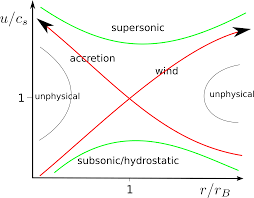
\includegraphics[width=0.75\linewidth]{Pictures/figures/bondi_regime.png}
    \caption{The parameter space of Bondi-accretion solutions. The sonic point $r_b$ is shown on the $x$-axis and the velocity on the $y$ axis.}
    \label{fig:bondi_regime}
\end{figure}
It is not immediately clear why we should have gone to all the work of building out this complicated ODE for ourselves; however, we can see that there are several very interesting features. The most important of these is that equation~\eqref{eq:bondi_critical_radius} is \textbf{singular} at 
\begin{equation}
    \label{eq:bondi_critical_radius}
    \boxed{
    r_s = \frac{GM}{2c_s^2}.
    }
\end{equation}
\rmk{Remember that $c_s$ is still a function of the radius. This means that this is \textbf{implicit}.} This is the so-called \textbf{sonic point} of the flow: \textit{if} the flow is going to make a transition to or from \textbf{sub-sonic} to \textbf{super-sonic}, it \textit{must occur at $r_s$.} This means that there are 4 important regimes to consider:
\vspace{0.5cm}
\begin{enumerate}
    \item \textbf{Transitioning Solution}: If we enforce that $u = c_s$ at the sonic radius, then the solution is entirely determined by the choice of behavior as $r\to \infty$ or by the choice of behavior as $r\to0$. If we let $u \to 0$ at $\infty$, then we obtain \textbf{accreting flows} featuring a transition point, and if we permit $u \to 0$ as $r\to 0$, then we obtain \textbf{wind flows} with transition points.
    \item \textbf{Non-Transitioning Solutions}: If a solution is not going to have $u=c_s$, then one \textit{must let $du^2/dr = 0$} at the sonic radius. In this case, the entire solution is fixed either by the behavior at either asymptote or by the behavior (the velocity) at the sonic point.
\end{enumerate}
\vspace{0.5cm}

\subsubsection{Bernoulli Flow}
We have now clarified the general behavior of the ODE we wish to solve and identified the relevant regimes. Most importantly, we are now able to recognize that uniqueness of our solution can be guaranteed by specifying the behavior both at the critical point and at $\infty$. Let us now fully solve the problem. To do so, we will apply \textbf{Bernoulli's Theorem}:
\[
u \frac{du}{dr}+ \nabla(h+\phi) = 0 \implies \frac{1}{2} u^2 + h + \phi = 0.
\]
For a \textbf{barotropic equation of state}, the specific enthalpy is
\[
h = \int \frac{dP}{\rho} = \int \frac{dP}{d\rho} \frac{1}{\rho} d\rho = \frac{K\gamma}{\gamma -1} \rho^{\gamma - 1} = \frac{c_s^2}{\gamma -1}.
\]
Thus,
\begin{equation}
    \frac{u^2}{2} + \frac{c_s^2}{\gamma -1} - \frac{GM}{r} = \rm{Constant}.
\end{equation}
\rmk{In the isothermal case, we actually need to have a logarithm here instead of $\gamma -1$.}
\par
Now, for \textbf{accreting flows}, we have $u(\infty) = 0$. Thus,
\[
c_s^2(\infty) = C(\gamma-1) \implies C = \frac{c_s^2(\infty)}{\gamma -1}.
\]
Additionally, the sonic point requires that
\[
c_s^2(r_s) = \frac{GM}{2r_s},
\]
so at $r_s$, we have
\[
\frac{c_s^2(r_s)}{2} + \frac{c_s^2(r_s)}{\gamma -1} - 2c_s^2(r_s) = \frac{c_s^2(\infty)}{\gamma -1}.
\]
So
\begin{equation}
\boxed{\
    c_s(r_s) = c_s(\infty) \left(\frac{2}{5 - 3\gamma}\right)^{1/2}
    }
\end{equation}
\rmk{Once again, we see that $\gamma = 5/3$ is not permitted! In practical scenarios, we are never really ideal, so this is fine, but nonetheless, it is worth noting.}
The mass accretion rate is constant at all radii, so we can evaluate it at the sonic point and find
\begin{equation}
    \boxed{
    \dot{M} = \pi G^2 M^2 \frac{\rho(\infty)}{c_s^3(\infty)} \left[\frac{2}{5-3\gamma}\right]^{(5-3\gamma)/2(\gamma-1)}.
    }
\end{equation}
\subsubsection{The Accretion Radius}

The Bondi solution motivates the introduction of a characteristic length scale, the
\textbf{accretion radius}, defined as
\begin{equation}
    \label{eq:bondi_radius}
    r_{\rm acc} \equiv \frac{2GM}{c_s^2(\infty)}.
\end{equation}
This can be understood from a simple energetic argument. At radius $r$, the
\textbf{gravitational binding energy per unit mass} is
\[
E_{\rm grav} \sim \frac{GM}{r},
\]
while the \textbf{thermal energy per unit mass} of the gas is set by the sound speed,
\[
E_{\rm th} \sim c_s^2(\infty).
\]
The radius $r_{\rm acc}$ is defined as the point where these two energy scales balance:
inside this radius, gravitational attraction dominates over thermal motions, so gas is
gravitationally captured by the accretor. Outside this radius, pressure forces can
support the gas against collapse. Thus, $r_{\rm acc}$ plays the role of an effective
``sphere of influence'' for accretion.

\begin{remark}
Note that $r_{\rm acc}$ is distinct from the precise sonic radius $r_s$, which depends
on the local sound speed $c_s(r_s)$. The accretion radius is defined in terms of the
\emph{asymptotic} sound speed at infinity, and provides a more intuitive, order-of-magnitude
measure of the capture region.
\end{remark}

\subsubsection{Free-Fall Behavior Beyond the Sonic Point}

Once the gas passes through the sonic point, the flow is \textbf{supersonic}. In this
regime, pressure forces are negligible compared to inertia and gravity: the gas
effectively undergoes free fall. This allows us to extract the asymptotic scaling of
velocity, density, and temperature in the inner region.

\paragraph{Velocity:} In free fall onto a point mass, the velocity is set by the
gravitational potential:
\[
u(r) \sim \left(\frac{2GM}{r}\right)^{1/2}.
\]

\paragraph{Density:} The accretion rate is constant at all radii,
\[
\dot{M} = 4\pi r^2 \rho u.
\]
Substituting the free-fall velocity,
\[
\rho(r) \sim \frac{\dot{M}}{4\pi r^2 u(r)} \;\propto\; r^{-3/2}.
\]

\paragraph{Temperature:} For a polytropic gas,
\[
T \propto \frac{P}{\rho} \propto \rho^{\gamma-1}.
\]
Thus, in the inner free-fall region,
\[
T(r) \;\propto\; r^{-3(\gamma-1)/2}.
\]
For example:
\begin{itemize}
    \item Isothermal case ($\gamma=1$): $T(r) = \rm{const}$.  
    \item Adiabatic monoatomic gas ($\gamma=5/3$): $T(r) \propto r^{-1}$.
\end{itemize}


\subsection*{Summary and Key Formulae}

Bondi accretion provides the simplest classical model for spherically symmetric accretion onto a compact object. While highly idealized, it illustrates several key physical principles:

\begin{itemize}
    \item The flow is uniquely determined by the requirement that it pass smoothly through the \textbf{sonic point}. This makes the solution transonic, subsonic at infinity and supersonic near the accretor. 
    \item The \textbf{accretion radius} 
    \[
    r_{\rm acc} = \frac{2GM}{c_s^2(\infty)}
    \]
    defines the natural scale inside which gravity dominates over thermal pressure. Gas at $r \lesssim r_{\rm acc}$ is gravitationally captured.
    \item The \textbf{Bondi accretion rate} can be expressed either in terms of $r_{\rm acc}$ or directly in terms of asymptotic conditions:
    \[
    \dot{M}_{\rm Bondi} \;\sim\; \pi r_{\rm acc}^2 \rho_\infty c_s(\infty),
    \qquad
    \dot{M}_{\rm Bondi} = \pi G^2 M^2 \frac{\rho(\infty)}{c_s(\infty)^3}\left[\frac{2}{5-3\gamma}\right]^{(5-3\gamma)/2(\gamma-1)}.
    \]
    The exact prefactor depends on the adiabatic index $\gamma$, but the scaling is robust.
    \item Inside the sonic point, the flow is effectively in free fall, with the following power-law scalings:
    \[
    u(r) \propto r^{-1/2}, \qquad \rho(r) \propto r^{-3/2}, \qquad T(r) \propto r^{-3(\gamma-1)/2}.
    \]
    For an adiabatic monoatomic gas ($\gamma=5/3$), this gives $T(r) \propto r^{-1}$.
    \item Order-of-magnitude estimates show that for compact objects, the rates are very small compared to what is observable:
    \[
    \dot{M}_{\rm Bondi} \sim 1.4 \times 10^{11}\;\; \left(\frac{M}{M_\odot}\right)^2 \left(\frac{\rho_\infty}{1\,{\rm cm}^{-3}\;m_p}\right)\left(\frac{10\,{\rm km/s}}{c_s(\infty)}\right)^3 \;{\rm g\,s^{-1}}.
    \]
    For example:
    \begin{itemize}
        \item White Dwarf ($M \sim 1M_\odot$, $R \sim 10^9\,$cm): $\dot{M} \sim 10^{12}\,{\rm g\,s^{-1}}$.
        \item Neutron Star ($M \sim 1.4M_\odot$, $R \sim 10^6\,$cm): $\dot{M} \sim 10^{13}\,{\rm g\,s^{-1}}$.
    \end{itemize}
    
Even though compact objects have deep gravitational potentials, the sparse interstellar medium is simply too dilute: Bondi accretion in realistic astrophysical settings is far below detectable levels.
\end{itemize}
\vspace{0.5cm}

\begin{bigidea}
\textbf{Bondi Accretion: Must-Remember Formulae}
\begin{align*}
r_{\rm acc} &= \frac{2GM}{c_s^2(\infty)} \\[6pt]
\dot{M}_{\rm Bondi} &\sim \pi r_{\rm acc}^2 \rho_\infty c_s(\infty) \;\;\;\; \propto \frac{(GM)^2 \rho_\infty}{c_s^3(\infty)} \\[6pt]
\rho(r) &\propto r^{-3/2}, \qquad T(r) \propto r^{-3(\gamma-1)/2}, \qquad u(r) \propto r^{-1/2} \\[6pt]
\dot{M}_{\rm WD} &\sim 10^{12} \;\left(\frac{M}{M_\odot}\right)^2\;{\rm g\,s^{-1}}, \qquad
\dot{M}_{\rm NS} \sim 10^{13} \;\left(\frac{M}{M_\odot}\right)^2\;{\rm g\,s^{-1}}
\end{align*}
\textbf{Takeaway:} Bondi accretion sets the baseline scale for spherical capture from a uniform medium, but the resulting accretion rates are far too small to be astrophysically significant in most environments.
\end{bigidea}
\end{document}
